%%
%% getstart.tex -- Flight Gear documentation: Installation and Getting Started
%% Master file
%%
%% Written by Michael Basler % Bernhard Buckel, starting September 1998.
%%
%% Copyright (C) 2002 Michael Basler  (pmb@epost.de)
%%                  & Bernhard Buckel (buckel@wmad95.mathematik.uni-wuerzburg.de)
%%
%% This program is free software; you can redistribute it and/or
%% modify it under the terms of the GNU General Public License as
%% published by the Free Software Foundation; either version 2 of the
%% License, or (at your option) any later version.
%%
%% This program is distributed in the hope that it will be useful, but
%% WITHOUT ANY WARRANTY; without even the implied warranty of
%% MERCHANTABILITY or FITNESS FOR A PARTICULAR PURPOSE.  See the GNU
%% General Public License for more details.
%%
%% You should have received a copy of the GNU General Public License
%% along with this program; if not, write to the Free Software
%% Foundation, Inc., 675 Mass Ave, Cambridge, MA 02139, USA.
%%
%% $Id: getstart.tex,v 0.6 2002/09/09 michael
%% (Log is kept at end of this file)

\documentclass[11pt,a4paper]{book}
\pagestyle{headings}
\usepackage[latin1]{inputenc}
\usepackage[T1]{fontenc}
\usepackage[pdftex]{graphics}
\usepackage{graphicx}
\usepackage[pdftex]{thumbpdf}
\usepackage{times}

\newcommand{\Index}[1]{#1\index{#1}}
\newcommand{\FlightGear}{{\itshape\bfseries FlightGear}}
\newcommand{\TerraGear}{{\itshape\bfseries TerraGear}}
\newcommand{\SimGear}{{\itshape\bfseries SimGear}}
\newcommand{\PLIB}{{\itshape\bfseries PLIB}}
\newcommand{\JSBSim}{{\itshape\bfseries JSBSim}}
\newcommand{\YASim}{{\itshape\bfseries YASim}}
\newcommand{\web}[1]{\href{#1}{#1}}
\newcommand{\mail}[1]{\href{mailto:#1}{#1}}
\newcommand{\Cygwin}{{\itshape\bfseries Cygwin}}

\newcommand{\longpage}{\enlargethispage{\baselineskip}}
\newcommand{\shortpage}{\enlargethispage{-\baselineskip}}

\makeindex
\usepackage{makeidx}
\makeglossary

\usepackage[
	pdftex,
	a4paper,
	bookmarks,
	bookmarksopen=true,
	bookmarksnumbered=true,
	pdfauthor={Hein Blvd},
	pdftitle={Meine Lebensgeschichte},
	colorlinks,
	linkcolor=blue,
	urlcolor=blue
]{hyperref}

\begin{document}
%%
%% getstart.tex -- Flight Gear documentation: The FlightGear Manual
%% Title file
%%
%% Written by Michael Basler, started September 1998.
%%
%% Copyright (C) 2002 Michael Basler
%%
%%
%% This program is free software; you can redistribute it and/or
%% modify it under the terms of the GNU General Public License as
%% published by the Free Software Foundation; either version 2 of the
%% License, or (at your option) any later version.
%%
%% This program is distributed in the hope that it will be useful, but
%% WITHOUT ANY WARRANTY; without even the implied warranty of
%% MERCHANTABILITY or FITNESS FOR A PARTICULAR PURPOSE.  See the GNU
%% General Public License for more details.
%%
%% You should have received a copy of the GNU General Public License
%% along with this program; if not, write to the Free Software
%% Foundation, Inc., 675 Mass Ave, Cambridge, MA 02139, USA.
%%
%% $Id: title.tex,v 0.6 2002/09/09 michael
%% (Log is kept at end of this file)

%%%%%%%%%%%%%%%%%%%%%%%%%%%%%%%%%%%%%%%%%%%%%%%%%%%%%%%%%%%%%%%%%%%%%%%%%%%%%%%%%%%%%%%%%%%%%%%
\title{The FlightGear Manual}
%%%%%%%%%%%%%%%%%%%%%%%%%%%%%%%%%%%%%%%%%%%%%%%%%%%%%%%%%%%%%%%%%%%%%%%%%%%%%%%%%%%%%%%%%%%%%%%

\author{
  Michael Basler, Martin Spott,\\
  Stuart Buchanan, Jon Berndt,\\
  Bernhard Buckel, Cameron Moore,\\
  Curt Olson, Dave Perry,\\
  Michael Selig, Darrell Walisser,\\
  and others\\
{ \setlength{\fboxsep}{12mm}\setlength{\fboxrule}{0pt}
 \centerline{\fbox{
\includegraphics[clip,width=10.0cm]{start2}
 }}}}

\date{The FlightGear Manual version 1.0\\
\today\\
For \FlightGear{} version 1.0}


\maketitle


\tableofcontents

%% Revision 0.00  1998/09/08  michael
%% Initial revision for version 0.53.
%% revision 0.10  1998/10/01  michael
%% final proofreading for release
%% revision 0.11  1998/11/01  michael
%% added title pic
%% revision 0.3 2000/04/20 michael
%% Remark for tracing version
%% revision 0.5.2 2002/XX/XX michael
%% glad to add several new contributors
%% revision 0.6 2002/09/05 michael
%% changed title picture
%% revision 0.7 2005/10/29 Stuart Buchanan
%% add self to contributors and updated datestamp

%%
%% getstart.tex -- Flight Gear documentation: The FlightGear Manual
%% Chapter file
%%
%% Written by Michael Basler, started September 1998.
%%
%% Copyright (C) 2002 Michael Basler
%%
%%
%% This program is free software; you can redistribute it and/or
%% modify it under the terms of the GNU General Public License as
%% published by the Free Software Foundation; either version 2 of the
%% License, or (at your option) any later version.
%%
%% This program is distributed in the hope that it will be useful, but
%% WITHOUT ANY WARRANTY; without even the implied warranty of
%% MERCHANTABILITY or FITNESS FOR A PARTICULAR PURPOSE.  See the GNU
%% General Public License for more details.
%%
%% You should have received a copy of the GNU General Public License
%% along with this program; if not, write to the Free Software
%% Foundation, Inc., 675 Mass Ave, Cambridge, MA 02139, USA.
%%
%% $Id: preface.tex,v 0.6 2002/09/09 michael
%% (Log is kept at end of this file)

%%%%%%%%%%%%%%%%%%%%%%%%%%%%%%%%%%%%%%%%%%%%%%%%%%%%%%%%%%%%%%%%%%%%%%%%%%%%%%%%%%%%%%%%%%%%%%%
\chapter*{Preface\label{preface}}
%%%%%%%%%%%%%%%%%%%%%%%%%%%%%%%%%%%%%%%%%%%%%%%%%%%%%%%%%%%%%%%%%%%%%%%%%%%%%%%%%%%%%%%%%%%%%%%

\FlightGear{} is a free Flight Simulator developed cooperatively over the Internet 
by a group of flight simulation and programming enthusiasts. "The
FlightGear Manual" is meant to give beginners a guide in getting
\FlightGear{} up and running, and themselves into the air. It is not
intended to provide complete documentation of all the features and
add-ons of \FlightGear{} but, instead, aims to give a new user the best
start to exploring what \FlightGear{} has to offer.

This version of the document was written for \FlightGear{} version 0.9.11. 
Users of earlier versions of \FlightGear{} will still find this document
useful, but some of the features described may not be present.

This guide is split into three parts and is structured as follows.

\medskip

\noindent
\textbf{Part I: Installation}
\medskip

 \noindent
Chapter~\ref{free}, \textit{Want to have a free flight? Take \FlightGear{}}, introduces
\FlightGear{}, provides background on the philosophy behind it and describes the system requirements.
 \medskip

 \noindent
In Chapter~\ref{prefligh}, \textit{Preflight: Installing \FlightGear{}}, you will find
instructions for installing the binaries\index{binary distribution} and additional scenery and aircraft. 
 \medskip

\noindent
\textbf{Part II: Flying with \FlightGear{}}
\medskip

 \noindent
  The following Chapter~\ref{takeoff}, \textit{Takeoff: How to start
  the program}, describes how to actually start the installed program.
  It includes an overview on the numerous command line options as well
  as configuration files.
 \medskip

 \noindent
  Chapter~\ref{flight}, \textit{In-flight: All about instruments,
  keystrokes and menus}, describes how to operate the program, i.\,e\.
  how to actually fly with \FlightGear{}\hspace{-1mm}. This includes a
  (hopefully) complete list of pre-defined keyboard commands, an
  overview on the menu entries, detailed descriptions on the instrument
  panel and HUD (head up display), as well as hints on using the mouse
  functions.
 \medskip

 \noindent
  Chapter~\ref{features}, \textit{Features}: Illustration of special
  features that \FlightGear{} offers to the advanced user.
 \medskip

\noindent
\textbf{Part III: Tutorials}
\medskip

 \noindent
 Chapter~\ref{tutorials}, \textit{Tutorials},
provides information on the many tutorials available for new pilots.
 \medskip

 \noindent
 Chapter~\ref{basic}, \textit{A Basic Flight Simulator Tutorial},
provides a tutorial on the basics of flying, illustrated with many
examples on how things actually look in \FlightGear{}.
 \medskip

 \noindent
 Chapter~\ref{crosscountry}, \textit{A Cross Country Flight Tutorial},
describes a simple cross-country flight in the San Fransisco area that
can be run with the default installation.
 \medskip

\noindent
\textbf{Appendices}
\medskip

 \noindent
  In Appendix~\ref{missed}, \textit{Missed approach: If anything refuses to work},
   we try to help you work through some common problems faced when using \FlightGear{}.
 \bigskip

 \noindent
Appendix~\ref{opengl}, \textit{OpenGL graphics drivers}, describes some
special problems you may encounter in case your system lacks support
for the OpenGL graphics API \Index{OpenGL} which \FlightGear{} is based
on.
 \medskip

 \noindent
 Appendix~\ref{building}, \textit{Building the plane: Compiling the program},
explains how to build (compile and link) the simulator. Depending on your platform this
may or may not be required. 
 \medskip

 \noindent
  In the final Appendix~\ref{landing}, \textit{Landing: Some further thoughts before leaving the plane}, we would like to give credit to those who deserve it, sketch an overview
on the development of \FlightGear and point out what remains to be done.
 \medskip

 \noindent
 Accordingly, we suggest reading the Chapters as follows:
 \medskip


\noindent
\begin{tabular}{ll}
 \textbf{Installation}                                  	&\\
 Users of binary distributions (notably under Windows):	 	&~\ref{prefligh}\\
 Installation under Linux/UNIX:               			&~\ref{building},~\ref{prefligh}\\
 Installation under Macintosh:               			&~\ref{prefligh}\\
  \textbf{Operation}                           			& \\
 Program start (all users):                      		&~\ref{takeoff}\\
 Keycodes, Panel, Mouse\ldots (all users):       		&~\ref{flight}\\
 \textbf{Troubleshooting}                      				& \\
 General issues:																						&~\ref{missed}\\
 Graphics problems: 									            				&~\ref{opengl}\\
 \textbf{Optionally}                           						&~\ref{free},~\ref{landing} 
\end{tabular}
\bigskip

\noindent
 While this introductory guide is meant to be self contained, we strongly suggest having a look into further documentation, especially in case of trouble:

\begin{itemize}
 \item For additional hints on troubleshooting and more, \textbf{please read the FAQ}\index{FAQ} 
 \medskip

 \noindent
 \web{http://www.flightgear.org/Docs/FlightGear-FAQ.html},
 
 The FAQ contains a host of valuable information, especially on rapidly changing flaws and additional reading, thus we strongly suggest consulting it in conjunction with our guide.
 
 
 \item A handy \textbf{leaflet}\index{leaflet} on operation for printout is available at
 \medskip

 \noindent
 \web{http://www.flightgear.org/Docs/InstallGuide/FGShortRef.html},
 \item Additional user documentation on special aspects is available within the base package under the directory \texttt{/FlightGear/Docs}.
 \end{itemize}

\noindent 
Finally:
\medskip


We know most people hate reading manuals. If you are sure the graphics driver for your card supports \Index{OpenGL} (check documentation; for instance all \Index{NVIDIA} Windows and Linux drivers for \Index{TNT}/TNT2/\Index{Geforce}/Geforce2/Geforce3 do) and if you are using one of the following operating systems:

\begin{itemize}
\item \Index{Windows} 95/98/ME/NT/2000/XP,
\item \Index{Macintosh} Mac OSX
\item \Index{Linux}
\item \Index{SGI Irix}
\end{itemize}

 \noindent
you can possibly skip at least Part I of this manual and exploit the pre-compiled binaries\index{binaries!pre-compiled}. These as well as instructions on how to set them up, can be found at
 \medskip

\web{http://www.flightgear.org/Downloads/}.
 \medskip

 \noindent
In case you are running \FlightGear{} on Linux, you may also be able to get binaries bundled with your distribution. Several vendors already include \FlightGear{} binaries into their distributions.
 
Just download them, install them according to the description and run them via the installed FlightGear icon (on Windows), or texttt{fgfs} having set the environmental variables described in Chapter \ref{takeoff} (on Linux).

There is no guarantee for this approach to work, though. If it doesn't, don't give up! Have a closer look through this guide notably Section~\ref{prefligh} and be sure to check out the \Index{FAQ}.


%% Revision 0.00  1998/09/08  michael
%% Initial revision for version 0.41.
%% Revision 0.01  2002/01/01 michael
%% Included outline of the Guide, integrated former separate chapter ''Quickstart''
%% revision 0.5 2002/01/01 michael/martin
%% Hint on Linux distros
%% revision 0.6 2002/09/09 michael
%% minor corrections
%% revision 0.7 2005/11.10 stuart
%% Changes for moving compilation information to appendix

\part{Installation}
%%
%% getstart.tex -- Flight Gear documentation: Installation and Getting Started
%% Chapter file
%%
%% Written by Michael Basler, started September 1998.
%%
%% Copyright (C) 2002 Michael Basler
%%
%%
%% This program is free software; you can redistribute it and/or
%% modify it under the terms of the GNU General Public License as
%% published by the Free Software Foundation; either version 2 of the
%% License, or (at your option) any later version.
%%
%% This program is distributed in the hope that it will be useful, but
%% WITHOUT ANY WARRANTY; without even the implied warranty of
%% MERCHANTABILITY or FITNESS FOR A PARTICULAR PURPOSE.  See the GNU
%% General Public License for more details.
%%
%% You should have received a copy of the GNU General Public License
%% along with this program; if not, write to the Free Software
%% Foundation, Inc., 675 Mass Ave, Cambridge, MA 02139, USA.
%%
%% $Id: free.tex,v 0.6 2002/09/09 michael
%% (Log is kept at end of this file)

%%%%%%%%%%%%%%%%%%%%%%%%%%%%%%%%%%%%%%%%%%%%%%%%%%%%%%%%%%%%%%%%%%%%%%%%%%%%%%%%%%%%%%%%%%%%%%%
\chapter{Want to have a free flight? Take {\FlightGear{}}!\label{free}}
%%%%%%%%%%%%%%%%%%%%%%%%%%%%%%%%%%%%%%%%%%%%%%%%%%%%%%%%%%%%%%%%%%%%%%%%%%%%%%%%%%%%%%%%%%%%%%%

%%%%%%%%%%%%%%%%%%%%%%%%%%%%%%%%%%%%%%%%%%%%%%%%%%%%%%%%%%%%%%%%%%%%%%%%%%%%%%%%%%%%%%%%%%%%%%%
\section{Yet Another Flight Simulator?}
%%%%%%%%%%%%%%%%%%%%%%%%%%%%%%%%%%%%%%%%%%%%%%%%%%%%%%%%%%%%%%%%%%%%%%%%%%%%%%%%%%%%%%%%%%%%%%%
\markboth{\thechapter.\hspace*{1mm} WANT TO HAVE A FREE FLIGHT?}{\thesection\hspace*{1mm}
YET ANOTHER FLIGHT SIMULATOR?}

Did you ever want to fly a plane yourself, but lacked the money or ability to do so? Are
you a real pilot looking to improve your skills without having to take off? Do you want
to try some dangerous maneuvers without risking your life? Or do you just want to have
fun with a more serious game without any violence? If any of these questions apply
to you, PC flight simulators are just for you.

You may already have some experience using \Index{Microsoft}'s {\copyright} Flight Simulator
or any other of the commercially available PC flight simulators. As the
price tag of those is usually within the {\$}50 range, buying one of them should not be a
serious problem given that running any serious PC flight simulator requires PC hardware
within the {\$}1500 range, despite dropping prices.

With so many commercially available flight simulators, why would we spend
thousands of hours of programming and design work to build a free flight
simulator?  Well, there are many reasons, but here are the major ones:

\begin{itemize}
 \item All of the commercial simulators have a serious drawback: they are made
 by a small group of developers defining their properties according to what
 is important to them and providing limited interfaces to end users.  Anyone
 who has ever tried to contact a commercial developer would agree that getting
 your voice heard in that environment is a major challenge.  In contrast,
 \FlightGear{} is designed by the people and for the people with everything
 out in the open.

 \item Commercial simulators are usually a compromise of features and
 usability.  Most commercial developers want to be able to serve a broad
 segment of the population, including serious pilots, beginners, and even
 casual gamers.
 In reality the result is always a compromise due to deadlines and
 funding.  As \FlightGear{} is free and open, there is no need for such
 a compromise.  We have no publisher breathing down our necks, and
 we're all volunteers that make our own deadlines.  We are also at
 liberty to support markets that no commercial developer would consider
 viable, like the scientific research community.
 \item Due to their closed-source nature, commercial simulators keep developers
 with excellent ideas and skills from contributing to the products.  With
 \FlightGear{}, developers of all skill levels and ideas have the potential
 to make a huge impact on the project.  Contributing to a project as large
 and complex as \FlightGear{} is very rewarding and provides the developers
 with a great deal of pride in knowing that we are shaping the future of a
 great simulator.
 \item Beyond everything else, it's just plain fun!  I suppose you could
 compare us to real pilots that build kit-planes or scratch-builts.  Sure,
 we can go out a buy a pre-built aircraft, but there's just something special
 about building one yourself.
\end{itemize}

The points mentioned above form the basis of why we created \FlightGear{}.
With those motivations in mind, we have set out to create a high-quality
flight simulator that aims to be a civilian,\index{Flight simulator!civilian}
multi-platform,\index{Flight simulator!multi-platform} open,\index{Flight simulator!open}
user-supported,\index{Flight simulator!user-sported} and user-extensible\index{Flight
simulator!user-extensible} platform.  Let us take a closer look at each of these
characteristics:

\begin{itemize}
 \item \textbf{Civilian:}\index{Flight simulator!civilian} The project is primarily aimed
 at civilian flight simulation.  It should be appropriate for simulating general aviation
 as well as civilian aircraft.  Our long-term goal is to have \FlightGear{} FAA-approved as
 a flight training device.  To the disappointment of some users, it is currently not a
 combat simulator; however, these features are not explicitly excluded.  We just have
 not had a developer that was seriously interested in systems necessary for combat
 simulation.

 \item\textbf{Multi-platform:}\index{Flight simulator!multi-platform} The
 developers are attempting to keep the code as platform-independent as possible. This
 is based on their observation that people interested in flight simulations run quite a
 variety of computer hardware and operating systems. The present code supports the
 following \Index{Operating Systems}:
  \begin{itemize}
  \item\Index{Linux} (any distribution and platform),
  \item\Index{Windows NT/2000/XP} (Intel/AMD platform),
  \item\Index{Windows 95/98/ME},
  \item\Index{BSD UNIX},
  \item\Index{SGI IRIX},
  \item\Index{Sun-OS},
  \item{Macintosh.}
  \end{itemize}

At present, there is no known flight simulator -- commercial or free -- supporting such a
broad range of platforms.

  \item\textbf{Open:}\index{Flight simulator!open} The project is not restricted to a
  static or elite cadre of developers. Anyone who feels they are able to contribute
  is most welcome.  The code (including documentation) is copyrighted under the
  terms of the \Index{GNU General Public License} (\Index{GPL}).

  The \Index{GPL} is often misunderstood. In simple terms it
  states that you can copy and freely distribute the program(s) so licensed.
  You can modify them if you like and even charge as much money as want to for the
  distribution of the modified or original program.  However, you must freely provide
  the entire source code to anyone who wants it, and it must retain the original copyrights.
  In short:
\medskip

\centerline{\textit{''You can do anything with the software except make it non-free''}.}

The full text of the \Index{GPL} can be obtained from the \FlightGear{} source code or from
 \medskip

\web{http://www.gnu.org/copyleft/gpl.html}.
 \medskip

\item\textbf{User-supported and user-extensible:}\index{Flight simulator!user-supported}
  \index{Flight simulator!user-extensible} Unlike most commercial simulators,
  \FlightGear{}'s scenery and aircraft formats, internal variables, APIs, and everything
  else are user accessible and documented from the beginning. Even without any explicit
  development \Index{documentation} (which naturally has to be written at some point),
  one can always go to the \Index{source code} to see how something works. It is the
  goal of the developers to build a basic engine to which scenery designers, panel
  engineers, maybe adventure or ATC routine writers, sound artists, and others can build
  upon. It is our hope that the project, including the developers and end users, will
  benefit from the creativity and ideas of the hundreds of talented ``simmers'' around
  the world.
\end{itemize}

  Without doubt, the success of the \Index{Linux} project, initiated by Linus
  Torvalds,\index{Torvalds, Linus} inspired several of the developers.
  Not only has \Index{Linux} shown that distributed development of highly
  sophisticated software projects over the Internet is possible, it has also
  proven that such an effort can surpass the level of quality of competing
  commercial products.
\medskip

 \centerline{\fbox{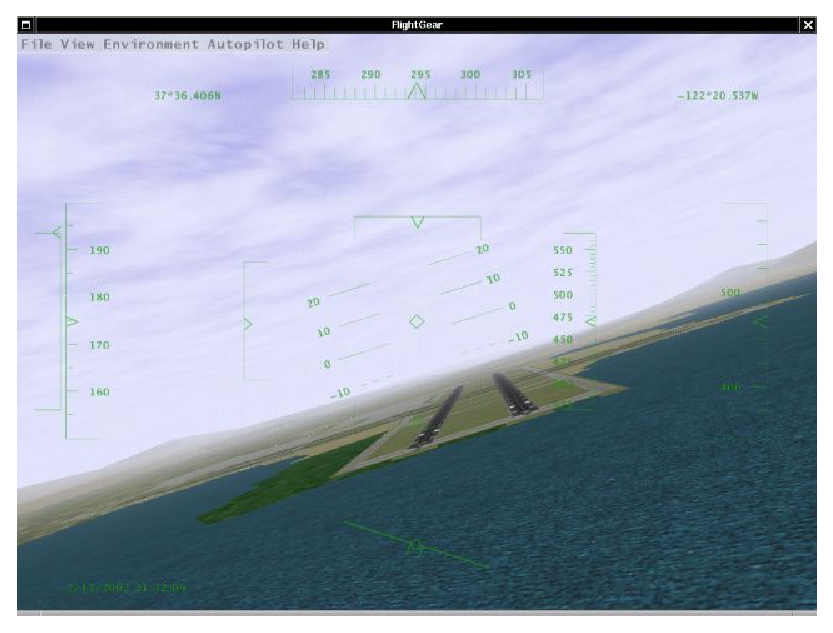
\includegraphics[clip,width=12.5cm]{KSFOapp}
}}

\smallskip
 \noindent
Fig.\,1: \textit{\FlightGear{} under UNIX: Bad approach to San Francisco International - by one of the authors of this manual\ldots}

%%%%%%%%%%%%%%%%%%%%%%%%%%%%%%%%%%%%%%%%%%%%%%%%%%%%%%%%%%%%%%%%%%%%%%%%%%%%%%%%%%%%%%%%%%%%%%%
\section{System Requirements}\index{system requirements}
%%%%%%%%%%%%%%%%%%%%%%%%%%%%%%%%%%%%%%%%%%%%%%%%%%%%%%%%%%%%%%%%%%%%%%%%%%%%%%%%%%%%%%%%%%%%%%%
In comparison to other recent flight simulators, the \Index{system requirements} for
\FlightGear{} are not extravagant. A decent PIII/800, or something in that range, should be
sufficient given you have a proper 3-D \Index{graphics card}. Additionally, any
modern \Index{UNIX}-type \Index{workstation} with a 3-D graphics card will handle
\FlightGear{} as well.

One important prerequisite for running \FlightGear{} is a graphics card whose driver supports
\Index{OpenGL}. If you don't know what \Index{OpenGL} is, the overview given at the OpenGL website
\medskip

\web{http://www.opengl.org}
\medskip

\noindent
 says it best: ``Since its introduction in 1992, OpenGL has become the
industry's most widely used and supported 2-D and 3-D graphics application programming
interface (API)...''.

\FlightGear{} does not run (and will never run) on a graphics board which only supports
\Index{Direct3D}. Contrary to OpenGL, Direct3D is a proprietary interface, being restricted to
the Windows operating system.

You may be able to run \FlightGear{} on a computer that features a 3-D video card not
supporting hardware accelerated \Index{OpenGL} -- and even on systems without 3-D
graphics hardware at all. However, the absence of hardware accelerated OpenGL support can bring even the fastest machine to its knees. The typical signal for missing hardware acceleration
are \Index{frame rate}s below 1 frame per second.

Any modern 3-D graphics featuring \Index{OpenGL} support will do. For
\Index{Windows} video card drivers that support OpenGL, visit the home page of your video
card manufacturer. You should note that sometimes OpenGL drivers\index{OpenGL!drivers}
are provided by the manufacturers of the graphics chip instead of by the makers of the
board. If you are going to buy a graphics card for running \FlightGear{}, one based on a
NVIDIA chip (TNT X/Geforce X) might be a good choice.

To install the executable and basic scenery, you will need around 50 MB of free \Index{disk
space}. In case you want/have to compile the program yourself you will need about an additional
500 MB for the source code and for temporary files created during compilation. This does not
include the development environment, which will vary in size depending on the operating system
and environment being used.  Windows users can expect to need approximately 300 MB of additional
disk space for the development environment.  Linux and other UNIX machines should have most of
the development tools already installed, so there is likely to be little additional space
needed on those platforms.

For the \Index{sound effects}, any capable \Index{sound card} should suffice.
Due to its flexible design, \FlightGear{} supports a wide range of \Index{joysticks} and
\Index{yokes} as well as \Index{rudder pedals} under \Index{Linux} and \Index{Windows}. 
\FlightGear{} can also provide interfaces to full-motion flight chairs.

\FlightGear{} is being developed primarily under \Index{Linux}, a free UNIX clone
(together with lots of GNU utilities) developed cooperatively over the Internet in much
the same spirit as \FlightGear{} itself. \FlightGear{} also runs and is partly developed
under several flavors of \Index{Windows}. Building \FlightGear{} is also possible on a Macintosh OSX
and several different UNIX/X11 workstations. Given you have a proper \Index{compiler} installed,
\FlightGear{} can be built under all of these platforms. The primary compiler for all platforms is
the free \Index{GNU C++} compiler (the \Index{Cygnus} \Index{Cygwin} compiler under Win32).

If you want to run \FlightGear{} under Mac OSX we suggest a Power PC G3 300 MHz or better. As a
graphics card we would suggest an ATI Rage 128 based card as a minimum. Joysticks are supported
under Mac OS 9.x only; there is no joystick support under Max OSX at this time.


%%%%%%%%%%%%%%%%%%%%%%%%%%%%%%%%%%%%%%%%%%%%%%%%%%%%%%%%%%%%%%%%%%%%%%%%%%%%%%%%%%%%%%%%%%%%%%%
\section{Choosing A Version}\index{FlightGear!versions}
%%%%%%%%%%%%%%%%%%%%%%%%%%%%%%%%%%%%%%%%%%%%%%%%%%%%%%%%%%%%%%%%%%%%%%%%%%%%%%%%%%%%%%%%%%%%%%%

Concerning the \FlightGear{} source code there exist two branches, a stable branch and a
developmental branch.\index{branch, stable}\index{branch, developmental} Even version numbers
like 0.6, 0.8, and (someday hopefully) 1.0 refer to stable releases, while odd
numbers like 0.7, 0.9, and so on refer to developmental releases. The policy is to only do
bug fixes in the even versions, while new features are generally added to odd-numbered
versions which, after all things have stabilized, will become the next stable release
with a version number calculated by adding 0.1.\label{branches}

To add to the confusion, there usually are several versions of the ``unstable''
branch. First, there is a ``latest official release'' which the pre-compiled binaries are based
on.  It is available from
\medskip

\web{ftp://ftp.flightgear.org/pub/fgfs/Source/FlightGear-X.Y.Z.tar.gz}
\medskip

For developers there exist CVS snapshots\index{CVS snapshots}\index{nightly snapshots} of the
source code, available from
 \medskip

\web{ftp://www.flightgear.org/pub/flightgear/Devel/Snapshots/}.
 \medskip

 \noindent
While theses are quite recent, they may still be sometimes a few days back behind
development. Thus, if you really want to get the very latest and greatest (and, at times,
buggiest) code, you can use a tool called \Index{anonymous cvs}\index{cvs, anonymous}
available from
 \medskip

\web{http://www.cvshome.org/}
 \medskip

 \noindent
to get the recent code. A detailed description of how to set this up for \FlightGear{}
can be found at
 \medskip

\web{http://www.flightgear.org/cvsResources/}.
 \medskip

 \noindent
 Unfortunately, the system implemented above does not really work as it should. As a matter of
 fact, the stable version is usually so much outdated, that it does not at all reflect the state
 of development \FlightGear{} has reached. Given that the recent developmental versions on the
 other hands may contain bugs (\ldots undocumented features), we recommend using the
 ``latest official (unstable) release'' for the average user. This is the latest version named at

 \web{http://www.flightgear.org/News/};
 \medskip

\noindent
 usually this is also the version which the binary distributions\index{distribution!binary}
 available at
 \medskip

\web{http://www.flightgear.org/Downloads/}
 \medskip

 \noindent
 are based on. If not otherwise stated, all procedures in this ``Installation and Getting Started''
 will be based on these packages.

%%%%%%%%%%%%%%%%%%%%%%%%%%%%%%%%%%%%%%%%%%%%%%%%%%%%%%%%%%%%%%%%%%%%%%%%%%%%%%%%%%%%%%%%%%%%%%%
\section{Flight Dynamics Models\label{flightmodels}}\index{flight dynamics model}\index{flight model}
%%%%%%%%%%%%%%%%%%%%%%%%%%%%%%%%%%%%%%%%%%%%%%%%%%%%%%%%%%%%%%%%%%%%%%%%%%%%%%%%%%%%%%%%%%%%%%%
Historically, \FlightGear{} has been based on a flight model it inherited (together
with the Navion airplane) from LaRCsim. As this had several limitations (most important,
many characteristics were hard wired in contrast to using configuration files), there were
several attempts to develop or include alternative \Index{flightmodels}. As a result,
\FlightGear{} supports several different flight models, to be chosen from at runtime.

The most important one is the JSB flight model developed by Jon Berndt. Actually, the JSB
flight model is part of a stand-alone project called \JSBSim, having its home at
 \medskip

\web{http://jsbsim.sourceforge.net/}.
 \medskip

 \noindent
Concerning airplanes, the JSB flight model at present provides support for a
\Index{Cessna 172}, a \Index{Cessna 182}, a \Index{Cessna 310}, and for an experimental plane
called \Index{X15}. Jon and his group are gearing towards a very accurate flight model, and the
JSB model has become \FlightGear{}'s default flight model.

As an interesting alternative, Christian Mayer developed a flight model of a hot air
balloon. Moreover, Curt Olson integrated a special ``UFO'' slew mode, which
helps you to quickly fly from point A to point B.

Recently, Andrew Ross contributed another flight model called \YASim{}\index{YASim} for
\textit{Yet Another Simulator}. At present, it sports another \Index{Cessna 172}, a
\Index{Turbo 310}, a fairly good \Index{DC-3} model, along with a \Index{Boeing 747},
\Index{Harrier}, and \Index{A4}. \YASim{} takes a fundamentally different approach since it's
based on geometry information rather than aerodynamic coefficients. Where \JSBSim{} will be exact for every situation that is known and flight tested, but may have odd and/or unrealistic behavior outside normal flight, \YASim{} will be sensible and consistent in almost every flight situation, but is likely to differ in performance numbers.

As a further alternative, there is the \Index{UIUC flight model}, developed by a 
team at the University of Illinois at Urbana-Champaign.  This work was 
initially geared toward modeling aircraft in icing conditions\index{icing!modelling} together with a smart icing system to better enable pilots to fly safely in an icing 
encounter.  While this research continues, the project has expanded to 
include modeling ``nonlinear'' aerodynamics, which result in more realism 
in extreme attitudes, such as stall and high angle of attack flight.  Two 
good examples that illustrate this capability are the \Index{Airwave Xtreme 150} 
\Index{hang glider} and the 1903 \Index{Wright Flyer}.  For the hang glider, throttle can 
be use to fly to gliding altitude or Ctrl-U can be used to jump up in 
1000-ft increments.  Try your hand at the unstable Wright Flyer and don't 
stall the canard!  Considerable up elevator trim will be required for level 
flight.  In general, the aerodynamics are probably very close to the 
original Wright Flyer as they are partly based on experimental data taken 
on a replica tested recently at the NASA Ames Research Center.  Also 
included are two more models, a \Index{Beech 99} and \Index{Marchetti S-211} jet trainer, 
which are older generation UIUC/FGFS models and based on simpler ``linear'' 
aerodynamics.  More details of the UIUC flight model and a list of aircraft 
soon to be upgraded can be found on their website at
\medskip

\href{http://amber.aae.uiuc.edu/~m-selig/apasim.html}{http://amber.aae.uiuc.edu/\~{}m-selig/apasim.html}
\medskip

\noindent
Note that the 3D models of the UIUC airplanes\index{UIUC airplanes!3D models} can be downloaded from a site maintained by Wolfram Kuss
\medskip

\web{http://home.t-online.de/home/Wolfram.Kuss/}
\medskip

It is even possible to drive FlightGear's scene display using an external
FDM\index{FDM!external} running on a different computer or via named
pipe\index{FDM!pipe} on the local machine -- although this might not be a
setup recommended to people just getting in touch with \FlightGear.


%%%%%%%%%%%%%%%%%%%%%%%%%%%%%%%%%%%%%%%%%%%%%%%%%%%%%%%%%%%%%%%%%%%%%%%%%%%%%%%%%%%%%%%%%%%%%%%
\section{About This Guide}
%%%%%%%%%%%%%%%%%%%%%%%%%%%%%%%%%%%%%%%%%%%%%%%%%%%%%%%%%%%%%%%%%%%%%%%%%%%%%%%%%%%%%%%%%%%%%%%
\markright{\thesection.\hspace*{1mm} ABOUT THIS GUIDE}

There is little, if any, material in this Guide that is presented here exclusively. You
could even say with Montaigne that we ``merely gathered here a big bunch of other men's
flowers, having furnished nothing of my own but the strip to hold them together''. Most
(but fortunately not all) of the information herein can also be obtained from the
\FlightGear{} web site\index{FlightGear Website} located at
\medskip

\web{http://www.flightgear.org/}
\medskip

Please, keep in mind that there are several mirrors of the \FlightGear{} web sites, all
of which are linked to from the \FlightGear{} homepage listed above.
You may prefer to download \FlightGear{} from a mirror closer to you than from the
main site.

This \textit{\FlightGear{} Installation and Getting Started} manual is intended to be a
first step towards a complete \FlightGear{} documentation\index{FlightGear
documentation}. The target
audience is the end-user who is not interested in the internal workings of \Index{OpenGL}
or in building his or her own scenery. It is our hope, that someday there
will be an accompanying \textit{\FlightGear{} Programmer's Guide}\index{FlightGear
Programmer's Guide} (which could be based on some of the documentation found at
 \medskip

\web{http://www.flightgear.org/Docs};
 \medskip

 \noindent
a \textit{\FlightGear{} Scenery Design Guide},\index{FlightGear Scenery Design Guide}
describing the Scenery tools now packaged as \TerraGear{}; and a \textit{\FlightGear{}
Flight School}\index{FlightGear Flight School} package.
 \medskip

As a supplement, we recommend reading the \FlightGear{} FAQ to be found at

\web{http://www.flightgear.org/Docs/FlightGear-FAQ.html}

which has a lot of supplementary information that may not be included in this manual.

\textbf{We kindly ask you to help us refine this document by submitting corrections,
improvements, and suggestions. All users are invited to contribute descriptions of alternative
setups (graphics cards, operating systems etc.). We will be more than happy to include
those into future versions of this \textit{Installation and Getting Started} (of course
not without giving credit to the authors).}

While we intend to continuously update this document, we may not be able to produce a
new version for every single release of {\FlightGear{}}.  To do so would require more
manpower that we have now, so please feel free to jump in and help out.  We hope to
produce documentation that measures up to the quality of \FlightGear{} itself.


%% Revision 0.00  1998/09/08  michael
%% Initial revision for version 0.53.
%% Revision 0.01  1998/09/20  michael
%% several extensions and corrections
%% revision 0.10  1998/10/01  michael
%% final proofreading for release
%% revision 0.11  1998/11/01  michael
%% minor corrections on platforms, satellite data, OpenGL
%% added Navion pic
%% revision 0.12  1999/03/07  michael
%% update on recent development
%% revision 0.20  1999/06/04  michael
%% updates on recent development, corrections of links
%% revision 0.3 2000/04/20 michael
%% Rewritten for version 0.7.2, many changes, added development since summer 1999,
%% development vs. stable version, split into SimGear/FlightGear/TerraGear
%% Proofread by Jon Berndt
%% revision 0.4 2001/05/12 michael
%% update on development during the last year, corrections on requirements,
%% new sections on different versions and on flight models
%% revision 0.41 2001/07/01 martin & michael
%% comment on external FDM
%% hint to FAQ
%% extended remarks on property manager
%% revision 0.5 2002/01/01 michael
%% several minor updates, corrected links
%% Hint on YASim by Martin
%% Picture KSFOapp added by Martin
%% System requirements contributed from Darrell
%% revision 0.6 2002/02/23 cameron
%% Many, many corrections
%% Rewrote several parts
%% Changed section titles
%% revision 0.6 2002/09/07 michael
%% Added contribution by M Selig on UIUC models
%% 3 minor typo/grammar edits by Dave Perry 
%% (P.12 replaced double apostrophe, p.14 <<<to to  >>> to, <<<users is >>>users are

%%
%% getstart.tex -- Flight Gear documentation: The FlightGear Manual
%% Chapter file
%%
%% Written by Michael Basler % Bernhard Buckel, starting September 1998.
%%
%% Copyright (C) 2002 Michael Basler
%%                  & Bernhard Buckel
%%
%% This program is free software; you can redistribute it and/or
%% modify it under the terms of the GNU General Public License as
%% published by the Free Software Foundation; either version 2 of the
%% License, or (at your option) any later version.
%%
%% This program is distributed in the hope that it will be useful, but
%% WITHOUT ANY WARRANTY; without even the implied warranty of
%% MERCHANTABILITY or FITNESS FOR A PARTICULAR PURPOSE.  See the GNU
%% General Public License for more details.
%%
%% You should have received a copy of the GNU General Public License
%% along with this program; if not, write to the Free Software
%% Foundation, Inc., 675 Mass Ave, Cambridge, MA 02139, USA.
%%
%% $Id: building.tex,v 0.6 2002/09/09 michael
%% (Log is kept at end of this file)

%%%%%%%%%%%%%%%%%%%%%%%%%%%%%%%%%%%%%%%%%%%%%%%%%%%%%%%%%%%%%%%%%%%%%%%%%%%%%%%%%%%%%%%%%%%%%%
\chapter{Building the plane: Compiling\index{compiling} the program\label{building}}
%%%%%%%%%%%%%%%%%%%%%%%%%%%%%%%%%%%%%%%%%%%%%%%%%%%%%%%%%%%%%%%%%%%%%%%%%%%%%%%%%%%%%%%%%%%%%%
\markboth{\thechapter.\hspace*{1mm} BUILDING THE
PLANE}{\thesection\hspace*{1mm} COMPILING UNDER LINUX}

This appendix describes how to build \FlightGear{} on several systems. In case you
are on a Win32 (i.\,e. Windows95/98/ME/NT/2000/XP) platform or any of the other platforms
for which binary executables are available, you may not want to go through that
potentially troublesome process but skip this section for now and go back to the
chapter on installing \FlightGear{} one. (Not everyone wants to build his or her plane
himself or herself, right?)
However, there may be good reason for at least trying to build the simulator:

\begin{itemize}
\item In case you are on a \Index{UNIX}/\Index{Linux} platform there may be no
pre-compiled binaries\index{binaries, pre-compiled} available for your system. In
practice it is common to install programs like this one on \Index{UNIX} systems by
recompiling them.

\item There are several options you can set during compile time only.

\item You may be proud you did.
\end{itemize}

On the other hand, compiling \FlightGear{} is not a task for novice users. Thus, if
you're a beginner (we all were once) on a platform which \Index{binaries} are available
for, we recommend postponing this task and just starting with the binary
distribution\index{distribution!binary} to get you flying.

As you will notice, this Chapter is far from being complete. Basically, we describe
compiling for two operating systems only, \Index{Windows} and \Index{Linux}, and for only
one compiler, the GNU C compiler. \FlightGear{} has been shown to be built under
different compilers (including Microsoft Visual C) as well as different systems
(Macintosh) as well. The reason for these limitations are:

\begin{itemize}
\item Personally, we have access to a Windows machine running the Cygnus compiler only.
\item According to the mailing lists, these seem to be the systems with the largest user base.
\item These are the simplest systems to compile \FlightGear{} on. Other compilers may need special
add-ons (workplace etc.) or even modification of the code.
\item The GNU compiler is free in the same sense of the GPL as \FlightGear{} is.
\end{itemize}

You might want to check Section~\ref{missed}, \textit{Missed approach},
if anything fails during compilation. In case this does not help we
recommend sending a note to one of the mailing lists (for hints on
subscription see Chapter~\ref{landing}).

There are several \Index{Linux distributions} on the market, and most
of them should work. Some come even bundled with (often outdated)
versions of \FlightGear{}. However, if you are going to download or
buy a distribution, \Index{Debian} (Sarge) is highly recommended by most people.
\Index{SuSE} and Ubuntu works well, too.

Contrary to Linux/Unix systems, Windows usually comes without any development tools. This
way, you first have to install a development environment. On Windows, in a sense, before
building the plane you will have to build the plant for building planes. This will be the
topic of the following section, which can be omitted by Linux users.

%%%%%%%%%%%%%%%%%%%%%%%%%%%%%%%%%%%%%%%%%%%%%%%%%%%%%%%%%%%%%%%%%%%%%%%%%%%%%%%%%%%%%%%%%%%%%%
\section{Preparing the \Index{development environment} under Windows\label{preparewin}}
%%%%%%%%%%%%%%%%%%%%%%%%%%%%%%%%%%%%%%%%%%%%%%%%%%%%%%%%%%%%%%%%%%%%%%%%%%%%%%%%%%%%%%%%%%%%%%

There is a powerful development environment available for Windows and this even for free:
The Cygnus development tools,\index{Cygnus!development tools} resp. \Cygwin. Their home
is at
 \medskip

\web{http://sources.redhat.com/cygwin/},
 \medskip

 \noindent
and it is always a good idea to check back what is going on there now and then.

Nowadays, installing \Cygwin{}\index{Cygwin!setup} is nearly automatic.
First, make sure the drive you want \Cygwin{}, \OSG{}, \PLIB{},
\SimGear{} and \FlightGear{} to live on, has nearly 1 GB of free
\Index{disk space}. Create a temporary directory and download the
installer from the site named above to that directory. (While the
installer does an automatic installation of the Cygnus environment, it
is a good idea to download a new installer from time to time.)

Invoke the installer now. It gives you three options. To avoid having to download stuff
twice in case of a re-installation or installation on a second machine, we highly
recommended to take a two-step procedure. First, select the option \texttt{Download from
Internet}. Insert the path of your temporary directory, your Internet connection settings
and then choose a mirror form the list. Near servers might be preferred, but may be
sometimes a bit behind with mirroring. We found
\medskip

\web{ftp://mirrors.rcn.net}
\medskip

 \noindent
a very recent and fast choice. In the next windows the default settings are usually a
good start. Now choose \texttt{Next}, sit back and wait.

If you are done, invoke the installer another time, now with the option
\texttt{Install from local directory}. After confirming the temporary directory you can
select a root directory (acting as the root directory of your pseudo UNIX file system).
Cygnus does not recommend taking the actual root directory of a drive, thus choose
\texttt{c:/Cygwin}
(while other drives than \texttt{c:} work as well). Now, all \Cygwin{}
stuff and all \FlightGear{} stuff lives under this directory. In
addition, select

 \texttt{Default text file type: Unix}

\noindent
 In addition, you have the choice to install the compiler for all users or just for you.
 
  The final window before installation gives you a selection of
  packages to install. It is hard, to provide a minimum selection of
  packages required for \FlightGear{} and the accompanying libraries to
  install. We have observed the following (non minimum) combination to
  work:\index{Cygwin!packages to install}
  
  \begin{itemize}
  \item{\texttt{Admin}} skip
  \item{\texttt{Archive}} install
  \item{\texttt{Base}} install
  \item{\texttt{Database}} skip
  \item{\texttt{Devel}} install
  \item{\texttt{Doc}} install
  \item{\texttt{Editors}} skip
  \item{\texttt{Graphics}} install
  \item{\texttt{Interpreters}} install
  \item{\texttt{Libs}} install
  \item{\texttt{Mail}} skip
  \item{\texttt{Net}} skip
  \item{\texttt{Shells}} install
  \item{\texttt{Text}} install
  \item{\texttt{Utils}} install
  \item{\texttt{Web}} skip
  \item{\texttt{XFree86}} do not install!
  \end{itemize}

\textbf{Note} XFree86\index{Cygwin!XFree86} must be not installed for building \FlightGear{} and the accompanying libraries. If it is installed you have to deinstall it first. Otherwise \FlightGear{}'s configuration scripts will detect the XFree86 OpenGL libraries and link to them, while the code is not prepared to do so.

As a final step you should include the \Index{binary directory} (for instance:\\
\texttt{c:/Cygwin/bin}) into your path by adding \verb/path=c:\Cygwin\bin/ in
your \texttt{autoexec.bat} under Windows 95/98/ME\. Under
WindowsNT/2000/XP, use the \texttt{Extended} tab under the
\texttt{System properties} page in Windows \texttt{control panel}.
There you'll find a button \texttt{Environment variables}, where you
can add the named directory.

Now you are done. Fortunately, all this is required only once. At this point you have
a nearly UNIX-like (command line) development environment. Because of this, the following
steps are nearly identical under Windows and Linux/Unix.

%%%%%%%%%%%%%%%%%%%%%%%%%%%%%%%%%%%%%%%%%%%%%%%%%%%%%%%%%%%%%%%%%%%%%%%%%%%%%%%%%%%%%%%%%%%%%%
\section{Preparing the \Index{development environment} under Linux\label{preparelin}}
%%%%%%%%%%%%%%%%%%%%%%%%%%%%%%%%%%%%%%%%%%%%%%%%%%%%%%%%%%%%%%%%%%%%%%%%%%%%%%%%%%%%%%%%%%%%%%
Linux, like any UNIX, usually comes with a compiler pre-installed. On
the other hand, you still have to make sure several required libraries
are present.

First, make sure you have all necessary OpenGL libraries. Fortunately,
most of the recent Linux distributions (i.e. SuSE-7.3) put these
already into the right place. (There have been reports, though, that on
Slackware you may have to copy the libraries to \texttt{/usr/local/lib}
and the headers to \texttt{/usr/local/include} by hand after building
\texttt{glut-3.7}). Be sure to install the proper packages: Besides the
basic X11 stuff you want to have - SuSE as an example - the following
packages: mesa, mesa-devel, mesasoft, xf86\_glx, xf86glu,
xf86glu-devel, mesaglut, mesaglut-devel and plib.

Also you are expected to have a bunch of tools installed that are usually
required to compile the Linux kernel. So you may use the Linux kernel source
package to determine the required dependencies. The following packages
might prove to be useful when fiddling with the \FlightGear{} sources:
automake, autoconf, libtool, bison, flex and some more, that are not
required to build a Linux kernel.

{\bfseries Please compare the release of the plib library with the one that ships with
your Linux distribution.} It might be the case that \FlightGear{} requires a
newer one that is not yet provided by your vendor.

%%%%%%%%%%%%%%%%%%%%%%%%%%%%%%%%%%%%%%%%%%%%%%%%%%%%%%%%%%%%%%%%%%%%%%%%%%%%%%%%%%%%%%%%%%%%%%
\section{One-time preparations for Linux and Windows users\label{preparelinwin}}
%%%%%%%%%%%%%%%%%%%%%%%%%%%%%%%%%%%%%%%%%%%%%%%%%%%%%%%%%%%%%%%%%%%%%%%%%%%%%%%%%%%%%%%%%%%%%%

There are a couple of 3rd party libraries which your Linux or Windows
system may or may not have installed, i.e\. the \textbf{\textit{ZLIB}}
library. You can either check your list of installed packages or just
try building \SimGear{}: It should exit and spit an error message
(observe this!) if one of these libraries is missing.

If you make this observation, install the missing libraries, which is
only required once (unless you re-install your development
environment).

Both libraries come bundled with \SimGear{}, which links to them, but
does not automatically install them. For installing either of them, get
the most recent file \texttt{SimGear-X.X.X.tar.gz}\index{SimGear} from
  \medskip

\web{http://www.simgear.org/downloads.html}
   \medskip

 \noindent
Download it to \texttt{/usr/local/source}. Change to that directory and unpack \SimGear{}
using

        \texttt{tar xvfz SimGear-X.X.X.tar.gz}.

You will observe a directory \texttt{src-libs} which contains the two names libraries. 

\subsection{Installation of \textbf{\textit{ZLIB}\index{ZLIB!installation}\label{zlibinstall}}}

\noindent
 \texttt{cd} into \texttt{SimGear-X.X.X/scr-libs} and unpack \textbf{\textit{ZLIB}} using
 \medskip
 
 \noindent
 				\texttt{tar xvfz zlib-X.X.X.tar.gz}.
 	\medskip

\noindent 				
 Next, change to the newly created directory \texttt{zlib-X.X.X} and type
 \medskip

 \noindent
        \texttt{./configure}\\
        \texttt{make}\\
        \texttt{make install}
 \medskip

 \noindent
 Under Linux, you have to become root for being able to \texttt{make install}, for instance via the \texttt{su} command. 
 
  You may want to consult the Readme files under \texttt{SimGear-X.X.X/scr-libs} in case you run into trouble.

%%%%%%%%%%%%%%%%%%%%%%%%%%%%%%%%%%%%%%%%%%%%%%%%%%%%%%%%%%%%%%%%%%%%%%%%%%%%%%%%%%%%%%%%%%%%%%%%
\section{Compiling \FlightGear{} under Linux/Windows\label{compilinglinwin} \index{compiling!Linux}\index{compiling!Windows}}
%%%%%%%%%%%%%%%%%%%%%%%%%%%%%%%%%%%%%%%%%%%%%%%%%%%%%%%%%%%%%%%%%%%%%%%%%%%%%%%%%%%%%%%%%%%%%%%%

The following steps are identical under Linux/Unix and under Windows with minor
modifications. Under Windows, just open the \Cygwin{} icon from the Start menu or from
the desktop to get a command line.

To begin with, the \FlightGear{} build process is based on five
packages which you need to built and installed in this order:

\begin{itemize}
\item OSG
\item PLIB
\item SimGear
\item FlightGear, program
\item FlightGear, base (data - no compilation required)
\end{itemize}

\begin{enumerate}
\item First, choose an \Index{install directory} for FlightGear. This will
not be the one your binaries will live in but the one for your source
code and compilation files. We suggest

\texttt{cd:/usr/local/}

\texttt{mkdir source}

\item Now, you have to install three support libraries,
    \OPENAL\index{OpenAL}, \OSG\index{OpenSceneGraph} and
    \PLIB\index{PLIB} which are absolutely essential for the building
    process. \OSG{} contains most of the basic graphics rendering,
    \OPENAL{} is for audio and \PLIB{} contains keyboard and joystick
    routines. Download the latest stable versions of these libraries
    from
     \medskip

    \web{http://www.openscenegraph.org/}
     \medskip

    \web{http://www.openal.org/}
     \medskip

    \web{http://plib.sourceforge.net/}
     \medskip

 \noindent
  to \texttt{/usr/local/source}. Change to that directory and unpack \PLIB{} using

        \texttt{tar xvfz plib-X.X.X.tar.gz}.

 \texttt{cd} into \texttt{plib-X.X.X} and run

        \texttt{./configure}\\
        \texttt{make}\\
        \texttt{make install}.

Under Linux, you have to become root for being able to \texttt{make install}, for
instance via the \texttt{su} command.

Confirm you now have \PLIB's header files\index{PLIB!header files} (as
\texttt{ssg.h} etc.) under\\ \texttt{/usr/include/plib} (and nowhere
else).

\item Next, you have to install another library \SimGear{}\index{SimGear}
containing the basic simulation routines. Get the most recent file
\texttt{SimGear-X.X.X.tar.gz}\index{SimGear} from
  \medskip

\web{http://www.simgear.org/downloads.html}
   \medskip

 \noindent
Download it to \texttt{/usr/local/source}. Change to that directory and unpack \SimGear{}
using

        \texttt{tar xvfz SimGear-X.X.X.tar.gz}.

\noindent
 \texttt{cd} into \texttt{SimGear-X.X.X} and run

        \texttt{./configure}\\
        \texttt{make}\\
        \texttt{make install}

 \noindent
 Again, under Linux, you have to become root for being able to \texttt{make
install}, for instance via the \texttt{su} command.

\item Now, you're prepared to build \FlightGear{} itself, finally.
 Get\\ \texttt{FlightGear-X.X.X.tar.gz} from
  \medskip

\web{http://www.flightgear.org/Downloads/}
   \medskip

 \noindent
and download it to \texttt{/usr/local/source}. Unpack \FlightGear{} using
 \medskip

        \texttt{tar xvfz FlightGear-X.X.X.tar.gz}.
 \medskip

\texttt{cd} into \texttt{FlightGear-X.X.X} and run

        \texttt{./configure}
 \medskip

\Index{configure} knows about numerous options, \index{options, configure} with the more
relevant ones to be specified via switches as

\begin{itemize}
\item{\texttt{-$ $-with-network-olk}}:      Include Oliver Delise's multi-pilot \Index{networking  support},

\item{\texttt{-$ $-with-new-environment}}:    Include new experimental environment subsystem,

\item{\texttt{-$ $-with-weathercm}}:    Use WeatherCM instead of FGEnvironment,\index{weather}

\item{\texttt{-$ $-with-plib=}PREFIX}:  Specify the prefix path to \PLIB{},

\item{\texttt{-$ $-with-simgear=}PREFIX}:  Specify the prefix path to \SimGear{},

\item{\texttt{-$ $-prefix=/XXX}}: Install \FlightGear{} in the directory \texttt{XXX}.

\item{\texttt{-$ $-disable-jsbsim}}: Disable \JSBSim{}m FDM (in case of trouble compiling it).

\item{\texttt{-$ $-disable-yasim}}: Disable \YASim{} FDM (in case of trouble compiling it).

\item{\texttt{-$ $-disable-larcsim}}: Disable \textbf{\textit{LaRCsim}} FDM (in case of trouble compiling it).

\item{\texttt{-$ $-disable-uiuc}}: Disable UIUC FDM (in case of trouble compiling it).
\end{itemize}

A good choice would be \texttt{-$ $-prefix=/usr/local/FlightGear}. In this case
\FlightGear{}'s binaries\index{binaries!directory} will live under
\texttt{/usr/local/FlightGear/bin}. (If you don't specify a \texttt{-$ $-prefix} the binaries will go into
\texttt{/usr/local/bin} while the base package files are expected under
\texttt{/usr/local/share/FlightGear}.)

Assuming \texttt{configure} finished successfully, run
 \medskip

        \texttt{make}\\
        \texttt{make install}.

 \noindent
 Again, under Linux, you have to become root for being able to \texttt{make
install}, for instance via the \texttt{su} command.

 \noindent
 Note:  You can save a significant amount of space by stripping all the
    debugging symbols off the executable.  To do this, make a
     \medskip

    \texttt{cd /usr/local/FlightGear/bin}

 \noindent
    to the directory in the \texttt{install tree} where your binaries live and run
     \medskip

    \texttt{strip *}.
  \end{enumerate}


 This completes building the executable and should result in a file \texttt{fgfs} (Unix) or
 \texttt{fgfs.exe} (Windows) under \texttt{/usr/local/FlightGear/bin}

\textbf{Note:} If for whatever reason you want to re-build the simulator, use the command
\texttt{make distclean} either in the \texttt{SimGear-X.X.X} or in the
\texttt{FlightGear-X.X.X} directory to remove all the build. If you want to re-run
\texttt{configure} (for instance because of having installed another version of \PLIB{}
etc.), remove the files \texttt{config.cache} from these same directories before.

%%%%%%%%%%%%%%%%%%%%%%%%%%%%%%%%%%%%%%%%%%%%%%%%%%%%%%%%%%%%%%%%%%%%%%%%%%%%%%%%%%%%%%%%%%%%%%%%
\section{Compiling \FlightGear{} under Mac OS X \index{compiling!Macintosh}}
%%%%%%%%%%%%%%%%%%%%%%%%%%%%%%%%%%%%%%%%%%%%%%%%%%%%%%%%%%%%%%%%%%%%%%%%%%%%%%%%%%%%%%%%%%%%%%%%

For compiling under Mac OS X you will need

\begin{itemize}
\item Mac X OS 10.1+ with developer tools installed.
\item 500MB disk (minimum) free disk space.
\item Fearlessness of command line compiling.
\end{itemize}

This will need a bit more bravery than building under Windows or Linux.
First, there are less people who tested it under sometimes strange
configurations. Second, the process as described here itself needs a
touch more experience by using CVS repositories.

First, download the development files. They contain files that help simplify
the build process, and software for automake, autoconf, and plib:
\medskip

     \href{http://expert.cc.purdue.edu/~walisser/fg/fgdev.tar.gz}{http://expert.cc.purdue.edu/\~{}walisser/fg/fgdev.tar.gz}
\medskip

\noindent
or
\medskip

\web{http://homepage.mac.com/walisser}
\medskip

\noindent
Once you have this extracted, make sure you are using TCSH as your shell,
since the setup script requires it. 

\noindent
\textbf{Important for Jaguar users:}

If you run Mac OS X 10.2 or later, gcc 3.1 is the default compiler.
However, only version 2.95 works with \FlightGear{} as of this writing.
To change the default compiler, run this command (as root). You'll only
have to do this once and it will have a global effect on the system.
\medskip

\texttt{sudo gcc\underline{~}select 2}

\begin{enumerate}
\item Setup the build environment:\\
 \texttt{cd fgdev}\\
 \texttt{source bin/prepare.csh}

\item Install the latest versions of the automake and autoconf build tools:\\
 \texttt{cd {\$}BUILDDIR/src/automake-X.X.X}\\
 \texttt{./configure -$ $-prefix={\$}BUILDDIR}\\
 \texttt{make install}\\
  \texttt{rehash}
  
 \texttt{cd {\$}BUILDDIR/src/autoconf-X.XX}\\
 \texttt{./configure -$ $-prefix={\$}BUILDDIR}\\
 \texttt{make install}\\
  \texttt{rehash}
  
\item Download PLIB\\
 \texttt{cd {\$}BUILDDIR/src} \\
 \texttt{setenv CVSROOT :pserver:anonymous@cvs.plib.sourceforge.net:/cvsroot/plib}\\
 \texttt{cvs login}\\
 Press $<$enter$>$ for password\\
 \texttt{cvs -z3 checkout plib} 

\item Build PLIB\\
 \texttt{cd {\$}BUILDDIR/src/plib}\\
 \texttt{./autogen.sh}\\
  \texttt{./configure -$ $-prefix={\$}BUILDDIR}\\
 \texttt{make install}

\item Get the \SimGear{} sources\\
 \texttt{cd {\$}BUILDDIR/src}\\
 \texttt{setenv CVSROOT :pserver:cvsguest@cvs.simgear.org:/var/cvs/SimGear-0.3}\\
 \texttt{cvs login}\\
 Enter $<$guest$>$ for password\\
 \texttt{cvs -z3 checkout SimGear}\\
 
\item Build \SimGear{}\\
 \texttt{cd {\$}BUILDDIR/src/SimGear}\\
 \texttt{./autogen.sh}\\
 \texttt{./configure --prefix={\$}BUILDDIR}\\
 \texttt{make install}\\
 
\item Get the \FlightGear{} sources\\
 \texttt{cd {\$}BUILDDIR/src}\\
 \texttt{setenv CVSROOT :pserver:cvsguest@cvs.flightgear.org:/var/cvs/FlightGear-0.9}\\
 \texttt{cvs login}\\
 Enter $<$guest$>$ for password\\
 \texttt{cvs -z3 checkout FlightGear}

\item  Build \FlightGear{}\\
 \texttt{cd {\$}BUILDDIR/src/FlightGear}\\
 \texttt{patch -p0 < ../jsb.diff}\\ 
 \texttt{./autogen.sh}\\
 \texttt{./configure --prefix={\$}BUILDDIR }\\
 \texttt{--with-threads --without-x} (one line)\\
 \texttt{make install}
 
\item Get the base data files (if you don't have them already)\\
 \texttt{cd {\$}BUILDDIR}\\
 \texttt{setenv CVSROOT :pserver:cvsguest@cvs.flightgear.org:/var/cvs/FlightGear-0.9}\\
 \texttt{cvs login}\\
 Password is "guest"\\
 \texttt{cvs -z3 checkout data}

\item Move data files (if you have them already)\\
 just make a symlink or copy data files to "fgfsbase" in {\$}BUILDDIR\\
 alternatively adjust \texttt{-$ $-fg-root=xxx} parameter appropriately

\item Run FlightGear\\
 \texttt{cd {\$}BUILDDIR}\\
 \texttt{src/FlightGear/src/Main/fgfs}
\end{enumerate}

%%%%%%%%%%%%%%%%%%%%%%%%%%%%%%%%%%%%%%%%%%%%%%%%%%%%%%%%%%%%%%%%%%%%%%%%%%%%%%%%%%%%%%%%%%%%%%
\section{Compiling on other systems\index{compiling!other systems}\index{compiling!IRIX}\index{compiling!Solaris}}
%%%%%%%%%%%%%%%%%%%%%%%%%%%%%%%%%%%%%%%%%%%%%%%%%%%%%%%%%%%%%%%%%%%%%%%%%%%%%%%%%%%%%%%%%%%%%%

Compiling on other \Index{UNIX} systems - at least on \Index{IRIX} and on

\Index{Solaris}, is pretty similar to the procedure on Linux - given the presence of a
working GNU C compiler. Especially IRIX and also recent releases of
Solaris come with the basic OpenGL libraries.\index{OpenGL!libraries}
Unfortunately the ``glut'' libraries are mostly missing and have to be
installed separately (see the introductory remark to this chapter). As
compilation of the ``glut'' sources is not a trivial task to everyone,
you might want to use a pre-built binary. Everything you need is a
static library ``libglut.a'' and an include file ``glut.h''. An easy
way to make them usable is to place them into \texttt{/usr/lib/} and
\texttt{/usr/include/GL/}. In case you insist on building the library
yourself, you might want to have a look at \Index{FreeGLUT}
\medskip

\web{http://freeglut.sourceforge.net/}
 \medskip

 \noindent
which should compile with minor tweaks. Necessary patches might be found in
\medskip

\href{ftp://ftp.uni-duisburg.de/X11/OpenGL/freeglut_portable.patch}{ftp://ftp.uni-duisburg.de/X11/OpenGL/freeglut\_portable.patch}
 \medskip

 \noindent
Please note that you do \textbf{not} want to create 64 bit binaries in IRIX
with GCC (even if your CPU is a R10/12/14k) because GCC produces a broken
``fgfs'' binary (in case the compiler doesn't stop with ``internal compiler
error''). Things look better since Eric Hofman\index{Hofman, Eric}
managed to tweak the \FlightGear{} sources for proper compiling with MIPSPro
compiler.

There should be a workplace for Microsoft \Index{Visual C++} (MSVC6) included in the official
\FlightGear{} distribution. \Index{Macintosh} users find the required \Index{CodeWarrior}
files as a \texttt{.bin} archive at
 \medskip

\href{http://icdweb.cc.purdue.edu/~walisser/fg/}{http://icdweb.cc.purdue.edu/\~{}walisser/fg/}.

Numerous (although outdated, at times) hints on compiling on different systems are included in the source code under \texttt{docs-mini}.

%%%%%%%%%%%%%%%%%%%%%%%%%%%%%%%%%%%%%%%%%%%%%%%%%%%%%%%%%%%%%%%%%%%%%%%%%%%%%%%%%%%%%%%%%%%%%%
\section{Installing the base package\index{base package!installation}}
%%%%%%%%%%%%%%%%%%%%%%%%%%%%%%%%%%%%%%%%%%%%%%%%%%%%%%%%%%%%%%%%%%%%%%%%%%%%%%%%%%%%%%%%%%%%%%

If you succeeded in performing the steps named above, you will have a directory holding the
executables for \FlightGear{}. This is not yet sufficient for performing
\FlightGear{}, though. Besides those, you will need a collection of support data
files (scenery, aircraft, sound) collected in the so-called base package. In case you
compiled the latest official release, the accompanying base package is available from
 \medskip

\web{ftp://www.flightgear.org/pub/flightgear/Shared/fgfs-base-X.X.X.tar.gz}.

This package\index{base package!installation} is usually quite large (around 25 MB), but
must be installed for \FlightGear{} to run. There is no compilation required for it. Just download it to \texttt{/usr/local} and install it with
 \medskip

    \texttt{tar xvfz fgfs-base-X.X.X.tar.gz}.

 \noindent
Now you should find all the \FlightGear{} files under \texttt{/usr/local/Flightgear} in the
following directory structure:\index{directory structure}\index{FlightGear!directory
structure}:
\medskip

 \texttt{/usr/local/Flightgear}

 \texttt{/usr/local/Flightgear/Aircraft}

 \texttt{/usr/local/Flightgear/Aircraft-uiuc}

 \ldots

 \texttt{/usr/local/Flightgear/bin}

 \ldots

 \texttt{/usr/local/Flightgear/Weather}.


%%%%%%%%%%%%%%%%%%%%%%%%%%%%%%%%%%%%%%%%%%%%%%%%%%%%%%%%%%%%%%%%%%%%%%%%%%%%%%%%%%%%%%%%%%%%%%
\section{For test pilots only: Building the CVS snapshots}
%%%%%%%%%%%%%%%%%%%%%%%%%%%%%%%%%%%%%%%%%%%%%%%%%%%%%%%%%%%%%%%%%%%%%%%%%%%%%%%%%%%%%%%%%%%%%%

It you are into adventures or feel you're an advanced user, you can try one of the recent \Index{bleeding edge snapshots}\index{snapshots} at
  \medskip

\web{http://www.flightgear.org/Downloads/}.
 \medskip

 \noindent
In this case you have to get the most recent Snapshot from \SimGear{} at
 \medskip

\web{http://www.simgear.org/downloads.html}
 \medskip

 \noindent
 as well. But be prepared: These are for development and may (and often do)
contain bugs.

If you are using these CVS snapshots, the base package named above will usually not be
in sync with the recent code and you have to download the most recent developer's version
from
 \medskip

 \web{http://rockfish.net/fg/}.
 \medskip

\noindent
We suggest downloading this package \texttt{fgfs$\_$base-snap.X.X.X.tar.gz} to a temporary
directory. Now, decompress it using
\medskip

 \texttt{tar xvfz fgfs$\_$base-snap.X.X.X.tar.gz}.
 \medskip
 
Finally, double-check you got the directory structure named above.

%% Revision 0.00 1998/09/08 michael
%% Initial revision for version 0.53.
%% employing redame.win32/readame.linux
%% by c. olson , b. buckel
%% Revision 0.01 1998/09/20 michael
%% several extensions and corrections
%% revision 0.10 1998/10/01 michael
%% final proofreading for release
%% revision 0.11 1998/11/01 michael
%% deleted some obsolete stuff from the Linux Section
%% revision 0.12 1999/03/07 michael
%% changed Windows to Cygnus b20
%% revision 0.20 1999/06/04 michael
%% complete rewrite of the windows build Section exploiting Curt's README.win32
%% revision 0.21 1999/06/30 bernhard
%% complete rewrite of Linux build Section
%% revision 0.22 2000/01/18 michael
%% added hint to "missed approach" and some more hints from J. Berndt on Cygnus stuff
%% Corrected path to mesa libs
%% revision 0.3 2000/04/20 michael
%% Complete rewrite Linux and Windows reflecting split /SimGear/FlightGear, numerous changes and updates,
%% made Linux/Windows more similar (for later merging???)
%% Removed building TerraGear and its libraries (should go into Scenery Guide)
%% revision 0.4 2001/05/12 michael
%% Chapter Completely rewritten, Merged former Linux/Windows sections, added separate Cygwin section
%% Separate description and reference to base package
%% Removed reference to other compilers
%% new section on nightly snapshots (more people are using them)
%% revision 0.41 2001/07/01 martin
%% enlarged section on Irix, Solaris
%% revision 0.5 2002/01/01 michael/martin
%% General update on contents and links without re-structuring
%% Paragraphs by Martin on rewuired Linux Libs
%% Added section on compiling for Mac OS X added based on Darrel's Readme
%% List of required packages
%% Modified section on CVS (former nightly) snapshots
%% revision 0.6 2002/09/09 michael
%% update of D. Wallissers Mac recipe
%% added selection of Cygwin packeges to install/not install
%% Installation of ZLIB/MetaKit
%% added/removed configure options
%% Dave Perry edits (typos and grammar mostly)(p.19 added "r" to though, 
%% p.22 replaced Windows with Linux in section 2.2 title, 
%% "are" for being, "to" for top, 
%% p.23 "not have" for have not, "is only" for only is, remove "don't" before re-install,
%% "your" for you, "but" for bus, p.24 edited metakit instructions to match README

%%
%% getstart.tex -- Flight Gear documentation: The FlightGear Manual
%% Chapter file
%%
%% Written by Michael Basler, started September 1998.
%%
%% Copyright (C) 2002 Michael Basler
%%
%%
%% This program is free software; you can redistribute it and/or
%% modify it under the terms of the GNU General Public License as
%% published by the Free Software Foundation; either version 2 of the
%% License, or (at your option) any later version.
%%
%% This program is distributed in the hope that it will be useful, but
%% WITHOUT ANY WARRANTY; without even the implied warranty of
%% MERCHANTABILITY or FITNESS FOR A PARTICULAR PURPOSE.  See the GNU
%% General Public License for more details.
%%
%% You should have received a copy of the GNU General Public License
%% along with this program; if not, write to the Free Software
%% Foundation, Inc., 675 Mass Ave, Cambridge, MA 02139, USA.
%%
%% $Id: prefligh.tex,v 0.6 2002/09/09 michael
%% (Log is kept at end of this file)

%%%%%%%%%%%%%%%%%%%%%%%%%%%%%%%%%%%%%%%%%%%%%%%%%%%%%%%%%%%%%%%%%%%%%%%%%%%%%%%%%%%%%%%%%%%%%%%
\ifchinese
\chapter{{\\}飞行前:安装 \FlightGear{}}
\fi
\IfLanguageName{french}{
\chapter{Pr\'{e}vol : installer \FlightGear{}}
}{}
\IfLanguageName{italian}{
\chapter{Prima di volare: installazione di \FlightGear{}}
}{}
\label{prefligh}
%%%%%%%%%%%%%%%%%%%%%%%%%%%%%%%%%%%%%%%%%%%%%%%%%%%%%%%%%%%%%%%%%%%%%%%%%%%%%%%%%%%%%%%%%%%%%%%

\ifchinese
若要运行 \FlightGear{} 你需要安装二进制程序。之后如果你愿意,还可以安装额外的地景和航空器。

最新发布的预先编译的二进制程序,支持如下平台

\begin{itemize}
\item Windows - 任何版本
\item Mac OS X
\item Linux
\end{itemize}

要下载请前往

\medskip
\web{http://www.flightgear.org/download/main-program/}
\medskip
\fi
%\IfLanguageName{english}{
%To run \FlightGear{} you need to install the binaries. Once you've done this you may install additional scenery and aircraft if you wish.
%
%Pre-compiled binaries for the latest release are available for
%
%\begin{itemize}
%\item Windows - any flavor,
%\item Mac OS X,
%\item Linux.
%\end{itemize}
%
%To download them go to
%
%\medskip
%\web{http://www.flightgear.org/download/main-program/}
%\medskip
%
%and follow the instructions provided on the page.
%}{}

\IfLanguageName{french}{
Pour faire fonctionner \FlightGear{}, vous devez en installer les binaires. Une fois que vous aurez fait ceci vous pourrez, si vous le souhaitez, installer les paysages et avions additionnels.

Les binaires pr\'{e}-compil\'{e}s de la derni\`{e}re version sont disponibles pour :

\begin{itemize}
\item Windows - toutes versions,
\item Mac OS X,
\item Linux.
\end{itemize}

Pour les t\'{e}l\'{e}charger, rendez-vous sur la page :

\medskip
\web{http://www.flightgear.org/download/main-program/}
\medskip

et suivez les instructions qui y sont pr\'{e}sentes.
}{}

\IfLanguageName{italian}{
Per eseguire  \FlightGear{}\`{e} necessario installare i file binari. Una
volta fatto questo \`{e} possibile installare scenari e velivoli aggiuntivi, se lo si desidera.
File binari pre-compilati per l'ultima versione sono disponibili per:

\begin{itemize}
\item Microsoft Windows - qualsiasi versione
\item Mac OS X
\item Linux
\end{itemize}

Per scaricarli, andare sul sito
\web{http://www.flightgear.org/download/main-program/}
e seguire le istruzioni fornite nella pagina.
}{}


%%%%%%%%%%%%%%%%%%%%%%%%%%%%%%%%%%%%%%%%%%%%%%%%%%%%%%%%%%%%%%%%%%%%%%%%%%%%%%%%%%%%%%%%%%%%%%%
\ifchinese
\section{安装地景}\index{scenery 地景!额外的}\index{额外地景}\index{scenery 地景}
\fi
%\IfLanguageName{english}{
%\section{Installing scenery}\index{scenery!additional}\index{additional scenery}\index{scenery}
%}{}
\IfLanguageName{french}{
\section{Installer des sc\`{e}nes}\index{scenery!additional}\index{additional scenery}\index{sc\`{e}enes}
}{}
\IfLanguageName{italian}{
\section{Installare scenari}\index{scenery!additional}\index{additional scenery}\index{scenari}
}{}
%%%%%%%%%%%%%%%%%%%%%%%%%%%%%%%%%%%%%%%%%%%%%%%%%%%%%%%%%%%%%%%%%%%%%%%%%%%%%%%%%%%%%%%%%%%%%%%

\ifchinese
\FlightGear{} 的详细地景可以覆盖整个世界,从世界之巅的喜马拉雅山脉到堪萨斯乡村,都可以任君自由飞行。\FlightGear{}  的基础包包括了檀香山及周边岛屿在内的一小片区域,所以要想飞到其他地方,就需要下载额外地景。

每一块地景都被打包成了一个压缩文件,或者一个 tarball,每经纬度10度为一块。每一个 tarball 以 10 x 10 经纬度块来命名,比如 w130n50.tgz。

要下载你想要飞行的区域,可以在启动器里启用 TerraSync 这样就会启用自动下载。你

也可以在模拟器之外,使用下面这个可以点选的地图里下载或使用 TerraMaster 工具:
\fi
%\IfLanguageName{english}{
%Detailed \FlightGear{} scenery is available for the entire world, allowing
%you to fly everywhere from the Himalaya mountains to rural Kansas.
%The \FlightGear{} base package contains scenery for a small area around San
%Francisco, so to fly elsewhere you will need to download additional scenery.
%
%Each piece of scenery is packaged into a compressed archive, or tarball, in
%a 10 degree by 10 degree chunk. Each tarball is named after the 10x10 degree
%chunk it represents, for example w130n50.tgz.
%
%You can download scenery from a clickable map here:
%}{}

\IfLanguageName{french}{
Des sc\`{e}nes d\'{e}taill\'{e}es de \FlightGear{} sont disponibles pour le monde entier,
vous permettant de voler n'importe o\`{u}, des sommets de l'Himalaya \`{a} la campagne du Kansas.
Le paquetage de base de \FlightGear{} comprend les sc\`{e}nes d'une petite zone autour de San
Francisco, donc pour aller voler dans d'autres parties du monde vous aurez besoin de t\'{e}l\'{e}charger des
sc\`{e}nes additionnelles.

Chaque portion de sc\`{e}ne est regroup\'{e}e dans une archive compress\'{e}e (appel\'{e}e \textit{tarball}, en anglais),
qui correspond \`{a} une tuile de 10 degr\'{e}s par 10 degr\'{e}s. Chaque archive est nomm\'{e}e en fonction de la tuile
de 10x10 degr\'{e}s qu'elle repr\'{e}sente, par exemple w130n50.tgz.

Vous pouvez t\'{e}l\'{e}charger les sc\`{e}nes \`{a} partir d'une carte cliquable ici :
}{}

\IfLanguageName{italian}{
ono disponibili scenari dettagliati raffiguranti tutto il mondo, che consentono di volare
ovunque, dalle montagne dell'Himalaya al rurale Kansas. Il pacchetto base di \FlightGear{}
contiene scenari per una piccola area intorno a San Francisco, per volare altrove \`{e}
necessario scaricare uno scenario aggiuntivo.
Ogni pezzo di scenario 10x10 gradi (latitudine e longitudine) viene compresso in un
archivio (solitamente di formato, .rar, .tar o .tgz). Ogni archivio \`{e} chiamato con
le coordinate che rappresenta, per esempio ''w130n50.tgz''
\'{E} possibile scaricare gli scenari ufficiali da un planisfero cliccabile qua:
}{}

\medskip

\web{http://wiki.flightgear.org/TerraSync}

\web{http://www.flightgear.org/download/scenery/}

\web{http://wiki.flightgear.org/TerraMaster}
\medskip

\ifchinese
另外,你可以通过购买覆盖全世界的完整地景集来支持 \FlightGear{}:
\fi
%\IfLanguageName{english}{
%Alternatively, you can support the \FlightGear{} project by purchasing a complete
%set of scenery for the entire world from here:
%}{}

\IfLanguageName{french}{
Sinon, vous pouvez soutenir le projet \FlightGear{} en achetant un lot complet des sc\`{e}nes du monde entier
sur DVD \`{a} l'adresse :
}{}

\IfLanguageName{italian}{
In alternativa, \`{e} possibile sostenere il progetto \FlightGear{} con l'acquisto del set completo
di scenari per il mondo intero da qui:
}{}

\medskip
\web{http://shopping.flightgear.org/}
\medskip

\ifchinese
你下载了 tarball 到你的电脑上以后,首先需要找到 \FlightGear{} 的 \texttt{Scenery} 安装目录。
\fi
%\IfLanguageName{english}{
%Once you have downloaded the tarball onto your computer, you need to find the
%\texttt{Scenery} directory of your \FlightGear{} installation.
%}{}

\IfLanguageName{french}{
Une fois le fichier compress\'{e} t\'{e}l\'{e}charg\'{e} sur votre ordinateur, il vous faut localiser
le r\'{e}pertoire \texttt{Scenery} de votre installation \FlightGear{}.
}{}

\IfLanguageName{italian}{
Dopo aver scaricato gli archivi sul computer, \`{e} necessario trovare la directory di \FlightGear{}
contenente gli scenari
}{}

\begin{itemize}
\ifchinese
\item 对 Windows 而言,可能在这样的文件夹下:
\fi
%\IfLanguageName{english}{
%\item For Windows, this directory is likely to be
%}{}
\IfLanguageName{french}{
\item Pour Windows, ce r\'{e}pertoire devrait \^{e}tre :
}{}
\IfLanguageName{italian}{
\item In Windows questa cartella \`{e} probabile che sia:
}{}

\texttt{c:$\backslash$Program Files$\backslash$FlightGear$\backslash$data$\backslash$Scenery}.

\ifchinese
\item 对各种 UNIX 系统,通常是:
\fi
%\IfLanguageName{english}{
%\item For Unices, it is usually
%}{}

\IfLanguageName{french}{
\item Pour les machines fonctionnant sous la famille Unix, il s'agit g\'{e}n\'{e}ralement du r\'{e}pertoire :
}{}

\IfLanguageName{italian}{
\item Per i sistemi UNIX, di solito \`{e}:
}{}

\texttt{/usr/local/share/FlightGear/data/Scenery}.

\ifchinese
\item 对 Mac OS X,可能是这种:
\fi
%\IfLanguageName{english}{
%\item For Mac OS X, it is usually either
%}{}

\IfLanguageName{french}{
\item Pour Mac OS X, il s'agit g\'{e}n\'{e}ralement de:
}{}

\IfLanguageName{italian}{
\item Per Mac OS X, \`{e} solitamente:
}{}

\texttt{/Applications/FlightGear.app/Contents/Resources/data/Scenery}.

\end{itemize}

\ifchiense
要安装地景,首先解压缩 tarball 到 \texttt{Scenery} 目录。大多数操作系统提供了解压缩 tarball 的工具。如果你不能解压缩 tarball,可以安装相应的程序比如 7-zip(\web{http://www.7-zip.org/})。

注意不要解压缩 tarball 包里像 958402.gz 这样以数字命名的地景文件——这会由 \FlightGear{} 在飞行时自动解压。

解压了 tarball 以后,\texttt{Terrain} 和 \texttt{Objects} 目录会包含额外的子目录,里面有新加的地景。

要使用新的地景,只需要选择地景所在区域的机场。如果你在使用 \FlightGear{} 启动器(FlightGear Launcher),选择机场前请先按刷新按钮。
\fi
%\IfLanguageName{english}{
%To install the scenery, uncompress the tarball into the \texttt{Scenery}
%directory. Most operating system provide tools to uncompress tarballs. If you cannot
%uncompress the tarball, install an extractor program such as 7-zip
%(\web{http://www.7-zip.org/}).
%
%Note that you should not decompress the numbered scenery files inside the tarball like
%958402.gz - this will be done by \FlightGear{} on the fly.
%
%Once you have uncompressed the tarball, the \texttt{Terrain} and \texttt{Objects} directories
%will contain additional sub-directories with your new scenery inside.
%
%To use the new scenery, simply select a starting airport within the new scenery.
%If you are using the \FlightGear{} Launcher, you will need to press the Refresh
%button before you select your airport.
%}{}

\IfLanguageName{french}{
Pour installer les sc\`{e}nes, d\'{e}compressez le fichier compress\'{e} dans le r\'{e}pertoire \texttt{Scenery}.
La plupart des syst\`{e}mes d'exploitation propose des outils pour d\'{e}compresser des fichiers type \textit{tarball}.
Si vous ne parvenez par \`{a} le d\'{e}compresser, installez un programme d'extraction comme 7-zip
(\web{http://www.7-zip.org/}).

Notez que vous ne devez pas d\'{e}compresser les fichiers de sc\`{e}nes num\'{e}rot\'{e}s pr\'{e}sents au sein du fichier
\textit{tarball}, comme par exemple 958402.gz - cette action sera r\'{e}alis\'{e}e \`{a} la vol\'{e}e par \FlightGear{}.

Une fois que ce fichier est d\'{e}compress\'{e}, les r\'{e}pertoires \texttt{Terrain} et \texttt{Objects} contiendront de
nouveaux sous-r\'{e}pertoires o\`{u} se situent vos nouvelles sc\`{e}nes.

Pour utiliser ces nouvelles sc\`{e}nes, rendez-vous simplement \`{a} l'a\'{e}roport de d\'{e}marrage de votre choix situ\'{e} au sein
de la nouvelle sc\`{e}ne. Si vous utilisez l'assistant de d\'{e}marrage de \FlightGear{}, vous devrez appuyer sur le
bouton Rafra\^{i}chir avant de choisir votre a\'{e}roport.
}{}

\IfLanguageName{italian}{
Per installare gli scenari, decomprimere l'archivio nella directory Scenery.
La maggior parte dei sistemi operativi fornisce gli strumenti per decomprimere gli archivi.
Se ci\`{o} non fosse, installare un programma estrattore come 7-zip (\web{http://www.7-zip.org/}).
Si noti che non \`{e} necessario decomprimere i file numerati all'interno dell'archivio
come \texttt{958402.tgz} - questo sar\`{a} fatto da FlightGear durante il volo.
Dopo aver decompresso l'archivio, le directory \texttt{Terrain} e \texttt{Objects} conterranno
ulteriori sotto-cartelle con il nuovo scenario all'interno.
Per utilizzare il nuovo scenario, \`{e} sufficiente selezionare nella schermata di
avvio del simulatore un aeroporto di partenza contenuto nello scenario.
Se si utilizza il Launcher di FlightGear, sar\`{a} necessario premere il
pulsante \texttt{Aggiorna} prima di selezionare l'aeroporto.
}{}

\subsection{MS Windows Vista/7}
\ifchinese
如果你使用 Windows Vista 或 Windows 7,会发现 Windows 把安装下载的地景(和航空器)放到你的 Virtual Store 目录下:
\fi
%\IfLanguageName{english}{
%If you are using Windows Vista or Windows 7, you may find that Windows installs downloaded scenery
%(and aircraft) to your Virtual Store:
%}{}
\IfLanguageName{french}{
Si vous utilisez Windows Vista ou Windows 7, vous pourriez \^{e}tre confontr\'{e} au fait que Windows installe
les sc\`{e}nes (et a\'{e}ronefs) t\'{e}l\'{e}charg\'{e}s dans votre Virtual Store :
}{}
\IfLanguageName{french}{
Se si utilizza Windows Vista o Windows 7, \`{e} possibile che Windows posizioni gli scenari scaricati
(e gli aeromobili) al Virtual Store:
}{}

\noindent

\ifchinese
  \noindent { \footnotesize{\texttt{c:\char`\\Users\char`\\(Your Name)\char`\\AppData\char`\\Local\char`\\}

  \hspace*{3em}\texttt{VirtualStore\char`\\Program Files\char`\\FlightGear\char`\\Scenery}}}
\fi
%\IfLanguageName{english}{
%{ \footnotesize{\texttt{c:$\backslash$Users$\backslash$(Your
%Name)$\backslash$AppData$\backslash$Local$\backslash$VirtualStore$\backslash$Program
%Files$\backslash$FlightGear$\backslash$Scenery}}}
%}{}
\IfLanguageName{french}{
{ \footnotesize{\texttt{c:$\backslash$Users$\backslash$(Votre Nom)$\backslash$AppData$\backslash$Local$\backslash$VirtualStore$\backslash$Program Files$\backslash$FlightGear$\backslash$Scenery}}}
}{}
\IfLanguageName{italian}{
{ \footnotesize{\texttt{c:$\backslash$Users$\backslash$(tuo nome)$\backslash$AppData$\backslash$Local$\backslash$VirtualStore$\backslash$Program Files$\backslash$FlightGear$\backslash$Scenery}}}
}{}

\ifchinese
如果是这样的话,你需要把 \texttt{Terrain} 和 \texttt{Objects} 目录手动拷贝到如上面所说 \FlightGear{} 的实际 \texttt{Scenery} 目录。
\fi
%\IfLanguageName{english}{
%If it does this, you need to copy the \texttt{Terrain} and \texttt{Objects}
%directories manually to your real \FlightGear{} \texttt{Scenery} directory
%as described above.
%}{}

\IfLanguageName{french}{
S'il le fait, vous devrez copier manuellement les r\'{e}pertoires \texttt{Terrain} et \texttt{Objects}
vers votre v\'{e}ritable r\'{e}pertoire \texttt{Scenery} de \FlightGear{}, comme cela a \'{e}t\'{e} d\'{e}crit ci-dessus.
}{}

\IfLanguageName{italian}{
Se dovesse succedere questo, \`{e} necessario copiare manualmente i file nella directory reale degli scenari
di FlightGear come descritto sopra.
}{}

\subsection{Mac OS X \label{sceneryOnMac}}
\ifchinese
你可以使用图形化(GUI)启动器安装下载的地景数据和航空器。在 \textit{Advanced Features >> Others} 选项卡上找到 \textit{Install Add-On data} 按钮,将会打开一个文件浏览窗口。选择一个或多个地景数据文件,将会安装这些地景到 \\ \texttt{/Applications/FlightGear.app/Contents/Resources/data/Scenery}\\可以接受的地景文件类型可以是 zip、tar.gz、tgz、tar 和已经解压缩的文件夹。如果使用图形化启动器安装时因为某些原因失败的话,你可以用替代方法安装数据。打开数据文件夹,按“其他”选项卡上“Open data folder”会弹出一个 Finder 窗口。拖拽一个地景文件夹到 data 文件夹下的 data/Scenery 文件夹(或一个航空器文件夹到 data/Aircraft 文件夹),就可以了。
\fi
%\IfLanguageName{english}{
%You may install the downloaded scenery data and aircraft using the GUI launcher. Pressing \textit{Install Add-On data}
%on the \textit{Advanced Features >> Others} tab opens up the file browser window. Selecting one or more scenery data
%files will install the scenery data into \texttt{/Applications/FlightGear.app/Contents/Resources/data/Scenery}. Acceptable
%formats for the scenery data are one of zip, tar.gz, tgz, tar, and extracted folder. If the installation via the
%GUI launcher failure for some reason, you still have an alternative way to install the data. Opening the data folder
%by pressing ``Open data folder'' on the Others tab will pop up an Finder window for the data folder. Dragging an
%aircraft folder to data/Aircraft folder (or a scenery folder to data/Scenery folder) under the data folder will get the job done.
%}{}
\IfLanguageName{french}{
Vous pouvez installer les donn\'{e}es des sc\`{e}nes et des avions t\'{e}l\'{e}charg\'{e}s en utilisant l'interface
de lancement (GUI launcher). Appuyez sur \textit{Installez des donn\'{e}es additionnelles} dans l'onglet
\textit{Fonctionnalit\'{e}s avanc\'{e}es >> Autres}, ceci ouvrira la fen\^{e}tre d'exploration des fichiers.
En choisissant un ou plusieurs fichiers de sc\`{e}nes, ceci installera les donn\'{e}es de sc\`{e}nes dans
\texttt{/Applications/FlightGear.app/Contents/Resources/data/Scenery}. Les formats acceptables pour les donn\'{e}es de
sc\`{e}nes sont zip, tar.gz, tgz, tar, et dossier extrait. Si l'installation via le GUI launcher ne fonctionne pas,
pour quelque raison que ce soit, vous avez toujours une possibilit\'{e} alternative d'installer les donn\'{e}es.
Ouvrez le fichier de donn\'{e}es en appuyant sur ``Ouvrir le fichier de donn\'{e}es'' dans l'onglet Autres. Vous
ouvrirez ainsi une fen\^{e}tre Rechercher pour le r\'{e}pertoire des donn\'{e}es. Glisser le r\'{e}pertoire d'un
avion vers le r\'{e}pertoire data/Aircraft (ou un r\'{e}pertoire de sc\`{e}nes vers un r\'{e}pertoire data/Scenery)
sous le r\'{e}pertoire donn\'{e}es permettra d'aboutir au m\^{e}me r\'{e}sultat.
}{}

\IfLanguageName{italian}{
\`{e} possibile installare gli scenari/aeromobili scaricati usando l'interfaccia grafica del Launcher.
Premendo ''Installa Add-On'' nella scheda ''funzioni avanzate'' si dovrebbe aprire una finestra dove
\`{e} possibile selezionare dei file. Selezionando uno o pi\`{u} scenari, questi verranno installati automaticamente in:

\texttt{/Applications/FlightGear.app/Contents/Resources/data/Scenery}

I formati accettabili per gli scenari sono: ''.zip'', ''.rar'', ''.tgz'', ''.tar'', e cartelle gi\`{a} estratte.
Se l'installazione tramite il Launcher dovesse fallire per qualche motivo, \`{e} possibile installarli manualmente.
Per far ci\`{o}, bisogna aprire la cartella dati di FlightGear, premendo "Apri cartella dati" nella scheda ''Altro''
del simulatore. Una volta aperta la cartella, \`{e} possibile copiare i paesaggi/aerei al suo interno.

}{}

\subsection{FG\_SCENERY}\index{FG\_SCENERY}
\ifchinese
如果你想将下载的地景放到与安装位置不同的地方,可以设置 \texttt{FG\_SCENERY} 环境变量。

\FlightGear{} 会到此去寻找地景文件,可以在此按顺序列出要搜索的目录。在 UNIX (包括 Mac OS X)下用“:”分隔,在 Windows 下则用“;”。

例如,Linux 下的 \texttt{FG\_SCENERY} 环境变量可以设置成
\fi
%\IfLanguageName{english}{
%If you would prefer to keep your downloaded scenery separate from the core
%installation, you can do so by setting your \texttt{FG\_SCENERY} environment
%variable.
%
%This is where \FlightGear{} looks for Scenery files. It consists of a list
%of directories that will be searched in order. The directories are separated
%by ``:'' on Unix (including Mac OS X) and ``;'' on Windows.
%
%For example, on Linux a \texttt{FG\_SCENERY} environment variable set to
%}{}

\IfLanguageName{french}{
Si vous pr\'{e}f\'{e}rez conserver vos sc\`{e}nes t\'{e}l\'{e}charg\'{e}es s\'{e}par\'{e}es de
l'installation de base, vous pouvez le faire en pr\'{e}cisant votre variable d'environnement \texttt{FG\_SCENERY}.

Il s'agit de l'emplacement auquel \FlightGear{} recherche des fichiers de sc\`{e}nes. Il contient une liste de
r\'{e}pertoires qui seront analys\'{e}s dans l'ordre. Les r\'{e}pertoires sont s\'{e}par\'{e}s par des ``:'' sous Unix
(dont Mac OS X) et par des ``;'' sous Windows.

Par exemple, sous Linux, une variable d'environnement \texttt{FG\_SCENERY} param\'{e}tr\'{e}e \`{a} :
}{}

\IfLanguageName{italian}{
Se si preferisce mantenere gli scenari scaricati separati dall'installazione di base, \`{e} possibile
farlo impostando la variabile d'ambiente \texttt{FG\_SCENERY}.

Questa variabile contiene i posti dove FlightGear cerca i file degli scenari. Essa consiste di un lista
di directory che saranno esaminate in ordine. Le directory sono separate da '':'' su Unix (incluso Mac OS X)
e da '';'' su Windows.

Ad esempio, su Linux la variabile \texttt{FG\_SCENERY} impostata cos\`{i}:
}{}

\noindent
\texttt{/home/jsmith/WorldScenery:/usr/local/share/Flightgear/data/Scenery}

\noindent
\ifchinese
首先会搜索这里的地景文件\texttt{/home/jsmith/WorldScenery}\\之后则会去
\fi
%\IfLanguageName{english}{
%searches for scenery in \texttt{/home/jsmith/WorldScenery} first, followed by
%}{}
\IfLanguageName{french}{
pr\'{e}cisera \`{a} \FlightGear{} de rechercher des sc\`{e}nes en priorit\'{e} dans le r\'{e}pertoire \texttt{/home/jsmith/WorldScenery}, suivi de :
}{}

\IfLanguageName{italian}{
cercher\`{a} gli scenari prima in:

\texttt{/home/jsmith/WorldScenery}

E poi in:
}{}
\noindent
\texttt{/usr/local/share/Flightgear/data/Scenery}.

\medskip
\ifchinese
在 Windows 下 \texttt{FG\_SCENERY} 环境变量设置成
\fi
%\IfLanguageName{english}{
%On Windows, a \texttt{FG\_SCENERY} environment variable set to
%}{}

\IfLanguageName{french}{
Sous Windows, une variable d'environnement \texttt{FG\_SCENERY} param\'{e}tr\'{e}e \`{a} :
}{}

\IfLanguageName{french}{
In Windows, una variabile di ambiente FG_SCENERY impostata cos\`{i}:
}{}

\texttt{c:\char`\\Program Files\char`\\FlightGear\char`\\data\char`\\Scenery;c:\char`\\data\char`\\WorldScenery}

\noindent
\ifchinese
首先去
\fi
%\IfLanguageName{english}{
%searches for scenery in
%}{}
\IfLanguageName{french}{
cherchera d'abord pour des sc\`{e}nes dans le r\'{e}pertoire :
}{}
\IfLanguageName{italian}{
Cercher\`{a} gli scenari prima in:
}{}
\texttt{c:\char`\\Program Files\char`\\FlightGear\char`\\data\char`\\Scenery}
\medskip
\ifchinese
搜索地景文件,之后
\fi
%\IfLanguageName{english}{
%first, followed by
%}{}
\IfLanguageName{french}{
suivi de :
}{}
\IfLanguageName{italian}{
E poi in :
}{}
\texttt{c:\char`\\data\char`\\WorldScenery}\\
\medskip

\ifchinese
在不同的平台设置环境变量的方法已经超出了本文的范畴,在此不多赘述。
\fi
%\IfLanguageName{english}{
%Setting up environment variables on different platforms is beyond the scope of this document.
%}{}
\IfLanguageName{french}{
Le param\'{e}trage de variables d'environnement sur diff\'{e}rentes plate-formes d\'{e}passe le cadre de ce document.
}{}
\IfLanguageName{italian}{
Come impostare le variabili di ambiente sule diverse piattaforme va oltre lo scopo di questo manuale.
}{}

\ifchinese
\subsection{飞行时获取地景}
\fi
%\IfLanguageName{english}{
%\subsection{Fetch Scenery as you fly}
%}{}
\IfLanguageName{french}{
\subsection{T\'{e}l\'{e}chargez automatiquement des sc\`{e}nes en plein vol}
}{}
\IfLanguageName{italian}{
\subsection{Scaricare scenari mentre si vola}
}{}

\ifchinese
如果你能保证网络的连续性,\FlightGear{} 支持在飞行时获取地景。首先为 \TerraSync{} 创建一个空的“工作”目录,并给予用户可写的权限,并将 \FlightGear{} 地景的 \texttt{FG\_SCENERY} 变量指向相应的路径(如上文所述)。请\textbf{不要}把 \TerraSync{} 下载的地景放到预先安装的地景目录

在 \FlightGear{} 里,到 Environment(环境)菜单下选择 Scenery Download(地景下载)选项。然后选择上面创建的目录并选择 Enable Automatic Scenery(自动地景下载)。

\TerraSync{} 最主要的一个好处是总能从 FlightGear World Scenery 项目下载到最新且最强大的地景文件,因此允许你在 World Scenery 发布之外(通常与 \FlightGear{} 的发布保持同步)进行地景的增量更新。
\fi
%\IfLanguageName{english}{
%\FlightGear{} is able to fetch the Scenery as you fly, if you have a permanent
%Internet connection at your disposal. Create an empty `working'
%directory for \TerraSync{}, writable to the user and point
%\FlightGear{} at this directory using the \texttt{FG\_SCENERY} variable
%(as explained above). Do \textbf{not} let \TerraSync{} download Scenery
%into your pre-installed Scenery directory.
%
%Within \FlightGear{} itself, select the Scenery Download option under the
%Environment menu. Then simply select the directory you created above and
%enable automatic scenery download.
%
%One major benefit of \TerraSync{} is that it always fetches the latest and
%greatest Scenery from the FlightGear World (Custom) Scenery Project and
%therefore allows you to pick up incremental updates independant of the
%comprehensive World Scenery releases, which are generally synchronized
%with \FlightGear{} releases.
%}{}

\IfLanguageName{french}{
\FlightGear{} est capable de t\'{e}l\'{e}charger automatiquement les sc\`{e}nes pendant que
vous volez, si vous avez \`{a} votre disposition une connexion Internet permanente. Cr\'{e}ez un
r\'{e}pertoire de travail `fonctionnel' pour \TerraSync{}, accessible en \'{e}criture pour l'utilisateur
et faites pointer \FlightGear{} vers ce r\'{e}pertoire en utilisant la variable \texttt{FG\_SCENERY}
(comme expliqu\'{e} ci-dessus). Ne laissez \textbf{pas} \TerraSync{} t\'{e}l\'{e}charger des sc\`{e}nes
dans le r\'{e}pertoire Scenery cr\'{e}\'{e} lors de l'installation.

Le probl\`{e}me de la poule et de l'\oe{}uf est pr\'{e}sent lorsque vous d\'{e}marrez pour la premi\`{e}re fois dans
une nouvelle zone. \FlightGear{} s'attend \`{a} trouver les sc\`{e}nes pour cette zone, mais il est possible qu'il ne
les ait pas encore r\'{e}cup\'{e}r\'{e}es. Aussi, d\`{e}s que \TerraSync{} a charg\'{e} la nouvelle tuile (ce que
vous pouvez v\'{e}rifier \`{a} partir de la section Statut de la fen\^{e}tre T\'{e}l\'{e}chargement de sc\`{e}nes),
cliquez sur le bouton Rafra\^ichissement manuel pour recharger les sc\`{e}nes. Si vous rencontrez toujours des
difficult\'{e}s, red\'{e}marrez \FlightGear{}.

Un des b\'{e}n\'{e}fices majeurs de \TerraSync{} est qu'il r\'{e}cup\`{e}re toujours la derni\`{e}re et meilleure
version des sc\`{e}nes \`{a} partir du \textit{\FlightGear{} World (Custom) Scenery Project} et vous permet
ainsi d'obtenir les mises \`{a} jour incr\'{e}mentales ind\'{e}pendamment des versions compl\`{e}tes des sc\`{e}nes
mondiales, qui sont g\'{e}n\'{e}ralement synchronis\'{e}es avec les versions de \FlightGear{}.
}{}

\IfLanguageName{italian}{
FlightGear \`{e} in grado di installare gli scenari mentre si vola, se si dispone di una buona connessione a Internet.
Creare una directory ''working'' vuota e scrivibile per \TerraSync{}, e impostarla affinch\'{e} FlightGear vi cerchi gli
scenari utilizzando la variabile \texttt{FG\_SCENERY} (come spiegato sopra). Non lasciate che \TerraSync{} scarichi gli scenari
nella directory ''Scenery'' pre-installata.
All'interno di FlightGear stesso, selezionare l'opzione ''Download Scenari'' nel men\`{u} ''Ambiente''. Poi basta
selezionare la directory creata sopra e abilitare il download automatico degli scenari.

Uno dei principali vantaggi di \TerraSync{} \`{e} che si ottiene sempre l'ultima versione dello scenario dal database
mondiale di FlightGear.
}{}

\ifchinese
\subsection{独立运行 \TerraSync{}}
\fi
%\IfLanguageName{english}{
%\subsubsection{Running \TerraSync{} as a separate tool}
%}{}
\IfLanguageName{french}{
\subsubsection{Utiliser \TerraSync{} comme un outil s\'{e}par\'{e}}
}{}
\IfLanguageName{italian}{
\subsubsection{Eseguire \TerraSync{} come uno strumento separato}
}{}

\ifchinese
可以将 \TerraSync{} 作为一个外部工具来运行。

在 Mac OS X 或 Windows,只需要在图形化启动器上选择“Download scenery on the fly”,这样就会以一个独立的进程启动 \TerraSync{} 自动下载你飞机周围的地景,因此你根本不用指定 FG\_SCENERY 的地图。

另外你可以直接运行 terrasync 程序。它会告诉 \FlightGear{} 使用“Atlas”协议,因此可以这样调用 \FlightGear{}:
\fi
%\IfLanguageName{english}{
%It is also possible to run \TerraSync{} as an external tool.
%
%On Mac OS X or Windows, just checking ``Download scenery on the fly'' on
%the GUI launcher launches \TerraSync{} as a separate process automatically
%for downloading the Scenery around your aircraft, so you don't have to
%specify the atlas option or FG\_SCENERY at all.
%
%Alternatively you can run the terrasync program directly. It talks to
%\FlightGear{} using the `Atlas' protocol, so call \FlightGear{} with the:
%}{}

\IfLanguageName{french}{
Il est \'{e}galement possible d'utiliser \TerraSync{} comme un outil externe.

Sur Mac OS X ou Windows, le simple fait de cocher ``T\'{e}l\'{e}charger les sc\`{e}nes \`{a} la vol\'{e}e''
dans l'interface graphique de lancement permet d'ex\'{e}ctuer \TerraSync{} de mani\`{e}re automatique dans un
processus s\'{e}par\'{e} pour t\'{e}l\'{e}charger les sc\`{e}nes autour de votre avion, de telle sorte que
vous n'avez pas besoin de sp\'{e}cifier du tout ni l'option atlas, ni FG\_SCENERY.

Sinon, vous pouvez lancer le programme terrasync directement. Il communique
avec \FlightGear{} en utilisant le protocole `Atlas'. Il vous suffit donc d'appeler \FlightGear{} avec les param\`{e}tres de ligne de commande suivants :
}{}

\IfLanguageName{italian}{
\`{e} anche possibile utilizzare TerraSync come uno strumento esterno.

Su Mac OS X o su Windows, si pu\`{o} fare semplicemente selezionando la casella
''TerraSync'' nella schermata di avvio del programma.

In alternativa \`{e} possibile eseguire direttamente il programma TerraSync.
Esso comunica con FlightGear utilizzando il protocollo 'Atlas' e usando i seguenti
parametri da riga di comando (modificare il numero della porta usata):
}{}

\medskip
\texttt{-$ $-atlas=socket,out,1,localhost,5505,udp}
\medskip

\ifchinese
用命令行参数告诉 \TerraSync{} 使用的端口号,以及各自的目录:
\fi
%\IfLanguageName{english}{
%command line parameter and tell \TerraSync{} about the port number you're
%using as well as the respective directory:
%}{}
\IfLanguageName{french}{
et pr\'{e}cisez \`{a} \TerraSync{} le num\'{e}ro de port que vous utilisez ainsi que le r\'{e}pertoire de destination :
}{}
\IfLanguageName{italian}{
Si raccomanda inoltre di modificare la directory con il seguente comando:
}{}

\medskip
\texttt{terrasync -p 5505 -S -d /usr/local/share/TerraSync}
\medskip

\ifchinese
请注意 \TerraSync{} (当用“\texttt{-S}”命令行参数时)将会使用 Subversion 通过 HTTP 下载。因此如果你的互联网连接使用了 HTTP 代理,请先确保并配置好“libsvn” Subversion 客户端使用代理。如果你使用的是 Mac OS X 10.5,图形化的启动器会在 svn 可用时自动指定 -S 选项。
\fi
%\IfLanguageName{english}{
%Note that \TerraSync{} (when called with the "\texttt{-S}" command line
%switch, as recommended) is going to download Scenery via the Subversion
%protocol over HTTP. Thus, if your Internet access is set up to use a
%HTTP proxy, plase make yourself aware how to configure the "libsvn"
%Subversion client for use of a proxy. If you are using Mac OS X 10.5,
%The GUI launcher automatically specifies -S if svn is available.
%}{}
\IfLanguageName{french}{
Notez que \TerraSync{}, lorsqu'il est appel\'{e} avec le param\`{e}tre de ligne de commande "\texttt{-S}",
comme cela est recommand\'{e}, va t\'{e}l\'{e}charger les sc\`{e}nes \`{a} l'aide du protocole Subversion
sur HTTP. Aussi, si votre acc\`{e}s Internet est configur\'{e} pour utiliser un proxy HTTP, informez-vous de
la mani\`{e}re de configurer le client Subversion "libsvn" pour l'utilisation d'un proxy. Si vous utilisez
Mac OS X 10.5, l'interface GUI launcher sp\'{e}cifie automatiquement -S si svn est disponible.
}{}
\IfLanguageName{italian}{
Notare che TerraSync (quando chiamato con la ''-S'' dalla riga di comando, come raccomandato) scarica gli
scenari tramite il protocollo HTTP.
Cos\`{i}, se l'accesso a Internet \`{e} configurato per utilizzare un proxy HTTP bisogner\`{a} configurare
la "libsvn" per l'utilizzo di un proxy. Se si utilizza Mac OS X 10.5, il programma di avvio specifica ''-S''
automaticamente se svn \`{e} disponibile.
}{}

\medskip
\ifchinese
\subsection{创建自己的地景}
\fi
%\IfLanguageName{english}{
%\subsection{Creating your own Scenery}
%}{}
\IfLanguageName{french}{
\subsection{Cr\'{e}er vos propres sc\`{e}nes}
}{}
\IfLanguageName{italian}{
\subsection{Creare il proprio scenario}
}{}

\ifchinese
如果你有兴趣想要生成自己的地景,可以先看 TerraGear ——\FlightGear{} 里用于生成地景的工具:
\fi
%\IfLanguageName{english}{
%If you are interested in generating your own Scenery, have a look at TerraGear -
%the tools that generate the Scenery for \FlightGear{}:
%}{}
\IfLanguageName{french}{
Si vous \^{e}tes int\'{e}ress\'{e} par la cr\'{e}ation de vos propres sc\`{e}nes, jetez un \oe{}il \`{a} TerraGear -
les outils qui sont utilis\'{e}s pour g\'{e}n\'{e}rer les sc\`{e}nes pour \FlightGear{} :
}{}
\IfLanguageName{italian}{
Se siete interessati a sviluppare degli scenari, date un'occhiata a TerraGear,
lo strumento che genera il paesaggio per \FlightGear{}:
}{}

\medskip
\web{http://wiki.flightgear.org/TerraGear}
\medskip

\ifchines
维护最活跃的 TerraGear 工具链源码树,与 \FlightGear{} 一起托管在 SourceForge:
\fi
%\IfLanguageName{english}{
%The most actively maintained source tree of the TerraGear toolchain is
%co-located at the \FlightGear{} landuse data Mapserver:
%}{}

\IfLanguageName{french}{
L'arbre des sources les plus activement maintenues de la cha\^{i}ne d'outils TerraGear est colocalis\'{e}e sur le
serveur des donn\'{e}es g\'{e}ospatiales Mapserver de \FlightGear{} :
}{}

\IfLanguageName{italian}{
I codici sorgenti pi\`{u} aggiornati e usati della serie di strumenti ''TerraGear''
sono visibili sul ''FlightGear Landuse Data Mapserver'':
}{}

\medskip
\web{https://sourceforge.net/p/flightgear/terragear/ci/next/tree/}.
\medskip

%%%%%%%%%%%%%%%%%%%%%%%%%%%%%%%%%%%%%%%%%%%%%%%%%%%%%%%%%%%%%%%%%%%%%%%%%%%%%%%%%%%%%%%%%%%%%%%
\ifchinese
\section{安装航空器}\index{航空器!安装}\index{安装航空器}\label{install_aircraft}
\fi
%\IfLanguageName{english}{
%\section{Installing aircraft}\index{aircraft!installation}\index{installing aircraft}\label{install_aircraft}
%}{}
\IfLanguageName{french}{
\section{Installer des a\'{e}ronefs}\index{aircraft!installation}\index{installer des a\'{e}ronefs}\label{install_aircraft}
}{}
\IfLanguageName{italian}{
\section{Installare altri aerei}\index{aircraft!installation}\index{Installare altri aerei}\label{install_aircraft}
}{}

%%%%%%%%%%%%%%%%%%%%%%%%%%%%%%%%%%%%%%%%%%%%%%%%%%%%%%%%%%%%%%%%%%%%%%%%%%%%%%%%%%%%%%%%%%%%%%%

\ifchinese
\FlightGear{} 基础包里只有少数的航空器可以在 \FlightGear 里面玩。开发者已经创建了大量的航空器,从二战时的“喷火”(Spitfile)战斗机到现在的大型客机比如波音747。

可以从这里下载这些航空器:
\fi
%\IfLanguageName{english}{
%The base \FlightGear{} package contains only a small subset of the aircraft that are available for \FlightGear{}.
%Developers have created a wide range of aircraft, from WWII fighters like the Spitfire, to passenger planes like the Boeing 747.
%
%You can download aircraft from
%}{}
\IfLanguageName{french}{
Le paquetage de base de \FlightGear{} contient uniquement un petit nombre des a\'{e}ronefs effectivement disponibles pour  \FlightGear{}.
Les d\'{e}veloppeurs ont cr\'{e}\'{e} une large gamme d'a\'{e}ronefs, des chasseurs de la seconde guerre mondiale comme le Spitfire aux avions de transport de passagers comme le Boeing 747.

Vous pouvez t\'{e}l\'{e}charger les a\'{e}ronefs \`{a} partir de la page :
}{}

\IfLanguageName{italian}{
Il pacchetto FlightGear di base contiene solo un piccolo sottoinsieme di tutti velivoli che sono disponibili per FlightGear.
Gli sviluppatori hanno creato una vasta gamma di aerei, dai combattenti della seconda guerra mondiale, come lo Spitfire,
ad aerei passeggeri come il Boeing 747.

\`{e} possibile scaricare altri aeromobili da:
}{}

\medskip
\web{http://home.flightgear.org/download/download-aircraft/}
\medskip

\ifchinese
只需要将文件解压缩到你安装位置的 \texttt{data/Aircraft} 子目录下即可。航空器是以 \texttt{.zip} 格式下载的。解压缩以后,将会在 \texttt{data/Aircraft} 目录下有一个包含此航空器的子目录。下次你运行 \FlightGear{},新的航空器就可以用了。

在 Mac OS X,可以使用图形化启动器来安装下载的航空器文件,可以参考 \ref{sceneryOnMac} 节。
\fi
%\IfLanguageName{english}{
%Simply download the file and uncompress it into the \texttt{data/Aircraft}
%subdirectory of your installation. The aircraft are downloaded as \texttt{.zip}
%files. Once you have uncompressed them, there will be a new sub-directory in your
%\texttt{data/Aircraft} directory containing the aircraft. Next time you run
%\FlightGear{}, the new aircraft will be available.
%
%On Mac OS X, you may use the GUI launcher to install the downloaded aircraft files as described in section \ref{sceneryOnMac}.
%}{}
\IfLanguageName{french}{
T\'{e}l\'{e}chargez simplement le fichier et d\'{e}compressez-le dans le sous-r\'{e}pertoire \texttt{data/Aircraft} de votre installation. L'a\'{e}ronef est t\'{e}l\'{e}charg\'{e} sous la forme d'un fichier \texttt{.zip}. Une fois que vous l'aurez d\'{e}compress\'{e}, un nouveau sous-r\'{e}pertoire sera cr\'{e}\'{e} dans votre r\'{e}pertoire \texttt{data/Aircraft}, contenant le nouvel a\'{e}ronef. La prochaine fois que vous lancerez \FlightGear{}, le nouvel a\'{e}ronef sera disponible.

Sous Mac OS X, vous pouvez utiliser le GUI launcher pour installer les fichiers de l'a\'{e}ronef t\'{e}l\'{e}charg\'{e} comme
d\'{e}crit dans la section \ref{sceneryOnMac}.
}{}

\IfLanguageName{italian}{
Basta scaricare i file e decomprimerli nella cartella ''Aircraft'' all'interno della directory d'installazione. Gli
aerei vengono scaricati solitamente come archivi .zip. Sar\`{a} possibile usare gli aerei appena installati alla
prossima esecuzione del simulatore.

Su Mac OS X, \`{e} possibile utilizzare l'apposito pulsante situato nella schermata d'avvio di FlightGear per
installare gli aerei scaricati come descritto nella sezione
}{}

%%%%%%%%%%%%%%%%%%%%%%%%%%%%%%%%%%%%%%%%%%%%%%%%%%%%%%%%%%%%%%%%%%%%%%%%%%%%%%%%%%%%%%%%%%%%%%%
\ifchinese
\section{安装文档}\index{文档!安装}
\fi
%\IfLanguageName{english}{
%\section{Installing documentation}\index{documentation!installation}
%}{}
\IfLanguageName{french}{
\section{Installer la documentation}\index{documentation!installation}
}{}
\IfLanguageName{italian}{
\section{Installare documentazioni aggiuntive}\index{documentation!installation}\index{documentazioni!Installare}
}{}
%%%%%%%%%%%%%%%%%%%%%%%%%%%%%%%%%%%%%%%%%%%%%%%%%%%%%%%%%%%%%%%%%%%%%%%%%%%%%%%%%%%%%%%%%%%%%%%

\ifchinese
上面提到的软件包都会有一份 PDF 版的\textit{《FlightGear 手册》},这样可以通过 Adobe Reader 打印下来。下载 Adobe Reader: \footnote{在 Linux 下可以安装自由开源的 Evince 软件 \web{https://wiki.gnome.org/Apps/Evince}。Windows 平台可以安装开源的 SumatraPDF Reader \web{http://www.sumatrapdfreader.org}。 ——译者注}
\medskip
\web{http://get.adobe.com/reader/}
\medskip
\fi
%\IfLanguageName{english}{
%Most of the packages named above include the complete \FlightGear{}
%documentation including a PDF version of \textit{The FlightGear
%Manual} intended for pretty printing using Adobe Reader,
%available from
%\medskip
%\web{http://get.adobe.com/reader/}
%\medskip
%}{}

\IfLanguageName{french}{
La plupart des paquetages cit\'{e}s ci-dessus incluent la documentation compl\`{e}te de \FlightGear{},
qui comprend une version au format PDF du \textit{Manuel FlightGear}, qui a \'{e}t\'{e} con\c{c}u pour un
affichage et une impression de qualit\'{e} en utilisant le logiciel Reader d'Adobe, disponible \`{a} l'adresse :
\medskip
\web{http://get.adobe.com/reader/}
\medskip
}{}

\IfLanguageName{italian}{
La maggior parte dei pacchetti sopra citati includono la documentazione completa di FlightGear. \'{E}
anche possibile visualizzare la guida completa di FlightGear in formato HTML tramite il men\`{u} ''Aiuto'' del gioco.
Inoltre, il codice sorgente del simulatore contiene la directory ''docs-mini'' che comprende numerose
idee e soluzioni a problemi specifici e ulteriori approfondimenti.
}{}


\ifchinese
此外,如果安装得当,HTML 版本的文档可以通过 \FlightGear{} 的 \texttt{help} 菜单找到。

除此之外,源代码里也包括了一个 \texttt{docs-mini} 目录,里面有大量想法和解决方案来处理特殊的问题。这里也是一个很好的延伸阅读。
\fi
 \noindent
%\IfLanguageName{english}{
%Moreover, if properly installed, the HTML version can be accessed via
%\FlightGear{}'s \texttt{help} menu entry.
%
%Besides, the source code contains a directory \texttt{docs-mini} containing numerous
%ideas on and solutions to special problems. This is also a good place for further
%reading.
%}{}

\IfLanguageName{french}{
De plus, si elle est correctement install\'{e}e, la version HTML de ce document est accessible \`{a} partir du menu \texttt{Aide}
de \FlightGear{}.

Enfin, le code source comporte un r\'{e}pertoire \texttt{docs-mini} qui contient de nombreuses id\'{e}es et solutions pour des probl\`{e}mes sp\'{e}cifiques. Il s'agit donc \'{e}galement d'un bon endroit pour trouver d'avantage d'informations.
}{}

%% Revision 0.00  1998/09/08  michael
%% Initial revision for version 0.53.
%% Revision 0.01  1998/09/20  michael
%% several extensions and corrections
%% revision 0.10  1998/10/01  michael
%% final proofreading for release
%% revision 0.11  1998/11/01  michael
%% support files Section completely re-written
%% revision 0.20  1999/06/04  michael
%% some updates and corrections, corrected links
%% revision 0.3 2000/04/20 michael
%% minor updates, reference to click map
%% revision 0.4 2001/05/12 michael
%% completely re-written, added MacOS, Debian, SGI secions
%% separate sections on global scenery and help
%% revision 0.5 2002/01/01 michael
%% minor tweaks
%% Installing on Mac newly written based on material by Darrell
%% revision 0.6 2002/01/01 michael
%% Added installation of W. Riley's VMap0 scenery
%% Dave Perry edits: p.35 removed "again using a.", p.36 added /Scenery, etc. to the directory
%% structures to match what I thought was intended.
%% revision 0.7 2005/11/10 stuart
%% Update for v0.9.8 installers, removing out of date build information.
%% revision 0.8 2008/06/10 stuart
%% Update for v1.0.0 installers, simplifying instructions
%% Revision 16/10/08: changed "pdf" to "PDF" and removed an erroneous instance of "\." (backslash dot) at the same location.


\part{Flying with \FlightGear{}}
%%
%% getstart.tex -- Flight Gear documentation: The FlightGear Manual
%% Chapter file
%%
%% Copyright (C) 2002 Michael Basler
%%                  & Bernhard Buckel
%%
%% This program is free software; you can redistribute it and/or
%% modify it under the terms of the GNU General Public License as
%% published by the Free Software Foundation; either version 2 of the
%% License, or (at your option) any later version.
%%
%% This program is distributed in the hope that it will be useful, but
%% WITHOUT ANY WARRANTY; without even the implied warranty of
%% MERCHANTABILITY or FITNESS FOR A PARTICULAR PURPOSE.  See the GNU
%% General Public License for more details.
%%
%% You should have received a copy of the GNU General Public License
%% along with this program; if not, write to the Free Software
%% Foundation, Inc., 675 Mass Ave, Cambridge, MA 02139, USA.
%%
%% $Id: takeof.tex,v 0.6 2002/09/09 michael
%% (Log is kept at end of this file)

%%%%%%%%%%%%%%%%%%%%%%%%%%%%%%%%%%%%%%%%%%%%%%%%%%%%%%%%%%%%%%%%%%%%%%%%%%%%%%%%%%%%%%%%%%%%%%%
\iflanguage{english}{
\chapter{Takeoff: How to start the program}
}{}
\iflanguage{french}{
\chapter{D\'{e}collage : comment d\'{e}marrer le programme}
}{}
\label{takeoff}
%%%%%%%%%%%%%%%%%%%%%%%%%%%%%%%%%%%%%%%%%%%%%%%%%%%%%%%%%%%%%%%%%%%%%%%%%%%%%%%%%%%%%%%%%%%%%%%
\iflanguage{english}{
\markboth{\thechapter.\hspace*{1mm} TAKEOFF}{\thesection\hspace*{1mm} Command line parameters}
}{}
\iflanguage{french}{
\markboth{\thechapter.\hspace*{1mm} DECOLLAGE}{\thesection\hspace*{1mm} Param\`{e}tres de ligne de commande }
}{}

%%%%%%%%%%%%%%%%%%%%%%%%%%%%%%%%%%%%%%%%%%%%%%%%%%%%%%%%%%%%%%%%%%%%%%%%%%%%%%%%%%%%%%%%%%%%%%%
\iflanguage{english}{
\section{Environment Variables}\index{environment variables}
}{}
\iflanguage{french}{
\section{Variables d'environnement}\index{variables d'environment}
}{}
%%%%%%%%%%%%%%%%%%%%%%%%%%%%%%%%%%%%%%%%%%%%%%%%%%%%%%%%%%%%%%%%%%%%%%%%%%%%%%%%%%%%%%%%%%%%%%%

\iflanguage{english}{
There are two environment variables that must be defined to run \FlightGear{}.
These tell \FlightGear{} where to find its data and scenery.

You can set them in a number of ways depending on your platform and requirements. 
}{}
\iflanguage{french}{
Il existe deux variables d'environnement qui doivent \^{e}tre d\'{e}finies pour faire fonctionner \FlightGear{}.
Elles indiquent \`{a} \FlightGear{} o\`{u} trouver ses donn\'{e}es et ses sc\`{e}nes.

Vous pouvez les param\'{e}trer de plusieurs fa\c{c}ons en fonction de votre plate-forme et de vos besoins.
}{}

\subsection{FG\_ROOT}\index{FG\_ROOT}

\iflanguage{english}{
This is where \FlightGear{} will find data files such as aircraft, navigational
beacon locations, airport frequencies. This is the \texttt{data} subdirectory
of where you installed \FlightGear{}. e.g.
\texttt{/usr/local/share/FlightGear/data} or
\texttt{c:$\backslash$Program Files$\backslash$FlightGear$\backslash$data}.
}{}
\iflanguage{french}{
Il s'agit de l'emplacement o\`{u} \FlightGear{} recherchera ses fichiers de donn\'{e}es comme
les a\'{e}ronefs, les emplacements des balises de navigation, les fr\'{e}quences des a\'{e}roports. Il s'agit du
sous-r\'{e}pertoire \texttt{data} de l'emplacement o\`{u} vous avez install\'{e} \FlightGear{}, par exemple :
\texttt{/usr/local/share/FlightGear/data} ou 
\texttt{c:$\backslash$Program Files$\backslash$FlightGear$\backslash$data}.
}{}

\subsection{FG\_SCENERY}\index{FG\_SCENERY}

\iflanguage{english}{
This is where \FlightGear{} will look for scenery files. It consists of a list
of directories that will be searched in order. The directories are separated
by ``:'' on Unix and ``;'' on Windows. e.g.
}{}
\iflanguage{french}{
Il s'agit de l'emplacement o\`{u} \FlightGear{} recherchera ses fichiers de sc\`{e}nes. Il s'agit
d'une liste de r\'{e}pertoires qui seront analys\'{e}s de mani\`{e}re s\'{e}quentielle. Les r\'{e}pertoires
sont s\'{e}par\'{e}s par ``:'' sous Unix et ``;'' sous Windows, par exemple :
}{}

\noindent
{\footnotesize{\texttt{/home/joebloggs/WorldScenery:/usr/local/share/FlightGear/data/Scenery}}}

\noindent

\iflanguage{english}{
or
}{}
\iflanguage{french}{
ou
}{}

\noindent
{\footnotesize{\texttt{c:$\backslash$Program Files$\backslash$FlightGear$\backslash$data$\backslash$Scenery;c:$\backslash$Program Files$\backslash$FlightGear$\backslash$data$\backslash$WorldScenery}}}.

\iflanguage{english}{
\subsection{Environment Variables on Windows and Mac OS X}
The graphical wizard on Windows and the GUI launcher on Mac OS X internally
define these environment variables so you don't have to define these yourself.
However, in case you launch \FlightGear{} from command-line, you need to
explicitly define these variables.
}{}
\iflanguage{french}{
\subsection{Variables d'environnement sous Windows et Mac OS X}
Les assistants graphiques sous Windows et le GUI launcher sous Mac OS X d\'{e}finissent
de mani\`{e}re interne ces variables d'environnement de telle sorte que vous n'avez pas besoin de les d\'{e}finir vous-m\^{e}me.
Cependant, si jamais vous lancez \FlightGear{} depuis la ligne de commande, vous devez d\'{e}finir ces variables de mani\`{e}re
explicite.
}{}

%%%%%%%%%%%%%%%%%%%%%%%%%%%%%%%%%%%%%%%%%%%%%%%%%%%%%%%%%%%%%%%%%%%%%%%%%%%%%%%%%%%%%%%%%%%%%%%
\iflanguage{english}{
\section{Launching the simulator under Unix/Linux}\index{Launching Flightgear!Linux}\index{Starting Flightgear!Linux}
}{}
\iflanguage{french}{
\section{D\'{e}marrer le simulateur sous Unix/Linux}\index{D\'{e}marrer Flightgear!Linux}\index{D\'{e}marrer Flightgear!Linux}
}{}
%%%%%%%%%%%%%%%%%%%%%%%%%%%%%%%%%%%%%%%%%%%%%%%%%%%%%%%%%%%%%%%%%%%%%%%%%%%%%%%%%%%%%%%%%%%%%%%

\centerline{\fbox{
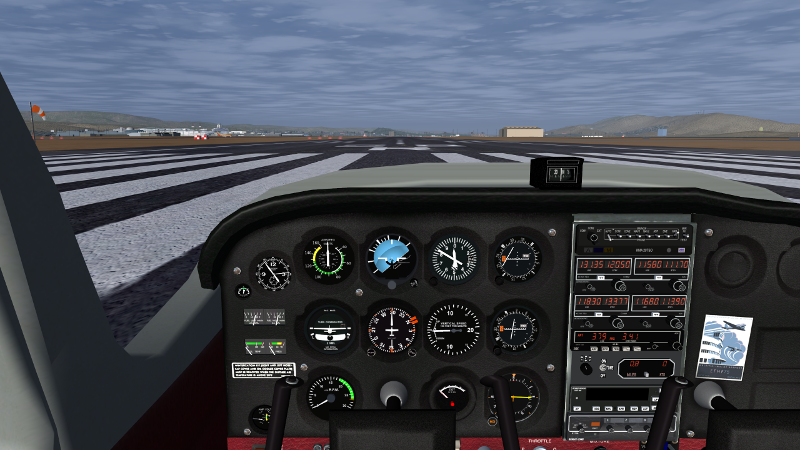
\includegraphics[clip,width=12.5cm]{img/ksfo}
}}
\smallskip
 \noindent

\iflanguage{english}{
Fig.\,3: Ready for takeoff: \textit{Waiting at the default startup position at San Francisco Intl., KSFO.}
}{}
\iflanguage{french}{
Fig.\,3 : Par\'{e} \`{a} d\'{e}coller : \textit{en attente \`{a} la position de d\'{e}marrage par d\'{e}faut de l'a\'{e}roport de San Francisco Intl., KSFO.}
}{}
\medskip

\iflanguage{english}{
Before you can run \FlightGear{}, you need to set a couple of environment variables:
}{}
\iflanguage{french}{
Avant de pouvoir d\'{e}marrer \FlightGear{}, vous devez d\'{e}finir deux variables d'environnement :
}{}

\begin{itemize}
\iflanguage{english}{
\item You must add \texttt{/usr/local/share/FlightGear/lib} to your \texttt{LD\_LIBRARY\_PATH}
\item \texttt{FG\_ROOT} must be set to the data directory of your \FlightGear{} installation. e.g. \texttt{/usr/local/share/FlightGear/data}.
\item \texttt{FG\_SCENERY} should be a list of scenery directories, separated by '':''. This works like \texttt{PATH} when searching for scenery.
e.g. \texttt{\$FG\_ROOT/Scenery:\$FG\_ROOT/WorldScenery}.
}{}

\iflanguage{french}{
\item Vous devez ajouter \texttt{/usr/local/share/FlightGear/lib} \`{a} votre \texttt{LD\_LIBRARY\_PATH}
\item \texttt{FG\_ROOT} doit \^{e}tre param\'{e}tr\'{e} pour pointer vers le r\'{e}pertoire contenant les donn\'{e}es de votre installation de  \FlightGear{}, par exemple : \texttt{/usr/local/share/FlightGear/data}.
\item \texttt{FG\_SCENERY} doit \^{e}tre une liste de r\'{e}pertoires de sc\`{e}nes, s\'{e}par\'{e}s par '':''. Ce fonctionnement est semblable \`{a} celui de \texttt{PATH} lorsqu'on recherche des sc\`{e}nes.
par exemple : \texttt{\$FG\_ROOT/Scenery:\$FG\_ROOT/WorldScenery}.
}{}

\end{itemize}

\noindent
\iflanguage{english}{
To add these in the Bourne shell (and compatibles):
}{}
\iflanguage{french}{
Pour les ajouter dans le Bourne shell (et compatibles) :
}{}
\begin{verbatim}
LD_LIBRARY_PATH=/usr/local/share/FlightGear/lib:$LD_LIBRARY_PATH
export LD_LIBRARY_PATH
FG_HOME=/usr/local/share/FlightGear
export FG_HOME
FG_ROOT=/usr/local/share/FlightGear/data
export FG_ROOT
FG_SCENERY=$FG_ROOT/Scenery:$FG_ROOT/WorldScenery
export FG_SCENERY
\end{verbatim}
\noindent

\iflanguage{english}{
 or in C shell (and compatibles):
}{}
\iflanguage{french}{
 ou en C shell (et compatibles) :
}{}

\begin{verbatim}
setenv LD_LIBRARY_PATH=\
  /usr/local/share/FlightGear/lib:$LD_LIBRARY_PATH
setenv FG_HOME=/usr/local/share/FlightGear
setenv FG_ROOT=/usr/local/share/FlightGear/data
setenv FG_SCENERY=\
  $FG_HOME/Scenery:$FG_ROOT/Scenery:$FG_ROOT/WorldScenery
\end{verbatim}

\iflanguage{english}{
 Once you have these environment variables set up, simply start \FlightGear{} by running
}{}
\iflanguage{french}{
 Une fois que ces variables d'environnement ont \'{e}t\'{e} param\'{e}tr\'{e}es, d\'{e}marrez tout simplement \FlightGear{} en utilisant la commande 
}{}
\texttt{fgfs -$ $-option1 -$ $-option2\dots}
\medskip
\iflanguage{english}{
Command-line options are described in Chapter~\ref{options}.
}{}
\iflanguage{french}{
Les options de ligne de commande sont d\'{e}crites dans le chapitre~\ref{options}.
}{}

%%%%%%%%%%%%%%%%%%%%%%%%%%%%%%%%%%%%%%%%%%%%%%%%%%%%%%%%%%%%%%%%%%%%%%%%%%%%%%%%%%%%%%%%%%%%%%%
\iflanguage{english}{
\section{Launching the simulator under Windows}\index{Launching Flightgear!Windows}\index{Starting Flightgear!Windows}
}{}
\iflanguage{french}{
\section{D\'{e}marrer le simulateur sous Windows}\index{D\'{e}marrer Flightgear!Windows}\index{D\'{e}marrer Flightgear!Windows}
}{}
%%%%%%%%%%%%%%%%%%%%%%%%%%%%%%%%%%%%%%%%%%%%%%%%%%%%%%%%%%%%%%%%%%%%%%%%%%%%%%%%%%%%%%%%%%%%%%%

\iflanguage{english}{
The pre-built windows binaries come complete with a graphical wizard to start \FlightGear{}. Simply double-click on the \texttt{FlightGear Launcher} Start Menu item, or the icon on the Desktop. The launcher allows you to select your aircraft, the start airport and runway, time of day, current weather, and lots
of other settings.
}{}
\iflanguage{french}{
Les binaires pr\'{e}-compil\'{e}s pour Windows sont livr\'{e}s avec un assistant graphique pour d\'{e}marrer \FlightGear{}. Cliquez tout simplement sur l'\'{e}l\'{e}ment \texttt{FlightGear Launcher} du menu D\'{e}marrer, ou double-cliquez sur l'ic\^{o}ne pr\'{e}sente sur le Bureau. L'assistant vous permet de choisir votre a\'{e}ronef, l'a\'{e}roport de d\'{e}marrage et la piste, l'heure du jour, la m\'{e}t\'{e}o en cours, et de nombreux autres param\`{e}tres.
}{}

 \centerline{\fbox{
\includegraphics[clip,width=12.5cm]{launcher}
}}
\smallskip
\noindent

\iflanguage{english}{
Fig.\,4: \textit{The FlightGear Launcher}
}{}
\iflanguage{french}{
Fig.\,4: \textit{L'assistant de d\'{e}marrage de FlightGear}
}{}

\medskip
\iflanguage{english}{
The first time your run it, you will be asked to set your \texttt{FG\_ROOT} variable
(normally \texttt{c:$\backslash$Program Files$\backslash$FlightGear$\backslash$data}) and \texttt{FG\_SCENERY}.
This should be a list of the directories where you have installed scenery, typically
\texttt{c:$\backslash$Program Files$\backslash$FlightGear$\backslash$data$\backslash$Scenery}.

If you set invalid values or change your scenery directories later, you can
change the settings by pressing the ''Prev'' button from the first page of
the launcher.
}{}
\iflanguage{french}{
La premi\`{e}re fois que vous le lancerez, il vous sera demand\'{e} de param\'{e}trer vos variables \texttt{FG\_ROOT}
(g\'{e}n\'{e}ralement \texttt{c:$\backslash$Program Files$\backslash$FlightGear$\backslash$data}) et \texttt{FG\_SCENERY}.
Ce cette derni\`{e}re variable doit contenir une liste de r\'{e}pertoire(s) o\`{u} vous avez install\'{e} des sc\`{e}nes,
typiquement :

\texttt{c:$\backslash$Program Files$\backslash$FlightGear$\backslash$data$\backslash$Scenery}.

Si vous indiquez des valeurs incorrectes ou si vous modifiez les r\'{e}pertoires de vos sc\`{e}nes apr\`{e}s coup, vous pourrez
corriger ces valeurs et appuyant sur le bouton ''Pr\'{e}c\'{e}dent'' \`{a} partir de la premi\`{e}re page de l'assistant.
}{}

\iflanguage{english}{
\subsection{Launching from the command line}
}{}
\iflanguage{french}{
\subsection{Lancement \`{a} partir de la ligne de commande}
}{}

\iflanguage{english}{
Alternatively, you can run FlightGear from the command line. To do this, you
need to set up the \texttt{FG\_ROOT} and \texttt{FG\_SCENERY} environment
variables manually.

Open a command shell, change to the directory where your binary resides
(typically something like
\texttt{c:$\backslash$Program Files$\backslash$FlightGear$\backslash$bin$\backslash$Win32}),
set the environment variables by typing
}{}
\iflanguage{french}{
Alternativement, vous pouvez d\'{e}marrer FlightGear \`{a} partir de la ligne de commande. Pour cela, vous devez param\'{e}trer
les variables d'environnement \texttt{FG\_ROOT} et \texttt{FG\_SCENERY} manuellement.

Ouvrez une invite de commandes, placez-vous dans le r\'{e}pertoire o\`{u} sont positionn\'{e}s vos binaires (g\'{e}n\'{e}ralement quelque chose comme \texttt{c:$\backslash$Program Files$\backslash$FlightGear$\backslash$bin$\backslash$Win32}), puis param\'{e}trez les variables d'environnement en tapant :
}{}

\medskip

\begin{verbatim}
SET FG_HOME="c:\Program Files\FlightGear"
SET FG_ROOT="c:\Program Files\FlightGear\data"
SET FG_SCENERY="c:\Program Files\FlightGear\data\Scenery"
\end{verbatim}
\medskip

\noindent
\iflanguage{english}{
 and invoke \FlightGear{} (within the same Command shell, as environment
 settings are only valid locally within the same shell) via
}{}
\iflanguage{french}{
 et d\'{e}marrez \FlightGear{} (dans la m\^{e}me fen\^{e}tre d'invite de commandes, car les variables d'environnement sont valides
uniquement localement au sein de la m\^{e}me invite de commandes) par l'interm\'{e}diaire de la commande :
}{}
\medskip

\texttt{fgfs -$ $-option1 -$ $-option2\dots}
\medskip
\iflanguage{english}{
Command-line options are described in Chapter~\ref{options}.
Of course, you can create a batch file with a Windows text editor (like notepad)
using the lines above.
For maximum performance it is recommended that you to minimize (iconize) the
text output window while running \FlightGear{}.
}{}
\iflanguage{french}{
Les options de ligne de commande sont d\'{e}crites dans le chapitre~\ref{options}.
Naturellement, vous pouvez cr\'{e}er un fichier \textit{batch} avec un \'{e}diteur de texte Windows (comme le bloc-notes) contenant les lignes ci-dessus.
Pour obtenir les meilleures performances \`{a} l'ex\'{e}cution, il est recommand\'{e} de r\'{e}duire (ic\^{o}nifier) la fen\^{e}tre de sortie pendant que \FlightGear{} est en fonctionnement. 
}{}


%%%%%%%%%%%%%%%%%%%%%%%%%%%%%%%%%%%%%%%%%%%%%%%%%%%%%%%%%%%%%%%%%%%%%%%%%%%%%%%%%%%%%%%%%%%%%%%
\iflanguage{english}{
\section{Launching the simulator under Mac OS X}\index{Launching Flightgear!Mac OS X}\index{Starting Flightgear!Mac OS X}
}{}
\iflanguage{french}{
\section{D\'{e}marrer le simulateur sous Mac OS X}\index{D\'{e}marrer Flightgear!Mac OS X}\index{D\'{e}marrer Flightgear!Mac OS X}
}{}
%%%%%%%%%%%%%%%%%%%%%%%%%%%%%%%%%%%%%%%%%%%%%%%%%%%%%%%%%%%%%%%%%%%%%%%%%%%%%%%%%%%%%%%%%%%%%%%
\iflanguage{english}{
The prebuilt binary package for Mac OS X comes with the GUI launcher. Simply double-click the \FlightGear{} icon on /Applications folder shows up the GUI launcher window as shown in Fig. 5. The launcher allows you to :

\begin{itemize}
\item Select an aircraft and an airport
\item Enable/Disable automatic scenery download (using \TerraSync{})
\item Enable/Disable the Navigation Map (Atlas)
\item Launch \FlightGear{}
\end{itemize}

The following sections describe the use of these features.
}{}

\iflanguage{french}{
Le paquetage de binaires pr\'{e}-compil\'{e}s pour Mac OS X est livr\'{e} avec un assistant en mode graphique. Double-cliquez simplement sur l'ic\^{o}ne \FlightGear{} dans le dossier /Applications pour lancer la fen\^{e}tre GUI launcher comme d\'{e}montr\'{e} \`{a} la Fig. 5. L'assistant vous permet :

\begin{itemize}
\item de choisir un a\'{e}ronef et un a\'{e}roport
\item d'activer/d\'{e}sactiver le t\'{e}l\'{e}chargement automatique des sc\`{e}nes (en utilisant \TerraSync{})
\item d'activer/d\'{e}sactiver la carte de navigation (Atlas)
\item de d\'{e}marrer \FlightGear{}
\end{itemize}

Les sections suivantes d\'{e}crivent l'utilisation de ces fonctionnalit\'{e}s.
}{}
\smallskip
\centerline{\fbox{
\includegraphics[clip,width=12.5cm]{img/maclauncher}
}}
\smallskip
\noindent
\iflanguage{english}{
Fig.\,5: \textit{The GUI Launcher for Mac OS X} \label{fig:maclauncher}
}{}
\iflanguage{french}{
Fig.\,5: \textit{L'assistant graphique pour Mac OS X} \label{fig:maclauncher}
}{}

\medskip

\iflanguage{english}{
\subsection{Selecting an aircraft and an airport}
At the launcher window, you can select an aircraft and an airport by clicking gear buttons at the right end of the airport/aircraft name. The thumbnail image of a selected aircraft will show up at the image panel on the window. The airport that you select here will be the starting point of your flight. \FlightGear{} uses ICAO 4-letter airport code, which is composed with one or two prefix letters followed by a two or three letter airport code. For example, the ICAO code for San Francisco International Airport is KSFO. ``K'' in this case is the prefix for The United States, and SFO is the airport code for San Francisco International Airport. You can use \textit{Advanced features >> Position} or \textit{Aircraft} tab to find an airport or an aircraft.
}{}
\iflanguage{french}{
\subsection{Choisir un a\'{e}ronef et un a\'{e}roport}
Dans la fen\^{e}tre de l'assistant, vous pouvez choisir un a\'{e}ronef et un a\'{e}roport en cliquant sur les boutons situ\'{e}s \`{a} droite du nom de l'a\'{e}roport/a\'{e}ronef. L'image miniature de l'a\'{e}ronef s\'{e}lectionn\'{e} s'affichera dans le panneau image de la fen\^{e}tre. L'a\'{e}roport que vous choisissez ici sera le point de d\'{e}part de votre vol. \FlightGear{} utilise les codes a\'{e}roport \`{a} quatre lettres de l'OACI, qui se compose d'une ou deux lettres de pr\'{e}fixe, suivies de une ou deux lettres correspondant au code a\'{e}roport. Par exemple, le code OACI de l'a\'{e}roport international de San Francisco est KSFO. Dans cet exemple, ``K'' est le pr\'{e}fixe pour les Etats-Unis, et SFO est le code a\'{e}roport pour l'a\'{e}roport international de San Francisco. Vous pouvez utiliser l'onglet \textit{Fonctionnalit\'{e}s avanc\'{e}es >> Position} ou \textit{A\'{e}ronef} pour trouver un a\'{e}roport ou un a\'{e}ronef.
}{}

\iflanguage{english}{
\subsection{Enabling on-the-fly scenery downloading}
By checking \textit{Download scenery on the fly} at the launcher window, the scenery data will be downloaded while you're flying using \TerraSync{}. The scenery downloader will install the scenery data into \\
}{}
\iflanguage{french}{
\subsection{Activer le t\'{e}l\'{e}chargement des sc\`{e}nes \`{a} la vol\'{e}e}
En activant \textit{T\'{e}l\'{e}charger les sc\`{e}nes \`{a} la vol\`{e}e} dans la fen\^{e}tre de l'assistant, les donn\'{e}es des sc\`{e}nes seront t\'{e}l\'{e}charg\'{e}es pendant que vous volez grace \'{a} \TerraSync{}. L'outil de t\'{e}l\'{e}chargement des scenes installera ces donn\'{e}es dans le r\'{e}pertoire \\
}{}

\texttt{/Applications/FlightGear.app/Contents/Resouces/data/Scenery-Terrasync}. 

\iflanguage{english}{
\subsection{Enabling Navigation Map (Atlas)}
The Mac version of \FlightGear{} includes Atlas, the navigation map that helps your flight plan, for your convenience. Checking this option will automatically launch Atlas when you start the flight. You don't have to specify any Atlas options. The GUI launcher will specify these for you.
}{}
\iflanguage{french}{
\subsection{Activer la carte de navigation (Atlas)}
La version Mac de \FlightGear{} comprend Atlas, la carte de navigation qui vous aide \`{a} suivre votre plan de vol, pour votre confort. L'activation de cette option lancera automatiquement Atlas lorsque vous d\'{e}marrerez votre vol. Vous n'avez pas besoin de sp\'{e}cifier d'options Atlas. L'assistant graphique les pr\'{e}cisera pour vous.
}{}

\iflanguage{english}{
\subsection{Launching FlightGear - the simulator}
Clicking \textit{Start Flight} button at the launcher window opens up another window - the FlightGear main window. \FlightGear{} immediately starts loading tons of data required for simulation. It may take a while on slower machines to load everything.
}{}
\iflanguage{french}{
\subsection{D\'{e}marrer FlightGear - le simulateur}
Cliquer sur le bouton \textit{D\'{e}marrer le vol} dans la fen\^{e}tre de l'assistant ouvre une nouvelle fen\^{e}tre - la fen\^{e}tre principale de FlightGear. \FlightGear{} d\'{e}marre imm\'{e}diatement le chargement des tonnes de donn\'{e}es n\'{e}cessaires pour la simulation. Le temps de chargement peut \^{e}tre un peu long sur des machines lentes.
}{}

\iflanguage{english}{
\subsection{Advanced Features}
\FlightGear{} has many features and options that you can specify at launch time. Some of these are not changeable from the menu in the \FlightGear{} main window. To enable / disable these features, click the triangle-shaped button at the left-bottom of the launcher window. This displays the advanced features tabs. All settings are saved so you don't have to respecify them.
}{}

\iflanguage{french}{
\subsection{Fonctionnalit\'{e}s avanc\'{e}es}
\FlightGear{} poss\`{e}de de nombreuses fonctionnalit\'{e}s et options que vous pouvez sp\'{e}cifier lors du d\'{e}marrage. Quelques-unes d'entre elles ne peuvent pas \^{e}tre modifi\'{e}es \`{a} partir du menu de la fen\^{e}tre principale de \FlightGear{}. Pour activer/d\'{e}sactiver ces fonctionnalit\'{e}s, cliquez sur le bouton en forme de triangle dans l'angle inf\'{e}rieur gauche de la fen\^{e}tre de l'assistant. Ceci affiche l'onglet fonctionnalit\'{e}s avanc\'{e}es. Tous les param\`{e}tres sont sauvegard\'{e}s de mani\`{e}re \`{a} ce que vous n'ayez pas \`{a} les resp\'{e}cifier \`{a} chaque fois.
}{}

\iflanguage{english}{
\subsubsection{General, Features, and Rendering tabs}
These tabs let you specify some of \FlightGear{} options:
\begin{itemize}
\item \textbf{Save preferences on exit:} lets \FlightGear{} save preferences that you changed from the menu in the \FlightGear{} (fgfs) main window will be saved to \\ \texttt{\$HOME/.fgfs/autosave.xml}.
\item \textbf{Control:} specifies the control device you will use in \FlightGear{}. \textit{auto, joystick, mouse, and keyboard} are available. You can leave it as \textit{auto} unless you really want to change it manually.
\item \textbf{Unit:} specifies the unit used in \FlightGear{}. \textit{feet} and \textit{meters} are available.
\item \textbf{Time of day:} specifies the time of day. Available options are \textit{real, dawn, morning, noon, afternoon, dusk, evening, and midnight}.
\item \textbf{Season:} specifies the season of \FlightGear{} world. You can choose either summer or winter.
\item \textbf{Sound:} disabling this will cut all the sound in FlightGear.
\item \textbf{Instrumental panel:} specifies if 2D panel is drawn from the beginning. You can also enable/disable the 2D panel from \FlightGear{} menu.
\item \textbf{Random objects:} specifies whether \FlightGear{} draws random objects or not.
\item \textbf{AI models:} specifies whether \FlightGear{} handles AI aircraft and ships.
\item \textbf{Clock never advances:} specifies whether the clock advances in \FlightGear{} or not.
\item \textbf{No fuel consumption:} makes aircraft consume no fuel while it's flying.
\item \textbf{Start in a frozen state:} starts \FlightGear{} with frozen state. it does not seem working at this moment.
\item \textbf{Display HUD:} displays HUD at the beginning, I guess. You can turn HUD on/off by pressing 'h' while you are flying.
\item \textbf{3D HUD:} enables 3D HUD if an selected aircraft supports it.
\item \textbf{Real weather fetch:} enables fetching real weather condition using METAR.
\item \textbf{Horizon effect:} enables horizon effect.
\item \textbf{Clouds:} enables drawing clouds.
\item \textbf{3D clouds:} enables drawing 3D clouds. You need to enable 3D clouds by checking \textit{3D cloud} from the \textit{View >> Rendering option} on the \FlightGear{} simulator window. 
\item \textbf{Turbulence:} specifies the strength of turbulence. 0.0 is calm and 1.0 is severe. You need to specify value from 0.0 through 1.0
\item \textbf{Visibility:} specifies the visibility in meter. You can specify 5000 or less if \FlightGear{} runs slow on your machine.
\item \textbf{Fullscreen mode:} enabling this will launch \FlightGear{} as full-screen mode.
\item \textbf{Window size:} specifies the size of \FlightGear{} window. It will be ignored when full-screen mode is enabled.
\item \textbf{Sky blending:} enables or disables \FlightGear{} to blend the sky depending on time and surrounding environment. DO NOT disable this option, or \FlightGear{} crashes.
\item \textbf{Textures:} enables or disables textures on runways, buildings, and scenery objects. Disabling this will give you some more fps, effective especially on G4 Macs.
\item \textbf{Wireframe:} lets \FlightGear{} draw wire-frames so you can see how the world of \FlightGear{} is drawn. This should be enabled only for debug / development purpose.
\item \textbf{Fog:} specifies how fog is drawn. \textit{disable, fastest, nicest} are available.
\end{itemize}
}{}

\iflanguage{french}{
\subsubsection{Onglets G\'{e}n\'{e}ralit\'{e}s, Fonctionnalit\'{e}s et Rendu}
Ces onglets vous permettent de d\'{e}finir certaines options de \FlightGear{} :
\begin{itemize}
\item \textbf{Sauvegarder les pr\'{e}f\'{e}rences \`{a} la fermeture :} permet \`{a} \FlightGear{} de sauvegarder les pr\'{e}f\'{e}rences que vous avez modifi\'{e}es \`{a} partir du menu dans la fen\^{e}tre principale de \FlightGear{} (fgfs) vers le fichier \\ \texttt{\$HOME/.fgfs/autosave.xml}.
\item \textbf{Contr\^{o}les :} pr\'{e}cise le moyen de contr\^{o}le que vous utiliserez dans \FlightGear{}. \textit{auto, joystick, souris et clavier} sont disponibles. Vous pouvez conserver ce param\`{e}tre en mode \textit{auto} sauf si vous tenez \`{a} le param\'{e}trer manuellement.
\item \textbf{Unit\'{e}s :} d\'{e}finit l'unit\'{e} utilis\'{e}e dans \FlightGear{}. Les \textit{pieds} et les \textit{m\`{e}tres} sont disponibles.
\item \textbf{Heure du jour :} fixe l'heure du jour. Les options disponibles sont \textit{r\'{e}elle, aube, matin, midi, apr\`{e}s-midi, cr\'{e}puscule, soir et minuit}.
\item \textbf{Saison :} d\'{e}finit la saison du monde \FlightGear{}. Vous pouvez choisir \'{e}t\'{e} ou hiver.
\item \textbf{Son :} la d\'{e}sactivation de cette option coupera le son dans FlightGear.
\item \textbf{Panneaux d'instruments :} pr\'{e}cise si un panneau 2D est activ\'{e} par d\'{e}faut. Vous pouvez \'{e}galement activer/d\'{e}sactiver le panneau 2D \`{a} partir du menu \FlightGear{}.
\item \textbf{Objets al\'{e}atoires :} pr\'{e}cise si \FlightGear{} affichera des objets al\'{e}atoires ou non.
\item \textbf{Mod\`{e}les IA :} pr\'{e}cise si \FlightGear{} g\`{e}rera les a\'{e}ronefs et navires IA.
\item \textbf{L'horloge n'avance jamais :} d\'{e}finit si l'horloge avance dans \FlightGear{} ou non.
\item \textbf{Pas de consommation de carburant :} laisse l'avion ne consommer aucun carburant lorsqu'il vole.
\item \textbf{D\'{e}marrer dans un \'{e}tat fig\'{e} :} d\'{e}marre \FlightGear{} dans un \'{e}tat fig\'{e}. Cette option a l'air de ne pas fonctionner actuellement.
\item \textbf{Activer l'affichage t\^{e}te haute (HUD) :} affiche le HUD au d\'{e}marrage, je pense. Vous pouvez activer/d\'{e}sactiver le HUD en appuyant sur 'h' lorsque vous volez.
\item \textbf{HUD 3D :} active le HUD 3D si un avion s\'{e}lectionn\'{e} le prend en charge.
\item \textbf{M\'{e}t\'{e}o r\'{e}elle :} active la r\'{e}cup\'{e}ration des conditions m\'{e}t\'{e}o r\'{e}elles en utilisant les METAR.
\item \textbf{Effet de l'horizon :} active l'effet de l'horizon.
\item \textbf{Nuages :} active l'affichage des nuages.
\item \textbf{Nuages 3D :} active l'affichage des nuages 3D. Vous devrez activer les nuages 3D en activant la case \textit{Nuages 3D} dans le menu \textit{Affichage >> Options de rendu} dans la fen\^{e}tre du simulateur \FlightGear{}. 
\item \textbf{Turbulence :} pr\'{e}cise la force des turbulences en vol. 0.0 est calme et 1.0 est forte. Vous devez sp\'{e}cifier une valeur allant de 0.0 \`{a} 1.0.
\item \textbf{Visibilit\'{e} :} sp\'{e}cifie la visibilit\'{e} en m\`{e}tres. Vous pouvez donner une valeur de 5 000 ou moins si \FlightGear{} tourne lentement sur votre machine.
\item \textbf{Mode plein \'{e}cran :} l'activation de ce param\`{e}tre lancera \FlightGear{} en mode plein \'{e}cran.
\item \textbf{Taille de la fen\^{e}tre :} d\'{e}finit la taille de la fen\^{e}tre \FlightGear{}. Sera ignor\'{e} si le mode plein \'{e}cran est activ\'{e}.
\item \textbf{Fondu du ciel :} active ou d\'{e}sactive le fondu du ciel dans \FlightGear{} en fonction du temps et de l'environnement proche. NE DESACTIVEZ PAS cette option, sous peine de voir \FlightGear{} dysfonctionner.
\item \textbf{Textures :} active ou d\'{e}sactive les textures sur les pistes, les immeubles et les objets des sc\`{e}nes. La d\'{e}sactivation vous donnera quelques images par seconde en plus, sp\'{e}cialement sur les Macs G4.
\item \textbf{Fil de fer :} demande \`{a} \FlightGear{} de dessiner le monde en fils de fer, de telle sorte que vous puissiez visualiser la mani\`{e}re dont le monde de \FlightGear{} est rendu. Ceci ne devrait \^{e}tre activ\'{e} que pour des besoins de d\'{e}bogage ou de d\'{e}veloppement.
\item \textbf{Brouillard :} pr\'{e}cise la mani\`{e}re dont le brouillard est rendu. \textit{d\'{e}sactiv\'{e}, plus rapide, plus beau} sont les options disponibles.
\end{itemize}
}{}

\iflanguage{english}{
\subsubsection{Favorite tab}
Favorite list provides a means of preserving a named set of current options like a book mark of a web browser. To save the current set of options, press ``+'' button on the top window or at the bottom of the Favorite tab. Once favorites are added, You can switch from one configuration to another by double-clicking a row in the table view in the Favorite tab. Pressing ``-'' button (or delete key) on a favorite in the table view deletes the selected favorite.
}{}
\iflanguage{french}{
\subsubsection{Onglet Favoris}
La liste des favoris offre un moyen de conserver un \'{e}tat nomm\'{e} des options actuelles, \`{a} la fa\c{c}on du marque-pages d'un navigateur Internet. Pour sauvegarder l'\'{e}tat actuel des options, appuyez sur le bouton ``+'' dans le haut de la fen\^{e}tre ou en-bas de l'onglet Favoris. Une fois que les favoris ont \'{e}t\'{e} ajout\'{e}s, vous pouvez basculer d'une configuration \`{a} l'autre en double-cliquant sur une ligne du tableau dans l'onglet Favoris. L'appui sur le bouton ``-'' (ou sur la touche suppression) sur un favori dans le tableau efface le favori s\'{e}lectionn\'{e}.
}{}

\subsubsection{Position}
\iflanguage{english}{
You can find airports or aircraft carriers by searching with a keyword into the filter text area. Available keywords are:
}{}
\iflanguage{french}{
Vous pouvez trouver des a\'{e}roports ou des porte-avions en cherchant en utilisant une recherche par mot-cl\'{e} dans la zone de texte filtre. Les mots-cl\'{e}s disponibles sont :
}{}

\begin{itemize}
\iflanguage{english}{
\item For airports:
	\begin {itemize} 
	\item a part of airport name (e.g. international, ranch, or civil),
	\item country name (such as Japan, USA, or France) if available,
	\item location name (such as city or county or U.S. state abbrev. if available),
	\item IATA code (such as SFO, LAX, HND) if available,
	\item ICAO code (such as KSFO, KLAX, RJTT) - works on all airports.
	\end{itemize}
\item For aircraft carriers:
	\begin{itemize}
	\item carrier name (Nimitz or Eisenhower),
	\item ``carrier''.
	\end{itemize}
}{}
\iflanguage{french}{
\item Pour les a\'{e}roports :
	\begin {itemize} 
	\item une partie du nom de l'a\'{e}roport (par exemple : international, ranch, ou civil),
	\item le nom du pays (comme Japon, USA, ou France) si connu,
	\item le nom de l'emplacement (comme la ville ou le nom abbr\'{e}g\'{e} de l'\'{e}tat aux Etats-Unis),
	\item code IATA (comme SFO, LAX, HND) si disponible,
	\item code OACI (comme KSFO, KLAX, RJTT) - fonctionne pour tous les a\'{e}roports.
	\end{itemize}
\item Pour les porte-avions :
	\begin{itemize}
	\item nom du porte-avions (Nimitz ou Eisenhower),
	\item ``carrier''.
	\end{itemize}
}{}

\end{itemize}

\iflanguage{english}{
Airports and carriers that match the keyword are shown at the table view below the filter text area. The airport name at the upper pane is synchronized with the currently selected airport or carrier. You can also open this tab by clicking the gear button at the right end of airport name on the top pane.
When you choose an airport, available runways show up at the ``runway'' pop-up button. You can choose a runway or leave it as ``default.''
}{}
\iflanguage{french}{
Les a\'{e}roports et les porte-avions qui correspondent au mot-cl\'{e} sont affich\'{e}s dans la vue du tableau sous la zone de texte filtre. Vous pouvez \'{e}galement ouvrir cet onglet en cliquant sur le bouton situ\'{e} \`{a} l'extr\'{e}mit\'{e} droite du nom de l'a\'{e}roport sur le panneau sup\'{e}rieur.
Lorsque vous choisissez un a\'{e}roport, les pistes disponibles s'affichent dans le bouton pop-up ``piste''. Vous pouvez choisir une piste ou le laisser sur ``d\'{e}faut.''
}{}

\iflanguage{english}{
\subsubsection{Aircraft tab}
You can find aircraft by searching with a keyword into the filter text area. Available keywords are:
}{}
\iflanguage{french}{
\subsubsection{Onglet A\'{e}ronefs}
Vous pouvez trouver les a\'{e}ronefs en cherchant avec un mot cl\'{e} dans la zone de texte filtre. Les mot-cl\'{e}s disponibles sont :
}{}

\iflanguage{english}{
\begin{itemize}
\item a part of aircraft name (e.g. c172, zero, shinden)
\item configuration file name without -set.xml (e.g. a6m2, p51d)
\item fdm (Flight Dynamics Model) name (e.g. yasim, jsb)
\item status (e.g. alpha, beta, production, development)
\end{itemize}
A list of aircraft that match the keyword shows up at the table view below the filter text area. The aircraft name at the upper pane is synchronized with the currently selected aircraft. You can also open this tab by clicking the gear button at the right end of aircraft name on the top pane.

If you want to find more aircraft data from the internet, click ``Get Aircraft'' button at the bottom of the Aircraft tab. It opens a web browser to lead you to the Aircraft Links page on \textit{FlightGear Mac OS X} web site. You can visit some links there and download an aircraft you want. Once an aircraft is downloaded, open ``Others'' tab to install it. 

If you encounter some weird behavior in searching aircraft, removing a cache file for aircraft database might solve your problem. Open \\ \texttt{/Applications/Utilities/Terminal.app} and type the following commands to remove the cache file:
}{}
\iflanguage{french}{
\begin{itemize}
\item une partie du nom de l'a\'{e}ronef (par exemple : c172, zero, shinden)
\item le nom d'un fichier de configuration sans le -set.xml (par exemple : a6m2, p51d)
\item le nom du FDM (Mod\`{e}le de dynamique de vol) (par exemple : yasim, jsb)
\item le statut (par exemple : alpha, beta, production, d\'{e}veloppement)
\end{itemize}
Une liste des a\'{e}ronefs correspondant au mot cl\'{e} s'affichent dans la vue du tableau sous la zone de texte filtre. Le nom d'a\'{e}ronef sur le panneau sup\'{e}rieur est synchronis\'{e} avec l'a\'{e}ronef actuellement s\'{e}lectionn\'{e}. Vous pouvez \'{e}galement ouvrir cet onglet en cliquant sur le bouton situ\'{e} \`{a} l'extr\'{e}mit\'{e} droite du nom de l'avion sur le panneau sup\'{e}rieur.

Si vous voulez trouver plus d'a\'{e}ronefs \`{a} partir d'Internet, cliquez sur le boutou ``Obtenir des a\'{e}ronefs'' en bas de l'onglet A\'{e}ronefs. Ceci ouvrira un navigateur pour vous mener \`{a} la page Liens A\'{e}ronefs sur le site Internet \textit{FlightGear Mac OS X}. Vous pouvez consulter certains liens qui s'y trouvent et t\'{e}l\'{e}charger l'a\'{e}ronef que vous souhaitez. Une fois que l'a\'{e}ronef est t\'{e}l\'{e}charg\'{e}, ouvrez l'onglet ``Autres'' pour l'installer. 

Si vous constatez un comportement anormal lorsque vous recherchez un a\'{e}ronef, supprimer un fichier de cache de la base de donn\'{e}es des a\'{e}ronefs peut r\'{e}soudre votre probl\`{e}me. Ouvrez \\ \texttt{/Applications/Utilities/Terminal.app} et tapez les commandes suivantes pour supprimer le fichier de cache :
}{}

\begin{verbatim}
  cd /Applications/FlightGear.app/Contents/Resources
  rm AircraftCache.rb
\end{verbatim}

\medskip
\iflanguage{english}{
Note that you must not launch \FlightGear{} from mounted disk image of a prebuilt binary package since the folder in the mounted disk image is read-only, which prevents you from installing any add-on data. Vou need to install \FlightGear{} by copying the \FlightGear{} icon from the mounted disk image to \texttt{/Applications} folder.
}{}
\iflanguage{french}{
Notez que vous ne devez pas lancer \FlightGear{} \`{a} partir de l'image disque d'un paquetage binaire pr\'{e}compil\'{e} car le r\'{e}pertoire de l'image disque mont\'{e}e est en lecture seule, ce qui vous emp\^{e}che d'installer toute donn\'{e}e ajout\'{e}e. Vous devez installer \FlightGear{} en copiant l'ic\^{o}ne \FlightGear{} depuis l'image disque mont\'{e}e vers le r\'{e}pertoire \texttt{/Applications}.
}{}

\iflanguage{english}{
\subsubsection{Network tab}
This tab contains two network features of \FlightGear{}. One is multi-player mode and another is FGCOM (a voice ATC). To enable multi-player mode, specify the followings:
\begin{itemize}
\item \textbf{Enable Multiplay:} enables or disables multi-player mode. Enabling this will open a new browser window to show the map on a multi player server.
\item \textbf{Callsign:} specifies the name shown in the map. Username must contain only alphabet letters, numbers, underscores, and dots. \FlightGear{} will exit when you specify a call sign with invalid characters. A user name with 8 or more characters will be truncated into the first 7 characters. 
\item \textbf{Server:} specifies the server to connect. \texttt{mpserver02.flightgear.org} is available at the time of writing this.
\item \textbf{Your Mac:} specifies your Mac's IP address. Usually the launcher detects the address automatically. If something is wrong with network connection, clear this text field.
\item \textbf{Port:} must be 5000
\end{itemize}

FGCOM enables you to make a real voice communication using radio setting. You can talk at a selected radio frequency (COM1) while pressing space bar. You can listen to some other player's talking in the frequency if some others are using the same frequency and you are in range. The options available for FGCOM are listed below:

\begin{itemize}
\item \textbf{Enable FGCOM in Multi Player mode:} specifies if you use FGCOM when Multiplay is enabled.
\item \textbf{FGCOM Server:} specifies a VOIP server.
\end{itemize}

For further instructions on FGCOM, and Multiplay, please see Chapter \ref{features}.
}{}

\iflanguage{french}{
\subsubsection{Onglet r\'{e}seau}
Cet onglet contient deux fonctionnalit\'{e}s r\'{e}seau de \FlightGear{}. L'une est le mode multijoueurs et l'autre est FGCOM (un syst\`{e}me de contr\^{o}le a\'{e}rien vocal). Pour activer le mode multijoueurs, pr\'{e}cisez les items suivants :
\begin{itemize}
\item \textbf{Activer le mode multijoueurs :} active ou d\'{e}sactive le mode multijoueurs. L'activation ouvrira une nouvelle fen\^{e}tre du navigateur pour afficher la carte sur un serveur multijoueurs.
\item \textbf{Indicatif :} pr\'{e}cise le nom affich\'{e} sur la carte. Un nom d'utilisateur peut contenir des lettres de l'alphabet, des nombres, des tirets-bas (\textit{underscores}) et des points. \FlightGear{} se terminera si vous pr\'{e}cisez un indicatif avec des caract\`{e}res invalides. Un nom d'utilisateur contenant 8 caract\`{e}res ou plus sera tronqu\'{e} avec les seuls 7 premiers caract\`{e}res. 
\item \textbf{Serveur :} pr\'{e}cise le serveur auquel se connecter. \texttt{mpserver02.flightgear.org} est disponible \`{a} l'heure de l'\'{e}criture de ce document.
\item \textbf{Votre Mac :} d\'{e}finit l'adresse IP de votre Mac. G\'{e}n\'{e}ralement, l'assistant d\'{e}tecte l'adresse de mani\`{e}re automatique. Si quelque chose n'est pas exact avec votre connection r\'{e}seau, effacez le contenu de ce champ texte.
\item \textbf{Port :} doit \^{e}tre \'{e}gal \`{a} 5000.
\end{itemize}

FGCOM vous permet d'effectuer une v\'{e}ritable communication audio en utilisant des param\`{e}tres radio. Vous pouvez parler sur une fr\'{e}quence radio pr\'{e}cise (COM1) en appuyant sur la barre d'espace. Vous pouvez \'{e}coutez d'autres joueurs parlant sur la fr\'{e}quence si d'autres joueurs sont sur cette fr\'{e}quence et que vous \^{e}tes \`{a} leur port\'{e}e. Les options pour FGCOM sont list\'{e}es ci-dessous :

\begin{itemize}
\item \textbf{Active FGCOM en mode multijoueurs :} indique si vous utilisez FGCOM lorsque le mode multijoueurs est activ\'{e}.
\item \textbf{Serveur FGCOM :} pr\'{e}cise un serveur VOIP.
\end{itemize}

Des informations compl\'{e}mentaires concernant FGCOM et le mode multijoueurs sont disponibles au chapitre \ref{features}.
}{}

\iflanguage{english}{
\subsubsection{Others tab}
You can specify any options other than aircraft, airport, and the options shown in the launcher. Entering space-separated options as shown in Figure 11 will pass additional options to \FlightGear{}. You can see all available options by pressing ``View Options.'' Some options might cause \FlightGear{} crash. If you encounter such crashes with a specific option, please let us know.

To install additional aircraft and scenery data, press "Install Add-on Data." You can specify multiple files and/or folders to install to the \FlightGear{} data folder. Acceptable file types are:
\begin{itemize}
\item zip
\item tar
\item tar.gz
\item tar.bz2
\item folder
\item 7zip (only if 7zip is installed)
\end{itemize}

You will see the message window when all the data is successfully installed, otherwise error message will show up. You can select both aircraft and scenery data at the same time. If you select an archived file that does not contain aircraft files, it will be extracted into the data folder, but will be ignored. When you finish installing new aircraft, you can select the aircraft on the ``Aircraft'' tab.
}{}
\iflanguage{french}{
\subsubsection{Onglet Autres}
Vous pouvez pr\'{e}ciser toutes les options autres que a\'{e}ronef, a\'{e}roport et les options affich\'{e}es dans l'assistant. En entrant des options s\'{e}par\'{e}es par des espaces comme pr\'{e}sent\'{e} \`{a} la Figure 11, vous passerez des options additionnelles \`{a} \FlightGear{}. Vous pouvez voir toutes les options disponibles en appuyant sur ``Voir Options.'' Certaines options peuvent faire dysfonctionner \FlightGear{}. Si vous rencontrez de tels dysfonctionnements avec une option particuli\`{e}re, merci de nous le signaler.

Pour installer des a\'{e}ronefs et des sc\`{e}nes additionnelles, appuyez sur "Installer des donn\'{e}es additionnelles." Vous pouvez pr\'{e}ciser les fichiers ou r\'{e}pertoires multiples \`{a} installer dans le r\'{e}pertoire des donn\'{e}es \FlightGear{}. Les types de fichiers accept\'{e}s sont :
\begin{itemize}
\item zip
\item tar
\item tar.gz
\item tar.bz2
\item dossier
\item 7zip (seulement si 7zip est install\'{e})
\end{itemize}

Vous verrez la fen\^{e}tre d'information lorsque toutes les donn\'{e}es ont \'{e}t\'{e} correctement install\'{e}es, dans le cas contraire les messages d'erreurs y seront affich\'{e}s. Vous pouvez choisir des donn\'{e}es d'a\'{e}ronefs et de sc\`{e}nes en m\^{e}me temps. Si vous choisissez un fichier archiv\'{e} qui ne contient pas de fichiers d'a\'{e}ronefs, il sera extrait dans le r\'{e}pertoire des donn\'{e}es, mais sera ignor\'{e}. Lorsque vous aurez termin\'{e} l'installation d'un nouvel a\'{e}ronef, vous pouvez choisir l'a\'{e}ronef concern\'{e} dans l'onglet ``A\'{e}ronefs''.
}{}

\iflanguage{english}{
\subsection{Launching from the command line}
You can also launch the simulator from the command line on Mac OS X. To do so, open Terminal.app (located at \texttt{/Applications/Utilities}) and type the following commands:
}{}
\iflanguage{french}{
\subsection{D\'{e}marrage \`{a} partir de la ligne de commande}
Vous pouvez \'{e}galement d\'{e}marrer le simulateur \`{a} partir de la ligne de commande sur Mac OS X. Pour le faire, ouvrez Terminal.app (situ\'{e} dans \texttt{/Applications/Utilitaires}) et tapez les commandes suivantes :
}{}

\begin{verbatim}
  cd /Applications/FlightGear.app/Contents/Resources
  ./fgfs --option1 --option2 ....
\end{verbatim}

\iflanguage{english}{
See chapter \ref{options} for detail information on command line options. Unlike the other platforms, you don't have to manually specify the environment variables such as FG\_ROOT and FG\_SCENERY as long as you use a prebuilt binary package.
}{}
\iflanguage{french}{
Reportez-vous au chapitre \ref{options} pour obtenir plus d'informations d\'{e}taill\'{e}es sur les options en ligne de commande. Contrairement aux autres plate-formes, vous n'avez pas besoin de pr\'{e}ciser manuellement les variables d'environnement comme FG\_ROOT et FG\_SCENERY tant que vous utilisez un paquetage binaire pr\'{e}compil\'{e}.
}{}

%%%%%%%%%%%%%%%%%%%%%%%%%%%%%%%%%%%%%%%%%%%%%%%%%%%%%%%%%%%%%%%%%%%%%%%%%%%%%%%%%%%%%%%%%%%%%%%
\section{Command line parameters\label{options}}\index{command line options}
%%%%%%%%%%%%%%%%%%%%%%%%%%%%%%%%%%%%%%%%%%%%%%%%%%%%%%%%%%%%%%%%%%%%%%%%%%%%%%%%%%%%%%%%%%%%%%%
Following is a complete list and short description of the numerous \Index{command line options}
available for \FlightGear{}. Most of these options are exposed through the \FlightGear{} launcher delivered with the
Windows binaries.

If you have options you re-use continually, you can create a preferences file
containing a set of command-line options that will be set automatically. You
can create the file with any text editor (notepad, emacs, vi, if you like).

\begin{itemize}
\item On Unix systems (including Mac OS X), put the command line options in a
file called \texttt{.fgfsrc}\index{.fgfsrc} in your home directory.

\item On Windows, put the command line options in a file called \texttt{system.fgfsrc}
\index{system.fgfsrc} in the \texttt{FG\_ROOT} directory (e.g. \texttt{c:$\backslash$Program Files$\backslash$FlightGear$\backslash$data}).
\end{itemize}

%%%%%%%%%%%%%%%%%%%%%%%%%%%%%%%%%%%%%%%%%%%%%%%%%%%%%%%%%%%%%%%%%%%%%%%%%%%%%%%%%%%%%%%%%%%%%%%
\subsection{General Options}\index{options!general}\label{generaloptions}
%%%%%%%%%%%%%%%%%%%%%%%%%%%%%%%%%%%%%%%%%%%%%%%%%%%%%%%%%%%%%%%%%%%%%%%%%%%%%%%%%%%%%%%%%%%%%%%
\begin{itemize}
\item{\texttt{-$ $-help}}

  Display the most relevant command line options.

\item{\texttt{-$ $-help} \texttt{-$ $-verbose}}

  Display all command line options.

\item{\texttt{-$ $-language={\it code}}}

  Select the language for this session. e.g. pl, nl, it, fr, en, de.

\item{\texttt{-$ $-version} }

Display the current \FlightGear{} version.

\item{\texttt{-$ $-fg-root={\it path}}}

  Tells \FlightGear{} where to look for its root data files if you
  didn't compile it with the \Index{default settings}.

\item{\texttt{-$ $-fg-scenery={\it path}}}

  Allows specification of a path to the base scenery path
  \index{scenery directory!path}, in case scenery is not at the default
  position under \texttt{\$FG\underline{~}ROOT/Scenery}; this might
  be especially useful in case you have scenery on a CD-ROM.

\item{\texttt{-$ $-enable-save-on-exit}, \texttt{-$ $-disable-save-on-exit}}

  Enable or disable saving of user-preferences on exit from the simulator.

\item{\texttt{-$ $-enable-freeze}, \texttt{-$ $-disable-freeze}}

  Control whether \FlightGear{} starts paused or not. Defaults to not paused.

\item{\texttt{-$ $-control={\it mode}}}

  Specify your primary \Index{control mode} (\Index{\texttt{joystick}},  \texttt{keyboard},
  \texttt{mouse}) Defaults to \Index{joystick}.

\item{\texttt{-$ $-enable-auto-coordination}, \texttt{-$ $-disable-auto-coordination}}

  Switches \Index{auto-co-ordination} between aileron and rudder on/off. Auto-coordination
  is recommended for users without rudder pedals or a `twist' joystick. Defaults to off.

\item{\texttt{-$ $-browser-app={\it path}}}

  Specify location of your web browser. E.g:
  \texttt{-$ $-browser-app=}\\
  \texttt{``C:$\backslash$Program~Files$\backslash$Internet~Explorer$\backslash$iexplore.exe''}
  (Note the `` '' because of the spaces!).

\item{\texttt{-$ $-config={\it path}}}

  Load additional properties from the given path. E.g:\\
  \texttt{-$ $-config=./Aircraft/X15-set.xml}

\item{\texttt{-$ $-units-feet}}

  Use feet as the unit of measurement.

\item{\texttt{-$ $-units-meters}}
  Use meters as the unit of measurement.
\end{itemize}
%%%%%%%%%%%%%%%%%%%%%%%%%%%%%%%%%%%%%%%%%%%%%%%%%%%%%%%%%%%%%%%%%%%%%%%%%%%%%%%%%%%%%%%%%%%%%%%
\subsection{Features}\index{options!features}
%%%%%%%%%%%%%%%%%%%%%%%%%%%%%%%%%%%%%%%%%%%%%%%%%%%%%%%%%%%%%%%%%%%%%%%%%%%%%%%%%%%%%%%%%%%%%%%
\begin{itemize}

\item{\texttt{-$ $-enable-ai-models}, \texttt{-$ $-disable-ai-models}}

  Enable or disable other aircraft/AI-models in the simulator.

\item{\texttt{-$ $-ai-scenario={\it name}}}

  Enable a specific AI scenario (e.g. \texttt{-$ $-ai-scenario=vinson-demo}). May be used multiple times.

\item{\texttt{-$ $-enable-random-objects}, \texttt{-$ $-disable-random-objects}}

  Enable, disable random scenery objects (buildings/trees). Enabled by default.

\end{itemize}

%%%%%%%%%%%%%%%%%%%%%%%%%%%%%%%%%%%%%%%%%%%%%%%%%%%%%%%%%%%%%%%%%%%%%%%%%%%%%%%%%%%%%%%%%%%%%%%
\subsection{Sound}\index{options!sound}
%%%%%%%%%%%%%%%%%%%%%%%%%%%%%%%%%%%%%%%%%%%%%%%%%%%%%%%%%%%%%%%%%%%%%%%%%%%%%%%%%%%%%%%%%%%%%%%
\begin{itemize}
\item{\texttt{-$ $-enable-sound}, \texttt{-$ $-disable-sound}}

  Enable or disable sound.

\item{\texttt{-$ $-show-sound-devices}}

  Show the available sound devices.

\item{\texttt{-$ $-sound-device={\it device}}}

  Specify the sound device to use for audio.

\item{\texttt{-$ $-enable-intro-music}, \texttt{-$ $-disable-intro-music}}

  Enable or disable playing an audio sample when \FlightGear{} starts up.

\end{itemize}

%%%%%%%%%%%%%%%%%%%%%%%%%%%%%%%%%%%%%%%%%%%%%%%%%%%%%%%%%%%%%%%%%%%%%%%%%%%%%%%%%%%%%%%%%%%%%%%
\subsection{Aircraft\index{aircraft!selection}}\index{options!aircraft}
%%%%%%%%%%%%%%%%%%%%%%%%%%%%%%%%%%%%%%%%%%%%%%%%%%%%%%%%%%%%%%%%%%%%%%%%%%%%%%%%%%%%%%%%%%%%%%%

\begin{itemize}
\item{\texttt{-$ $-aircraft={\it aircraft}}}

Load the specified aircraft, for example: \texttt{-$ $-aircraft=c172p}. For available choices
check the directory \texttt{\$FG\underline{~}ROOT/Aircraft}, and look for files ending in \texttt{``-set.xml''}.
When specifying the aircraft, drop the \texttt{``-set.xml''} from the filename. Alternatively, use
the \texttt{-$ $-show-aircraft} option described below to list the available aircraft. For information
on downloading additional aircraft, see Section \ref{install_aircraft}.

\item{\texttt{-$ $-show-aircraft}}

Print a sorted list of the currently available aircraft types.

\item{\texttt{-$ $-min-status={\it status}}}

Display only those aircraft with a specified minimum declared status, one of
\texttt{alpha}, \texttt{beta}, \texttt{early-production}, \texttt{production}. For use with \texttt{-$ $-show-aircraft}.

\item{\texttt{-$ $-aircraft-dir={\it PATH}}}

Aircraft directory relative to the executable location. Defaults to \texttt{\$FG\underline{~}ROOT/Aircraft}.

\item{\texttt{-$ $-vehicle={\it name of aircraft definition file}}}

Synonym for \texttt{-$ $-aircraft}.

\item{\texttt{-$ $-livery={\it Name}}}

Set the aircraft livery.

\end{itemize}

%%%%%%%%%%%%%%%%%%%%%%%%%%%%%%%%%%%%%%%%%%%%%%%%%%%%%%%%%%%%%%%%%%%%%%%%%%%%%%%%%%%%%%%%%%%%%%%
\subsection{Flight model\index{flight dynamics model}}\index{options!flight model}\label{flight dynamics model}
%%%%%%%%%%%%%%%%%%%%%%%%%%%%%%%%%%%%%%%%%%%%%%%%%%%%%%%%%%%%%%%%%%%%%%%%%%%%%%%%%%%%%%%%%%%%%%%
\begin{itemize}
\item{\texttt{-$ $-fdm={\it abcd}}}

Select the core \Index{flight model}. Options are \texttt{jsb}, \texttt{larcsim}, \texttt{yasim},
\texttt{magic}, \texttt{balloon}, \texttt{external}, \texttt{pipe}, \texttt{ada}, \texttt{null}.
This option can normally be ignored, as the \texttt{-$ $-aircraft} option will set the FDM correctly.

\item{\texttt{-$ $-aero={\it aircraft}}}

Specifies the \Index{aircraft aeronautical model} to load. This option can normally be ignored, as
the \texttt{-$ $-aircraft} option will set the aircraft model correctly.

\item{\texttt{-$ $-model-hz={\it n}}}

Run the Flight Dynamics Model with this rate (iterations per second).

\item{\texttt{-$ $-speed={\it n}}}

Run the Flight Dynamics Model this much faster than real time.

\item{\texttt{-$ $-trim}, \texttt{-$ $-notrim}}

Trim (or not) when initializing JSBSim. Defaults to trim.

\item{\texttt{-$ $-on-ground}, \texttt{-$ $-in-air}}

Start up at ground level (default), or in the air. If specifying \texttt{-$ $-in-air} you
must also set an initial altitude using \texttt{-$ $-altitude}, and may also want to set
an initial velocity with \texttt{-$ $-vc}. Note that some aircraft (notably the X15) must
be started in mid-air.

\item{\texttt{-$ $-enable-fuel-freeze}, \texttt{-$ $-disable-fuel-freeze}}

Control whether fuel state is constant (e.g. frozen) or consumed normally (default).

\end{itemize}

%%%%%%%%%%%%%%%%%%%%%%%%%%%%%%%%%%%%%%%%%%%%%%%%%%%%%%%%%%%%%%%%%%%%%%%%%%%%%%%%%%%%%%%%%%%%%%%
\subsection{Initial Position and Orientation\label{aiportid}}\index{options!initial position}\index{options!orientation}
%%%%%%%%%%%%%%%%%%%%%%%%%%%%%%%%%%%%%%%%%%%%%%%%%%%%%%%%%%%%%%%%%%%%%%%%%%%%%%%%%%%%%%%%%%%%%%%
\begin{itemize}
\item{\texttt{-$ $-airport={\it ABCD}}}

Start at a specific \Index{airport}. The airport is specified by its ICAO code, e.g. \texttt{-$ $-airport=KJFK} for
JFK airport in New York. For US airport without an ICAO code, try prefixing the 3 character code
with `K'.

\item{\texttt{-$ $-parking-id={\it ABCD}}}

Start at a specific parking spot on the airport.

\item{\texttt{-$ $-runway={\it NNN}}}

Start at the threshold of a specific runway (e.g. 28L). If no runway or parking ID is
specified, a runway facing into the wind will be chosen for takeoff.

\item{\texttt{-$ $-vor={\it ABCD}}, \texttt{-$ $-ndb={\it ABCD}}, \texttt{-$ $-fix={\it ABCD}}}

Set the starting position relative to a VOR, NDB or FIX. Useful for practising approaches.

\item{\texttt{-$ $-carrier={\it NAME}}}

Start on an aircraft carrier. See \ref{carrier} for details of carrier operations.

\item{\texttt{-$ $-parkpos={\it NAME}}}

Start at a particular parking position on the carrier. Must be used with \texttt{-$ $-carrier}.
Defaults to a catapult launch position.

\item{\texttt{-$ $-offset-distance={\it nm}}, \texttt{-$ $-offset-azimuth={\it deg}}}

Start at a particular distance and heading from a position set using \texttt{-$ $-airport},
\texttt{-$ $-vor}, \texttt{-$ $-ndb}, \texttt{-$ $-fix}, \texttt{-$ $-carrier}.

\item{\texttt{-$ $-lon={\it degrees}}, \texttt{-$ $-lat={\it degrees}}}

\index{longitude}\index{latitude}\index{Startup longitude}\index{Startup latitude}
Start at a particular longitude and latitude, in decimal degrees (south, west negative).

\item{\texttt{-$ $-altitude={\it feet}}}

Start at specific altitude. Implies \texttt{-$ $-in-air}. Altitude is specified in feet unless you
also select \texttt{-$ $-units-meters}, in which case altitude is in meters. You may also want to set
an initial velocity with \texttt{-$ $-vc} to avoid stalling immediately.

\item{\texttt{-$ $-heading={\it degrees}}, \texttt{-$ $-roll={\it degrees}}, \texttt{-$ $-pitch={\it degrees}}}

Set the initial \Index{orientation} of the aircraft. All values default to 0 - heading North, in straight and level flight.

\item{\texttt{-$ $-uBody={\it X}}, \texttt{-$ $-vBody={\it Y}}, \texttt{-$ $-wBody={\it Z}}}

Set the initial speed along the X, Y and Z axes. Speed is in feet per second unless you
also select \texttt{-$ $-units-meters}, in which case altitude is in meters per second.

\item{\texttt{-$ $-vNorth={\it N}}, \texttt{-$ $-vEast={\it E}}, \texttt{-$ $-vDown={\it D}}}

Set the initial speed along the South-North, West-East and vertical axes. Speed is in feet per second unless you
also select \texttt{-$ $-units-meters}, in which case altitude is in meters per second.

\item{\texttt{-$ $-vc={\it knots}}, \texttt{-$ $-mach={\it num}}}

Set the initial airspeed in knots or as a Mach number. Useful if setting \texttt{-$ $-altitude}, unless you want to stall immediately!

\item{\texttt{-$ $-glideslope={\it degrees}}, \texttt{-$ $-roc={\it fpm}}}

Set the initial glide slope angle in degrees or as a climb rate in feet per minute. May be positive or negative.

\end{itemize}

%%%%%%%%%%%%%%%%%%%%%%%%%%%%%%%%%%%%%%%%%%%%%%%%%%%%%%%%%%%%%%%%%%%%%%%%%%%%%%%%%%%%%%%%%%%%%%%
\subsection{Environment Options\index{options!environment}}
%%%%%%%%%%%%%%%%%%%%%%%%%%%%%%%%%%%%%%%%%%%%%%%%%%%%%%%%%%%%%%%%%%%%%%%%%%%%%%%%%%%%%%%%%%%%%%%
\begin{itemize}
\item{\texttt{-$ $-ceiling={\it FT\underline{~}ASL[:THICKNESS\underline{~}FT]}}}

Sets an overcase ceiling at a particular height, and with an optional thickness (defaults to 2000ft).

\item{\texttt{-$ $-enable-real-weather-fetch}, \texttt{-$ $-disable-real-weather-fetch}}

Control whether real-time weather information is downloaded and used.

\item{\texttt{-$ $-metar={\it METAR STRING}}}

Use a specific METAR string, e.g. \texttt{-$ $-metar="XXXX 012345Z 00000KT 99SM CLR 19/M01 A2992"}. The METAR may
be specified in most common formats (US, European). Incompatible with \texttt{-$ $-enable-real-weather-fetch}.

\item{\texttt{-$ $-random-wind}}

Sets random wind direction and strength.

\item{\texttt{-$ $-turbulence={\it n}}}

Sets turbulence from completely calm (0.0) to severe (1.0).


\item{\texttt{-$ $-wind={\it DIR@SPEED}}}

Specify the surface wind. Direction is in degrees, and speed in knots. Values may be specified as a range
by using a colon separator; e.g. \texttt{-$ $-wind=180:220@10:15}.

\item{\texttt{-$ $-season={\it param}}}

Sets the simulated season. Valid parameters are \texttt{summer} (default), \texttt{winter}.

\item{\texttt{-$ $-visibility={\it meters}}, \texttt{-$ $-visibility-miles={\it miles}}}

\end{itemize}

%%%%%%%%%%%%%%%%%%%%%%%%%%%%%%%%%%%%%%%%%%%%%%%%%%%%%%%%%%%%%%%%%%%%%%%%%%%%%%%%%%%%%%%%%%%%%%%
\subsection{Rendering Options\index{options!rendering}}
%%%%%%%%%%%%%%%%%%%%%%%%%%%%%%%%%%%%%%%%%%%%%%%%%%%%%%%%%%%%%%%%%%%%%%%%%%%%%%%%%%%%%%%%%%%%%%%
\begin{itemize}

\item{\texttt{-$ $-aspect-ratio-multiplier={\it N}}}

Set a multiplier for the display aspect ratio.

\item{\texttt{-$ $-bpp={\it depth}}}

Specify the bits per pixel.


\item{\texttt{-$ $-enable-clouds}, \texttt{-$ $-disable-clouds}}

Enable (default) or disable \Index{cloud layers}.

\item{\texttt{-$ $-enable-clouds3d}, \texttt{-$ $-disable-clouds3d}}

Enable (default), disable \Index{3D clouds}. Very pretty, but depend on your graphics card supporting
GLSL Shaders, which some older, or less powerful graphics cards do not.

\item{\texttt{-$ $-enable-distance-attenuation}, \texttt{-$ $-disable-distance-attenuation}}

Enable or disable more realistic runway and approach light attenuation.

\item{\texttt{-$ $-enable-enhanced-lighting}, \texttt{-$ $-disable-enhanced-lighting}}

Enable or disable more realistic runway and approach lights.

\item{\texttt{-$ $-enable-fullscreen}, \texttt{-$ $-disable-fullscreen}}

Enable, disable (default) full screen mode.

\item{\texttt{-$ $-enable-game-mode}, \texttt{-$ $-disable-game-mode}}

Enable or disable \Index{full screen display} for 3DFX graphics cards.

\item{\texttt{-$ $-enable-horizon-effect}, \texttt{-$ $-disable-horizon-effect}}

Enable (default), disable celestial body growth illusion near the horizon.

\item{\texttt{-$ $-enable-mouse-pointer}, \texttt{-$ $-disable-mouse-pointer}}

Enable, disable (default) extra \Index{mouse pointer}. Useful in full screen mode for old Voodoo based cards.

\item{\texttt{-$ $-enable-panel}, \texttt{-$ $-disable-panel}}

Enable (default) the \Index{instrument panel}.

\item{\texttt{-$ $-enable-skyblend}, \texttt{-$ $-disable-skyblend}}

Enable (default), disable fogging/haze.

\item{\texttt{-$ $-enable-specular-highlight}, \texttt{-$ $-disable-specular-highlight}}

Enable (default), disable specular highlights.

\item{\texttt{-$ $-enable-splash-screen}, \texttt{-$ $-disable-splash-screen}}

Enable or disable (default) the rotating 3DFX logo when the accelerator board gets initialized (3DFX only).

\item{\texttt{-$ $-enable-textures}, \texttt{-$ $-disable-textures}}

Enable (default), disable use of textures.

\item{\texttt{-$ $-enable-wireframe}, \texttt{-$ $-disable-wireframe}}

Enable, disable (default) display of wireframes. If you want to know what the world of
\FlightGear{} looks like internally, try this!\index{wireframe}

\item{\texttt{-$ $-fog-disable}, \texttt{-$ $-fog-fastest}, \texttt{-$ $-fog-nicest}}

Set the fog level. To cut down the rendering efforts, distant regions vanish in \Index{fog} by default.
If you disable \Index{fog} you'll see farther, but your frame rates will drop. Using \texttt{-$ $-fog-fastest}
will display a less realistic fog, by increase \Index{frame rate}. Default is \texttt{-$ $-fog-nicest}.

\item{\texttt{-$ $-fov={\it degrees}}}

Sets the \Index{field of view} in degrees. Default is 55.0.

\item{\texttt{-$ $-geometry={\it WWWxHHH}}}

Defines the window/screen resolution. E.g. \texttt{-$ $-geometry=1024x768}.\index{window size}.

\item{\texttt{-$ $-shading-smooth}, \texttt{-$ $-shading-flat}}

Use smooth shading (default), or flat shading which is faster but less pretty.

\item{\texttt{-$ $-texture-filtering={\it N}}}

Configure anisotropic texture filtering. Values are 1 (default), 2, 4, 8 or 16.

\item{\texttt{-$ $-view-offset={\it xxx}}}

Allows setting the default forward view direction as an offset from straight ahead.
Possible values are \texttt{LEFT, RIGHT, CENTER}, or a specific number of degrees.
Useful for multi-window display.\index{offset}
\end{itemize}

%%%%%%%%%%%%%%%%%%%%%%%%%%%%%%%%%%%%%%%%%%%%%%%%%%%%%%%%%%%%%%%%%%%%%%%%%%%%%%%%%%%%%%%%%%%%%%%
\subsection{HUD Options\index{HUD}\index{options!HUD}}
%%%%%%%%%%%%%%%%%%%%%%%%%%%%%%%%%%%%%%%%%%%%%%%%%%%%%%%%%%%%%%%%%%%%%%%%%%%%%%%%%%%%%%%%%%%%%%%
\begin{itemize}
\item{\texttt{-$ $-enable-anti-alias-hud}, \texttt{-$ $-disable-anti-alias-hud}}

Control whether the \Index{HUD} (\textbf{H}ead \textbf{U}p  \textbf{D}isplay) is shown anti-aliased.

\item{\texttt{-$ $-enable-hud}, \texttt{-$ $-disable-hud}}

Control whether the HUD is displayed. Defaults to disabled.

\item{\texttt{-$ $-enable-hud-3d}, \texttt{-$ $-disable-hud-3d}}

Control whether the 3D HUD is displayed.

\item{\texttt{-$ $-hud-culled}, \texttt{-$ $-hud-tris}}

Display the percentage of triangles culled, or the number of triangles rendered in the HUD. Mainly
of interest to graphics developers.

\end{itemize}

%%%%%%%%%%%%%%%%%%%%%%%%%%%%%%%%%%%%%%%%%%%%%%%%%%%%%%%%%%%%%%%%%%%%%%%%%%%%%%%%%%%%%%%%%%%%%%%
\subsection{Aircraft System Options\index{Avionics}\index{options!Aircraft Systems}}
%%%%%%%%%%%%%%%%%%%%%%%%%%%%%%%%%%%%%%%%%%%%%%%%%%%%%%%%%%%%%%%%%%%%%%%%%%%%%%%%%%%%%%%%%%%%%%%
\begin{itemize}
\item{\texttt{-$ $-adf={\it [radial:]frequency}}}

Set the ADF frequency and radial.

\item{\texttt{-$ $-com1={\it frequency}}, \texttt{-$ $-com2={\it frequency}}}

Set the COM1/COM2 radio frequency.

\item{\texttt{-$ $-dme={\it {nav1|nav2|frequency}}}}

Set the DME to NAV1, NAV2, or a specific frequency and radial.

\item{\texttt{-$ $-failure={\it system}}}

Fail a specific aircraft system. Valid systems are \texttt{pitot}, \texttt{static},
\texttt{vacuum}, \texttt{electrical}. Specify multiple times to fail multiple systems.

\item{\texttt{-$ $-nav1={\it [radial:]frequency}}, \texttt{-$ $-nav2={\it [radial:]frequency}}}

Set the NAV1/NAV2 radio frequency and radial.

\end{itemize}

%%%%%%%%%%%%%%%%%%%%%%%%%%%%%%%%%%%%%%%%%%%%%%%%%%%%%%%%%%%%%%%%%%%%%%%%%%%%%%%%%%%%%%%%%%%%%%%
\subsection{Time Options}\index{time options}\index{options!time}
%%%%%%%%%%%%%%%%%%%%%%%%%%%%%%%%%%%%%%%%%%%%%%%%%%%%%%%%%%%%%%%%%%%%%%%%%%%%%%%%%%%%%%%%%%%%%%%
\begin{itemize}

\item{\texttt{-$ $-enable-clock-freeze}, \texttt{-$ $-disable-clock-freeze}}

Control whether time advances normally or is frozen.

\item{\texttt{-$ $-start-date-gmt={\it yyyy:mm:dd:hh:mm:ss}},
\texttt{-$ $-start-date-lat={\it yyyy:mm:dd:hh:mm:ss}}, \texttt{-$ $-start-date-sys={\it yyyy:mm:dd:hh:mm:ss}}}

Specify the exact startup time/date. The three functions differ in that they
take either Greenwich Mean Time, the local time of your virtual flight, or
your computer system's local time as the reference point.

Incompatible with \texttt{-$ $-time-match-local}, \texttt{-$ $-time-match-real}.

\item{\texttt{-$ $-time-match-local}, \texttt{-$ $-time-match-real}}

{-$ $-time-match-real}, is default: Simulator time is read from the system clock, and
is used as is. When your virtual flight is in the same timezone as where your computer
is located, this may be desirable, because the clocks are synchronized. However,
when you fly in a different part of the world, it may not be the case, because there
is a number of hours difference, between the position of your computer and the position of your
virtual flight.

The option {-$ $-time-match-local} takes care of this by computing the timezone
difference between your real world time zone and the position of your virtual
flight, and local clocks are synchronized.

Incompatible with \texttt{-$ $-start-date-gmt}, \texttt{-$ $-start-date-lat}, \texttt{-$ $-start-date-sys}.

\item{\texttt{-$ $-time-offset={\it [+-]hh:mm:ss}}}

Specify a time offset relative to one of the time options above.

\item{\texttt{-$ $-timeofday={\it param}}}

Set the time of day. Valid parameters are \texttt{real}, \texttt{dawn}, \texttt{morning},
\texttt{noon}, \texttt{afternoon}, \texttt{dusk}, \texttt{evening}, \texttt{midnight}.

\end{itemize}

%%%%%%%%%%%%%%%%%%%%%%%%%%%%%%%%%%%%%%%%%%%%%%%%%%%%%%%%%%%%%%%%%%%%%%%%%%%%%%%%%%%%%%%%%%%%%%%
\subsection{Network Options}\index{network options}\index{options!network}
%%%%%%%%%%%%%%%%%%%%%%%%%%%%%%%%%%%%%%%%%%%%%%%%%%%%%%%%%%%%%%%%%%%%%%%%%%%%%%%%%%%%%%%%%%%%%%%
\begin{itemize}
\item{\texttt{-$ $-multiplay={\it dir,Hz,host,port}}, \texttt{-$ $-callsign={\it ABCD}}}

Set multiplay options and aircraft call-sign. See Section \ref{multiplayer}.

\item{\texttt{-$ $-httpd={\it port}}, \texttt{-$ $-telnet={\it port}}}

Enable \Index{http server} or \Index{telnet server} on the specified port to provide
access to the property tree.

\item{\texttt{-$ $-jpg-httpd={\it port}}}

Enable screen shot http server on the specified port.

\item{\texttt{-$ $-proxy={\it [user:password@]host:port}}}

Specify a proxy server to use.

\end{itemize}
%%%%%%%%%%%%%%%%%%%%%%%%%%%%%%%%%%%%%%%%%%%%%%%%%%%%%%%%%%%%%%%%%%%%%%%%%%%%%%%%%%%%%%%%%%%%%%%
\subsection{Route/Waypoint Options}\index{options!route}\index{options!waypoint}
%%%%%%%%%%%%%%%%%%%%%%%%%%%%%%%%%%%%%%%%%%%%%%%%%%%%%%%%%%%%%%%%%%%%%%%%%%%%%%%%%%%%%%%%%%%%%%%
\begin{itemize}
\item{\texttt{-$ $-wp={\it ID[@alt]}}}

  Allows specifying a waypoint for the GC autopilot; it is possible to
  specify multiple waypoints (i.e. a route) via multiple instances of
  this command.

\item{\texttt{-$ $-flight-plan={\it [file]}}}

  This is more comfortable if you have several waypoints. You can
  specify a file to read them from.
\end{itemize}

NB: These options are rather geared to the advanced user who knows what he is doing.

%%%%%%%%%%%%%%%%%%%%%%%%%%%%%%%%%%%%%%%%%%%%%%%%%%%%%%%%%%%%%%%%%%%%%%%%%%%%%%%%%%%%%%%%%%%%%%%
\subsection{IO Options}\index{options!IO}
%%%%%%%%%%%%%%%%%%%%%%%%%%%%%%%%%%%%%%%%%%%%%%%%%%%%%%%%%%%%%%%%%%%%%%%%%%%%%%%%%%%%%%%%%%%%%%%

More detailed descriptions of the various IO parameters can be found in the README.IO file 
within the Docs directory of your \FlightGear{} installation.

\begin{itemize}

\item{\texttt{-$ $-atlas={\it params}}}

  Open connection using the Atlas protocol (used by Atlas and TerraSync).

\item{\texttt{-$ $-atcsim={\it params}}}

  Open connection using the ATC Sim protocol (atc610x).

\item{\texttt{-$ $-AV400={\it params}}}

  Open connection to drive a Garmin 196/296 series GPS

\item{\texttt{-$ $-AV400Sim={\it params}}}

  Open connection to drive a Garmin 400 series GPS

\item{\texttt{-$ $-generic={\it params}}}

  Open connection using the Generic (XML-defined) protocol.

\item{\texttt{-$ $-garmin={\it params}}}

  Open connection using the Garmin GPS protocol.

\item{\texttt{-$ $-joyclient={\it params}}}

  Open connection to an Agwagon joystick.

\item{\texttt{-$ $-jsclient={\it params}}}

  Open connection to a remote joystick.

\item{\texttt{-$ $-native-ctrls={\it params}}}

  Open connection using the FG native Controls protocol.

\item{\texttt{-$ $-native-fdm={\it params}}}

  Open connection using the FG Native FDM protocol.

\item{\texttt{-$ $-native-gui={\it params}}}

  Open connection using the FG Native GUI protocol.

\item{\texttt{-$ $-native={\it params}}}

  Open connection using the FG Native protocol.

\item{\texttt{-$ $-nmea={\it params}}}

  Open connection using the NMEA protocol.

\item{\texttt{-$ $-opengc={\it params}}}

  Open connection using the OpenGC protocol.

\item{\texttt{-$ $-props={\it params}}}

  Open connection using the interactive property manager.

\item{\texttt{-$ $-pve={\it params}}}

  Open connection using the PVE protocol.

\item{\texttt{-$ $-ray={\it params}}}

  Open connection using the RayWoodworth motion chair protocol.

\item{\texttt{-$ $-rul={\it params}}}

  Open connection using the RUL protocol.

\end{itemize}

%%%%%%%%%%%%%%%%%%%%%%%%%%%%%%%%%%%%%%%%%%%%%%%%%%%%%%%%%%%%%%%%%%%%%%%%%%%%%%%%%%%%%%%%%%%%%%%
\subsection{Debugging options}\index{options!debugging}
%%%%%%%%%%%%%%%%%%%%%%%%%%%%%%%%%%%%%%%%%%%%%%%%%%%%%%%%%%%%%%%%%%%%%%%%%%%%%%%%%%%%%%%%%%%%%%%
\begin{itemize}

\item{\texttt{-$ $-enable-fpe}}

Enable abort on a Floating Point Exception. 

\item{\texttt{-$ $-fgviewer}}

Instead of loading the entire simulator, load a lightweight OSG viewer. Useful for checking aircraft
models.

\item{\texttt{-$ $-log-level={\it LEVEL}}}

Set the logging level. Valid values are \texttt{bulk}, \texttt{debug}, \texttt{info}, \texttt{warn}, \texttt{alert}.

\item{\texttt{-$ $-prop:[type:]name=value}}

Set property \texttt{name} to \texttt{value}

Example: \texttt{-$ $-prop:/engines/engine[0]/running=true} starts the simulator with running engines.

Another example:

\texttt{-$ $-aircraft=c172p}\\
\texttt{-$ $-prop:/consumables/fuels/tank[0]/level-gal=10}\\
\texttt{-$ $-prop:/consumables/fuels/tank[1]/level-gal=10}\\

fills the Cessna for a short flight. You may optionally specific
the property type (\texttt{double}, \texttt{string}, \texttt{boolean}).

\item{\texttt{-$ $-trace-read={\it params}}}

Trace the reads for a property; multiple instances are allowed.

\item{\texttt{-$ $-trace-write={\it params}}}

Trace the writes for a property; multiple instances are allowed.
\end{itemize}



%%%%%%%%%%%%%%%%%%%%%%%%%%%%%%%%%%%%%%%%%%%%%%%%%%%%%%%%%%%%%%%%%%%%%%%%%%%%%%%%%%%%%%%%%%%%%%%
\section{Joystick support\label{joysticksupp}}\index{joystick}
%%%%%%%%%%%%%%%%%%%%%%%%%%%%%%%%%%%%%%%%%%%%%%%%%%%%%%%%%%%%%%%%%%%%%%%%%%%%%%%%%%%%%%%%%%%%%%%
Could you imagine a pilot in his or her Cessna controlling the machine with
a keyboard alone? For getting the proper feeling of flight you will need a
joystick/yoke plus rudder pedals, right? However, the combination of
numerous types of \Index{joystick}s, flightsticks, \Index{yoke}s,
\Index{pedal}s etc. on the market with the several target operating systems,
makes joystick support a non-trivial task in \FlightGear{}.

\FlightGear{} has integrated joystick support, which automatically detects
any joystick, yoke, or pedals attached. Just try it! If this does work for
you, lean back and be happy! You can see what \FlightGear{} has detected your
joystick as by selecting Help -> Joystick Information from the menu.

Unfortunately, given the several combinations of operating systems supported
by \FlightGear{} (possibly in foreign languages) and joysticks available,
chances are your joystick does not work out of the box. Basically, there are
two alternative approaches to get it going, with the first one being
preferred.


%%%%%%%%%%%%%%%%%%%%%%%%%%%%%%%%%%%%%%%%%%%%%%%%%%%%%%%%%%%%%%%%%%%%%%%%%%%%%%%%%%%%%%%%%%%%%%%
\subsection{Built-in joystick support\label{joystickbuiltin}}\index{options!joystick}
%%%%%%%%%%%%%%%%%%%%%%%%%%%%%%%%%%%%%%%%%%%%%%%%%%%%%%%%%%%%%%%%%%%%%%%%%%%%%%%%%%%%%%%%%%%%%%%

%%%%%%%%%%%%%%%%%%%%%%%%%%%%%%%%%%%%%%%%%%%%%%%%%%%%%%%%%%%%%%%%%%%%%%%%%%%%%%%%%%%%%%%%%%%%%%%
\subsubsection{General remarks\label{generalremarks}}
%%%%%%%%%%%%%%%%%%%%%%%%%%%%%%%%%%%%%%%%%%%%%%%%%%%%%%%%%%%%%%%%%%%%%%%%%%%%%%%%%%%%%%%%%%%%%%%
In order for joystick auto-detection to work, a joystick bindings xml file
must exist for each joystick. This file describes what axes and buttons are
to be used to control which functions in \FlightGear{}.  The associations
between functions and axes or buttons are called ``bindings''.  This
bindings file can have any name as long as a corresponding entry exists in
the joysticks description file
\medskip

     	\texttt{/FlightGear/joysticks.xml}
\medskip

\noindent
which tells \FlightGear{} where to look for all the bindings files.  We will
look at examples later.

\FlightGear{} includes several such bindings files for several joystick
manufacturers in folders named for each manufacturer.  For example, if you
have a CH Products joystick, look in the folder
\medskip

    \texttt{/FlightGear/Input/Joysticks/CH}
    \medskip

\noindent
for a file that might work for your joystick.  If such a file exists and
your joystick is working with other applications, then it should work with
\FlightGear{} the first time you run it.  If such a file does not exist,
then we will discuss in a later section how to create such a file by cutting
and pasting bindings from the examples that are included with \FlightGear{}.

%%%%%%%%%%%%%%%%%%%%%%%%%%%%%%%%%%%%%%%%%%%%%%%%%%%%%%%%%%%%%%%%%%%%%%%%%%%%%%%%%%%%%%%%%%%%%%%
\subsubsection{Verifying your joystick is working\label{verifying}}
%%%%%%%%%%%%%%%%%%%%%%%%%%%%%%%%%%%%%%%%%%%%%%%%%%%%%%%%%%%%%%%%%%%%%%%%%%%%%%%%%%%%%%%%%%%%%%%
Does your computer see your joystick?  One way to answer this question under Linux is to reboot your system and immediately enter on the command line
\medskip

	\texttt{dmesg | grep Joystick}
\medskip

\noindent
which pipes the boot message to grep which then prints every line in the
boot message that contains the string ``Joystick''.  When you do this with a
Saitek joystick attached, you will see a line similar to this one:
\medskip

\begin{ttfamily}
\noindent
   input0: USB HID v1.00 Joystick [SAITEK CYBORG 3D USB] on usb2:3.0
\end{ttfamily}
\medskip

\noindent
This line tells us that a joystick has identified itself as SAITEK CYBORG 3D USB to the operating system.  It does not tell us that the joystick driver sees your joystick. If you are working under Windows, the method above does not work, but you can still go on with the next paragraph.

%%%%%%%%%%%%%%%%%%%%%%%%%%%%%%%%%%%%%%%%%%%%%%%%%%%%%%%%%%%%%%%%%%%%%%%%%%%%%%%%%%%%%%%%%%%%%%%
\subsubsection{Confirming that the driver recognizes your joystick\label{confirming}}
%%%%%%%%%%%%%%%%%%%%%%%%%%%%%%%%%%%%%%%%%%%%%%%%%%%%%%%%%%%%%%%%%%%%%%%%%%%%%%%%%%%%%%%%%%%%%%%
\FlightGear{} ships with a utility called js\underline{~}demo. It will report the number of joysticks attached to a system, their respective ``names'', and their capabilities. Under Linux, you can run js\underline{~}demo from the folder \texttt{/FlightGear/bin} as follows:
\medskip

\noindent
	\texttt{\$ cd /usr/local/FlightGear/bin}\\
	\texttt{\$ ./js\underline{~}demo}
\medskip

\noindent
Under Windows, open a command shell (Start$\left|\right.$All Programs$\left|\right.$Accessories), go to the \FlightGear{} binary folder and start the program as follows (given \FlightGear{} is installed under \texttt{c:$\backslash$Flightgear})
\medskip

\noindent
	\texttt{cd {$\backslash$}FlightGear{$\backslash$}bin}\\
	\texttt{js\underline{~}demo.exe}
\medskip

\noindent
Under Mac OS X, open Terminal.app (\texttt{/Applications/Utilities/}) and run js\underline{~}demo as follows:
\medskip

\noindent
	\texttt{\$ cd /Applications/FlightGear.app/Contents/Resources}\\
	\texttt{\$ ./js\underline{~}demo}
\medskip

On our system, the first few lines of output are (stop the program with Ctrl-C if it is quickly scrolling  past your window!) as follows:
\medskip

\begin{ttfamily}
\tiny
\noindent
\underline{Joystick test program}.\\
Joystick 0: ``CH PRODUCTS CH FLIGHT SIM YOKE USB\, ''\\
Joystick 1: ``CH PRODUCTS CH PRO PEDALS USB\,''\\
Joystick 2 not detected\\
Joystick 3 not detected\\
Joystick 4 not detected\\
Joystick 5 not detected\\
Joystick 6 not detected\\
Joystick 7 not detected\\
+--------------------JS.0----------------------+--------------------JS.1----------------------+\\
| Btns Ax:0 Ax:1 Ax:2 Ax:3 Ax:4 Ax:5 Ax:6      | Btns Ax:0 Ax:1 Ax:2                          |\\
+----------------------------------------------+----------------------------------------------+\\
| 0000 +0.0 +0.0 +1.0 -1.0 -1.0 +0.0 +0.0   .  | 0000 -1.0 -1.0 -1.0   .    .    .    .    .  |\\
\end{ttfamily}

\noindent
First note that js\underline{~}demo reports which number is assigned to each joystick recognized by the driver.  Also, note that the ``name'' each joystick reports is also included between quotes.  We will need the names for each bindings file when we begin writing the binding xml files for each joystick.

%%%%%%%%%%%%%%%%%%%%%%%%%%%%%%%%%%%%%%%%%%%%%%%%%%%%%%%%%%%%%%%%%%%%%%%%%%%%%%%%%%%%%%%%%%%%%%%
\subsubsection{Identifying the numbering of axes and buttons\label{identifying}}
%%%%%%%%%%%%%%%%%%%%%%%%%%%%%%%%%%%%%%%%%%%%%%%%%%%%%%%%%%%%%%%%%%%%%%%%%%%%%%%%%%%%%%%%%%%%%%%
Axis and button numbers can be identified using js\underline{~}demo as follows. By observing the output of js\underline{~}demo while working your joystick axes and buttons you can determine what axis and button numbers are assigned to each joystick axis and button. It should be noted that numbering generally starts with zero.

The buttons are handled internally as a binary number in which bit 0 (the least significant bit) represents button 0, bit 1 represents button 1, etc., but this number is displayed on the screen in hexadecimal notation, so:
\medskip

\noindent
  0001 $\Rightarrow$ button 0 pressed\\
  0002 $\Rightarrow$ button 1 pressed\\
  0004 $\Rightarrow$ button 2 pressed\\
  0008 $\Rightarrow$ button 3 pressed\\
  0010 $\Rightarrow$ button 4 pressed\\
  0020 $\Rightarrow$ button 5 pressed\\
  0040 $\Rightarrow$ button 6 pressed\\
  ... etc. up to ...\\
  8000 $\Rightarrow$ button 15 pressed\\
  ... and ...\\
  0014 $\Rightarrow$ buttons 2 and 4 pressed simultaneously\\
  ... etc.
  \medskip

For Linux users, there is another option for identifying the ``name'' and the numbers assigned to each axis and button.  Most Linux distributions include a very handy program, ``jstest''.  With a CH Product Yoke plugged into the system, the following output lines are displayed by jstest:
\medskip

\begin{ttfamily}
\tiny
\noindent
jstest /dev/js3\\
Joystick (CH PRODUCTS CH FLIGHT SIM YOKE USB ) has 7 axes and 12 buttons. Driver version is 2.1.0\\
Testing\ldots (interrupt to exit)\\
Axes:  0:\quad 0   1:\quad 0   2:\quad 0  3:\quad 0  4:\quad 0  5:\quad 0  6:\quad 0 Buttons:  0:off  1:off  2:off  3:on  4:off  5:off  6:off  7:off 8:off 9:off 10:off  11:off\\
\end{ttfamily}

\noindent
Note the ``name'' between parentheses.  This is the name the system associates with your joystick.

When you move any control, the numbers change after the axis number corresponding to that moving control and when you depress any button, the ``off'' after the button number corresponding to the button pressed changes to ``on''.  In this way, you can quickly write down the axes numbers and button numbers for each function without messing with binary.

%%%%%%%%%%%%%%%%%%%%%%%%%%%%%%%%%%%%%%%%%%%%%%%%%%%%%%%%%%%%%%%%%%%%%%%%%%%%%%%%%%%%%%%%%%%%%%%
\subsubsection{Writing or editing joystick binding xml files\label{writing}}
%%%%%%%%%%%%%%%%%%%%%%%%%%%%%%%%%%%%%%%%%%%%%%%%%%%%%%%%%%%%%%%%%%%%%%%%%%%%%%%%%%%%%%%%%%%%%%%
At this point, you have confirmed that the operating system and the joystick driver both recognize your joystick(s).  You also know of several ways to identify the joystick ``name'' your joystick reports to the driver and operating system.  You will need a written list of what control functions you wish to have assigned to which axis and button and the corresponding numbers.

 Make the following table from what you learned from js\underline{~}demo or jstest above (pencil and paper is fine).  Here we assume there are 5 axes including 2 axes associated with the hat.
\medskip

\begin{tabular}{c|c}
		Axis			      &           Button\\\hline
	elevator 	= 0	     &     	view cycle 	= 0\\
	rudder 		= 1	     &     	all brakes 	= 1\\
	aileron 	= 2	     &      	up trim 	= 2\\
	throttle 	= 3		   &       down trim 	= 3\\
	leftright hat 	= 4&	    	extend flaps	= 4\\
	foreaft hat 	= 5	&	      retract flaps	= 5\\
					          &        decrease RPM	= 6\\
					          &        increase RPM	= 7
\end{tabular}
\medskip


We will assume that our hypothetical joystick supplies the ``name'' QUICK STICK 3D USB to the system and driver. With all the examples included with \FlightGear{}, the easiest way to get a so far unsupported joystick to be auto detected, is to edit an existing binding xml file.  Look at the xml files in the sub-folders of \texttt{/FlightGear/Input/Joysticks/}. After evaluating several of the xml binding files supplied with \FlightGear{}, we decide to edit the file

\noindent
 \texttt{/FlightGear/Input/Joysticks/Saitek/Cyborg-Gold-3d-USB.xml}.

 \noindent
  This file has all the axes functions above assigned to axes and all the button functions above assigned to buttons.  This makes our editing almost trivial.

Before we begin to edit, we need to choose a name for our bindings xml file, create the folder for the QS joysticks, and copy the original xml file into this directory with this name.
\medskip


\begin{ttfamily}
\noindent
\$ cd /usr/local/FlightGear/Input/Joysticks\\
\$ mkdir QS\\
\$ cd QS\\
\$ cp  /usr/local/FlightGear/Input/Joysticks/Saitek/\\
Cyborg-Gold-3d-USB.xml  QuickStick.xml
\end{ttfamily}
\medskip

\noindent
Here, we obviously have supposed a Linux/UNIX system with \FlightGear{} being installed under \texttt{/usr/local/FlightGear}. For a similar procedure under Windows with \FlightGear{} being installed under \texttt{c:\FlightGear}, open a command shell and type
\medskip

\begin{ttfamily}
\noindent
c:\\
cd /FlightGear/Input/Joysticks\\
mkdir QS\\
cd QS\\
copy  /FlightGear/Input/Joysticks/Saitek/\\
Cyborg-Gold-3d-USB.xml  QuickStick.xml
\end{ttfamily}
\medskip

\noindent
Next, open \texttt{QuickStick.xml} with your favorite editor.  Before we forget to change the joystick name, search for the line containing $<$name$>$.  You should find the line
\medskip

\texttt{<name>SAITEK CYBORG 3D USB$<$/name$>$}
\medskip

\noindent
and change it to
\medskip

	\texttt{$<$name$>$QUICK STICK 3D USB$<$/name$>$}.
	\medskip

\noindent
This line illustrates a key feature of xml statements.  They begin with a $<$tag$>$ and end with a $<$/tag$>$.

You can now compare your table to the comment table at the top of your file copy.  Note that the comments tell us that the Saitek elevator was assigned to axis 1.  Search for the string
\medskip

	\texttt{$<$axis n="1"$>$}
\medskip

\noindent
and change this to
\medskip

	\texttt{$<$axis n="0"$>$.}
\medskip

Next, note that the Saitek rudder was assigned to axis 2.  Search for the string
\medskip

	\texttt{$<$axis n="2"$>$}

\noindent
and change this to
\medskip

	\texttt{$<$axis n="1"$>$.}
\medskip

\noindent
Continue comparing your table with the comment table for the Saitek and changing the axis numbers and button numbers accordingly.  Since QUICKSTICK USB and the Saitek have the same number of axes but different number of buttons, you must delete the buttons left over.  Just remember to double-check that you have a closing tag for each opening tag or you will get an error using the file.

Finally, be good to yourself (and others when you submit your new binding file to a \FlightGear{} developers or users archive!) by taking the time to change the comment table in the edited file to match your changed axis and button assignments.  The new comments should match the table you made from the js\underline{~}demo output.  Save your edits.

Several users have reported that the numbers of axes and buttons assigned to functions may be different with the same joystick under Windows and Linux.  The above procedure should allow one to easily change a binding xml file created for a different operating system for use by their operating system.

%%%%%%%%%%%%%%%%%%%%%%%%%%%%%%%%%%%%%%%%%%%%%%%%%%%%%%%%%%%%%%%%%%%%%%%%%%%%%%%%%%%%%%%%%%%%%%%
\subsubsection{Telling \FlightGear{} about your new bindings xml file\label{telling}}
%%%%%%%%%%%%%%%%%%%%%%%%%%%%%%%%%%%%%%%%%%%%%%%%%%%%%%%%%%%%%%%%%%%%%%%%%%%%%%%%%%%%%%%%%%%%%%%
Before \FlightGear{} can use your new xml file, you need to edit the file

\noindent
 \texttt{/FlightGear/joysticks.xml},


\noindent
adding a line that will include your new file if the ``name'' you entered between the name tags matches the name supplied to the driver by your joystick.  Add the following line to \texttt{joysticks.xml}.
\medskip

\noindent
	\texttt{<js-named include="Input/Joysticks/QS/QuickStick.xml"/>}
\medskip

You can tell how \FlightGear{} has interpreted your joystick setup by selecting
Help -> Joystick Information from the Menu.

%%%%%%%%%%%%%%%%%%%%%%%%%%%%%%%%%%%%%%%%%%%%%%%%%%%%%%%%%%%%%%%%%%%%%%%%%%%%%%%%%%%%%%%%%%%%%%%
\subsubsection{Some hints for Windows users\label{joyxp}}
%%%%%%%%%%%%%%%%%%%%%%%%%%%%%%%%%%%%%%%%%%%%%%%%%%%%%%%%%%%%%%%%%%%%%%%%%%%%%%%%%%%%%%%%%%%%%%%
Basically, the procedures described above should work for Windows as well. If your joystick/yoke/pedals work out of the box or if you get it to work using the methods above, fine. Unfortunately, however, it's likely you may encounter a few problems.

The first one concerns users of non-US Windows versions. As stated above, you can get the name of the joystick from the program js\underline{~}demo. If you have a non-US version of Windows and the joystick~.xml files named above do not contain that special name, just add it on top of the appropriate file in the style of
\medskip

 \texttt{<name>Microsoft-PC-Joysticktreiber </name>}
 \medskip

\noindent
No new entry in the base \texttt{joysticks.xml} file is required.

Unfortunately, there is one more loophole with Windows joystick support. In the case that you have two USB devices attached (for instance, a yoke plus pedals), it's possible that the same driver name will be reported twice. In this
case, you can at least get the yoke working by assigning it number 0 (out of
0 and 1). For this purpose, rotate the yoke (aileron control) and observe
the output of js\underline{~}demo. If figures in the first group of colons
(for device 0) change, assignment is correct. If figures in the second group
of colons (for device 1) change, you have to make the yoke the preferred
device first. For doing so, enter the
Windows ``Control panel'', open ``Game controllers'' and select the
``Advanced'' button. Here you can select the yoke as the ``Preferred''
device. Afterward you can check that assignment by running
js\underline{~}demo again. The yoke should now control the first group of
figures.

Unfortunately, we did not find a way to get the pedals to work, too, that way. Thus, in cases like this one (and others) you may want to try an alternative method of assigning joystick controls.

%%%%%%%%%%%%%%%%%%%%%%%%%%%%%%%%%%%%%%%%%%%%%%%%%%%%%%%%%%%%%%%%%%%%%%%%%%%%%%%%%%%%%%%%%%%%%%%
\subsubsection{Some hints for Mac OS X users\label{joymac}}
%%%%%%%%%%%%%%%%%%%%%%%%%%%%%%%%%%%%%%%%%%%%%%%%%%%%%%%%%%%%%%%%%%%%%%%%%%%%%%%%%%%%%%%%%%%%%%%
Thanks to Mac OS X, most of HID compatible joysticks are recognized and usable on Mac OS X. Some of joysticks are already defined properly in FlightGear. However, sometimes your joystick does not work as you expect due to some reasons such as missing joystick ID, and misconfigured buttons or axis. In such cases, you need to modify a joystick configuration file.

The basic procedures in configuring joysticks under Mac OS X are the same as those of Linux as described above. The main differences are the path to the joystick configuration files and the means of finding a joystick name. The joystick configuration files are at \texttt{Contents/Resources/data/Input/Joysticks} under the FlightGear.app folder. You can open the data folder by choosing ``Advanced Features >> Others >> Open data folder'' on the GUI launcher. You can also open it by right-clicking the FlightGear icon at Applications folder and choose ``Show Package Contents'' to access the folders inside the application. To find a joystick name, follow the steps below:

\begin{enumerate}
\item Open \textit{System Profiler} by choosing \textit{Apple Menu | About this Mac | More Info...}
\item Select USB from the \textit{Hardware} list in the left pane.
\item Find the name of your joystick (e.g. Logitech Extreme 3D) from the USB Device Tree.
\item Add a name tag with the recognized joystick name to a proper configuration XML file (e.g. \verb=<name>Logitech Extreme 3D</name>=)
\item Check if your device name is shown properly by choosing \textit{Help | Joystick information} from the menu on the \FlightGear{} simulator window.
\end{enumerate}

In case your joystick doesn't work as expected even it is recognized properly, you need to modify the button and/or axis settings. Some Mac users reported that twisting a joystick controls the throttle instead of the rudder. This is a typical joystick misconfiguration on Mac OS X. To fix this issue, you need to edit two axis tags in a joystick configuration file. 

In many cases, the rudder is assigned to axis 2 and the throttle to axis 3 in driver level. Editing or adding a mac tag inside an axis tag for the rudder (and throttle) will fix this problem. The example below is a part of a joystick configuration file that assigns axis 3 for rudder control. 

\begin{verbatim}
<axis>
 <desc>Rudder</desc>
 <number>
   <linux>2</linux>
   <mac>3</mac> <!-- This must be 2 -->
   <windows>3</windows>
  </number>
  .....
\end{verbatim}

%%%%%%%%%%%%%%%%%%%%%%%%%%%%%%%%%%%%%%%%%%%%%%%%%%%%%%%%%%%%%%%%%%%%%%%%%%%%%%%%%%%%%%%%%%%%%%%
\subsection{Joystick support via .fgfsrc entries\label{fgfsrcjoy}}\index{joystick!.fgfsrc}
%%%%%%%%%%%%%%%%%%%%%%%%%%%%%%%%%%%%%%%%%%%%%%%%%%%%%%%%%%%%%%%%%%%%%%%%%%%%%%%%%%%%%%%%%%%%%%%
Fortunately, there is now a utility available which makes things easier for the average, non-XML savvy user.

To configure your joystick using this approach do the following:

\begin{enumerate}
\item Open a command shell. Under Windows this is known as a Command prompt and can be found under \texttt{Start -> All programs -> Accessories}
\item Change to the directory \texttt{/FlightGear/bin} (e.g. \texttt{cd c:$\backslash$FlightGear$\backslash$bin}).
\item Run the \texttt{fgjs} tool.
\end{enumerate}

The program will tell you which joysticks, if any, were detected. Now follow the
commands given on screen, i.e. move the axis and press the buttons as required.
Be careful, a minor touch already ``counts'' as a movement. Check the reports
on screen. If you feel something went wrong, just re-start the program.

After you are done with all the axes and switches, the directory above will hold a file called \texttt{fgfsrc.js}. The contents on this file can be copied into your personal preferences file
 (\texttt{.fgfsrc}/\texttt{system.fgfsrc}). See \ref{options} for details of how to create this file.

Note that output of \texttt{fgjs} is UNIX formatted. As a result, Windows Editor
may not display it properly. It may be helpful to use an editor capable of
handling UNIX files as well. My favorite freeware file editor for that purpose,
although somewhat dated, is \Index{PFE}, which can be obtained from \web{http://www.lancs.ac.uk/staff/steveb/cpaap/pfe/}.

The axis/button assignment of \texttt{fgjs} should at least get the axis assignments
right, but the output may need some tweaking. For example, some axes may be moving
the opposite way they should, or the dead zones may be too small. For instance,
the elevator axes on my USB CH Yoke was reversed so I had to change

\medskip
\noindent
\texttt{-$ $-prop:/input/joysticks/js[1]/axis[1]/binding/factor=-1.0}

\medskip
into

\medskip
\noindent
\texttt{-$ $-prop:/input/joysticks/js[1]/axis[1]/binding/factor=1.0}

\medskip
To help with tuning, here is a short introduction into the assignments of joystick properties.
Basically, all axes settings are specified via lines having the following structure:
 \medskip

\begin{ttfamily}
\tiny
\noindent
-$ $-prop:/input/joysticks/js[\textit{n}]/axis[\textit{m}]/binding/command=property-scale\\
-$ $-prop:/input/joysticks/js[\textit{n}]/axis[\textit{m}]/binding/property=/controls/\textit{steering option}\\
-$ $-prop:/input/joysticks/js[\textit{n}]/axis[\textit{m}]/binding/dead-band=\textit{db}\\
-$ $-prop:/input/joysticks/js[\textit{n}]/axis[\textit{m}]/binding/offset=\textit{os}\\
-$ $-prop:/input/joysticks/js[\textit{n}]/axis[\textit{m}]/binding/factor=\textit{fa}\\
\end{ttfamily}

\medskip

\noindent
where
\medskip

\begin{tabular}{rcl}
 \textit{n} &=& number of device (usually starting with 0)\\
 \textit{m} &=& number of axis (usually starting with 0)\\
 \textit{steering option} &=& \texttt{elevator}, \texttt{aileron}, \texttt{rudder},
 \texttt{throttle}, \texttt{mixture}, \texttt{pitch}\\
 \textit{dead-band} &=& range within which signals are discarded.\\
                   && Useful to avoid jittering for minor yoke movements\\
 \textit{offset} &=& Applies an offset after any \textit{factor}. \\
                   && Useful to handle devices where the neutral position does not map to 0.\\
  \textit{factor} &=& controls sensitivity of that axis; defaults to +1,\\
                 &&with a value of -1 reversing the behavior
  \end{tabular}
 \medskip

You should be able to at least get your joystick working along
these lines. Concerning all the finer points, such as getting the joystick buttons
working, John Check\index{Check, John} has written a very useful README  included in the base package under \texttt{\$FG\_ROOT/Docs/README.Joystick.html}. In case of any trouble with your input device, it is highly recommended to read this document.

%% Revision 0.02  1998/09/29  bernhard
%% revision 0.10  1998/10/01  michael
%% final proofreading for release
%% revision 0.11  1998/11/01  michael
%% Added pic from Arizona takeoff
%% revision 0.20  1999/06/04  michael
%% added new options
%% revision 0.3 2000/04/20 michael
%% added numerous new options (number rapidly growing...)
%% revision 0.4 2001/05/12 michael
%% description of .fgfsrc/system.fgfsrc
%% again many new options
%% joystick section added based on John Check's joystick howto
%% updated arizona pic
%% revision 0.4 2001/07/01 martin
%% comments on debug options under Unix
%% revision 0.5 2002/01/01 michael/martin
%% added more options, notably the --aircraft option
%% tweaks in the introductory section
%% revised joystick section based on fgjs
%% New KFSO picture
%% Paragraphs on UIUC + tweaks by Martin
%% Added Section on IIO options
%% revision 0.6 2002/09/05 michael
%% Corrected win shell call in 4.2
%% added/corrected/deleted several command line options
%% Added large section on built-in joystick support by Dave Perry
%% Added section/table with complete list of aircraft
%% Command line options in quotes for Win batch start
%% D Perry edits:  p.42 changed feed to feet, p43. changed incentive to challenging
%% p.51 added a space after USB in the joystick name per what jstest really reports.
%% p.52 removed at after evaluating, p.53 added "and change this to" along with the LaTex syntax between <axis n="2"> and <axis n="1">
%% p.53 added a sentence pointing out that Windows and Linux often assign different axes and buttons to functions and the above edit procedure easily allows moving from one OS to antother.
%% Added section on env. vars, the Joystick Information menu option and aircraft.
%% Revision 16/10/08: corrected various grammar, syntax and spelling errors.
%% Revision 22/12/09: Sync with actual command-line options, significant text update.

%%
%% getstart.tex -- Flight Gear documentation: The FlightGear Manual
%% Chapter file
%%
%% Written by Michael Basler, started September 1998.
%%
%% Copyright (C) 2002 Michael Basler
%%
%%
%% This program is free software; you can redistribute it and/or
%% modify it under the terms of the GNU General Public License as
%% published by the Free Software Foundation; either version 2 of the
%% License, or (at your option) any later version.
%%
%% This program is distributed in the hope that it will be useful, but
%% WITHOUT ANY WARRANTY; without even the implied warranty of
%% MERCHANTABILITY or FITNESS FOR A PARTICULAR PURPOSE.  See the GNU
%% General Public License for more details.
%%
%% You should have received a copy of the GNU General Public License
%% along with this program; if not, write to the Free Software
%% Foundation, Inc., 675 Mass Ave, Cambridge, MA 02139, USA.
%%
%% $Id: flight.tex,v 0.5 0.6 2002/09/09 michael
%% (Log is kept at end of this file)

%%%%%%%%%%%%%%%%%%%%%%%%%%%%%%%%%%%%%%%%%%%%%%%%%%%%%%%%%%%%%%%%%%%%%%%%%%%%%%%%
%%%%%%%%%%%%%%%
\chapter{In-flight: All about instruments, keystrokes and menus}
\label{flight}
%%%%%%%%%%%%%%%%%%%%%%%%%%%%%%%%%%%%%%%%%%%%%%%%%%%%%%%%%%%%%%%%%%%%%%%%%%%%%%%%
%%%%%%%%%%%%%%%
\markboth{\thechapter.\hspace*{1mm} FLIGHT}{\thesection\hspace*{1mm} KEYBOARD
CONTROLS}

The following is a description of the main systems for controlling the
program and piloting the plane. It is assumed that the reader is already
familiar with flying, possibly from experience on other simulators. If you are
completely new to flying, the tutorials in section \ref{tutorials} are a better
resource for learning to fly using FlightGear{}.

A short leaflet showing the standard keys and designed to be printed can be found at
\medskip
\web{http://www.flightgear.org/Docs/FGShortRef.pdf}.
\medskip

\noindent
A reference to most of the keyboard controls can be found under the Help menu in the simulator.

%%%%%%%%%%%%%%%%%%%%%%%%%%%%%%%%%%%%%%%%%%%%%%%%%%%%%%%%%%%%%%%%%%%%%%%%%%%%%%%%
%%%%%%%%%%%%%%%
\section{Starting the engine}\index{engine!starting}
%%%%%%%%%%%%%%%%%%%%%%%%%%%%%%%%%%%%%%%%%%%%%%%%%%%%%%%%%%%%%%%%%%%%%%%%%%%%%%%%
%%%%%%%%%%%%%%%

Depending on the type of aircraft, you may have to start the engine(s) before you can
go flying. The instructions below are generic. Check the aircraft help or aircraft tutorials
for more specific instructions.

Once you've started the engine, you should check whether the \Index{parking brake}s are engaged.
If so, press the `B' to release them.

\subsection{Piston Aircraft}\index{engine!starting!piston}

For piston-engined aircraft, the magnetos are controlled by the `\{' and `\}' keys. On most aircraft, the starter is engaged using the `s' key. On multi-engined aircraft you can select which engines to control. Use `\~' to select all the engines at once. Most magnetos have 4 positions -
OFF, LEFT, RIGHT and BOTH. So, to start the selected engine, press the `\}' key three times, then hold down `s'.

Note that the starting procedure for powerful WWII-era fighter aircraft is often more complex. See the aircraft help for details.

\subsection{Turboprop Aircraft}\index{engine!starting!turboprop}

Starting a turbo-prop engine generally requires simply moving the condition lever from Off to Idle, using 'm'.

\subsection{Jet Aircraft}\index{engine!starting!jet}

Starting a jet aircraft is significantly more complex, and the controls vary between different aircraft.

\begin{enumerate}
\item Set cutoff ON
\item Engage the starter
\item Once the engines spools up to approximately 5\% N1, set cutoff OFF
\item Disengage the starter once the engine has reached operational speed.
\end{enumerate}

%%%%%%%%%%%%%%%%%%%%%%%%%%%%%%%%%%%%%%%%%%%%%%%%%%%%%%%%%%%%%%%%%%%%%%%%%%%%%%%%
%%%%%%%%%%%%%%%
\section{Keyboard controls}\index{keyboard controls}
%%%%%%%%%%%%%%%%%%%%%%%%%%%%%%%%%%%%%%%%%%%%%%%%%%%%%%%%%%%%%%%%%%%%%%%%%%%%%%%%
%%%%%%%%%%%%%%%

While \Index{joystick}s, \Index{yoke}s and \Index{rudder pedals} are supported,
you can fly \FlightGear{} using the keyboard alone or in conjunction with a mouse,
described below.

However you control the aircraft, you will need to use the keyboard for at least some controls.

These key bindings\index{keybindings!configuration} are not hard-coded, but
user-adjustable. You can check and change these setting via the file
\texttt{keyboard.xml}\index{keyboard.xml} which can be found in the main
\FlightGear{} directory. This is a human-readable plain ASCII file.
Although it's perhaps not the best idea for beginners to modify this file,
more advanced users will find it useful to change key bindings according to
their wished, e.g. to match other simulators.

\subsection{Aircraft controls}\index{keyboard controls!aircraft}

In order to have full control of the plane during flight via the keyboard you should ensure that
\texttt{\Index{NumLock}} is on, and the \FlightGear{} window is in focus.

\medskip
\centerline{%%
%% tab2.tex -- Flight Gear documentation: The FlightGear Manual
%% Keyboard controls table 1/Main controls
%%
%% Written by Michael Basler, started September 1998.
%%
%% Copyright (C) 2002 Michael Basler
%%
%%
%% This program is free software; you can redistribute it and/or
%% modify it under the terms of the GNU General Public License as
%% published by the Free Software Foundation; either version 2 of the
%% License, or (at your option) any later version.
%%
%% This program is distributed in the hope that it will be useful, but
%% WITHOUT ANY WARRANTY; without even the implied warranty of
%% MERCHANTABILITY or FITNESS FOR A PARTICULAR PURPOSE.  See the GNU
%% General Public License for more details.
%%
%% You should have received a copy of the GNU General Public License
%% along with this program; if not, write to the Free Software
%% Foundation, Inc., 675 Mass Ave, Cambridge, MA 02139, USA.
%%
%% $Id: tab1.tex,v 0.6 2002/09/09 michael
%% (Log is kept at end of this file)
%%%%%%%%%%%%%%%%%%%%%%%%%%%%%%%%%%%%%%%%%%%%%%%%%%%%%%%%%%%%%%%%%%%%%%%%%%%%%%%%%%%%%%%%%%%%%%%%
\begin{tabular}{|l|l|}\hline
\IfLanguageName{english}{
  Key      &  Action\\\hline
 9 / 3     &  Throttle\index{throttle}\\
 4 / 6     &  Aileron\index{aileron}\\
 8 / 2     &  Elevator\index{elevator}\\
 0 / Enter &  Rudder\index{rudder}\\
 5         &  Center aileron/elevator/rudder\\
 7 / 1     &  Elevator \Index{trim}\\\hline
}{}
\IfLanguageName{french}{
  Touche      &  Action\\\hline
 9 / 3     &  Commande des gaz\index{gaz}\\
 4 / 6     &  Aileron\index{aileron}\\
 8 / 2     &  Gouverne de profondeur\index{gouverne de profondeur}\\
 0 / Entr\'{e}e &  gouverne de direction\index{gouverne de direction}\\
 5         &  Centrage des ailerons/gouverne de profondeur/direction\\
 7 / 1     &  Trim de la gouverne de profondeur \Index{trim}\\\hline
}{}
\IfLanguageName{italian}{
  Pulsante/i      &  Azione\\\hline
 9 / 3     &  Manetta (Throttle)\index{manetta}\index{throttle}\\
 4 / 6     &  Alettoni\index{Alettoni}\\
 8 / 2     &  Elevatore (timone di coda)\index{Elevatore}\\
 0 / Invio &  Timone di direzione\index{gouverne de direction}\\
 5         &  Centra alettoni, timone di coda e di direzione\\
 7 / 1     &  Regola il trim \Index{trim}\\\hline
}{}

\end{tabular}

%% revision 0.5 2002/02/15 michael
%% Initial revision
}
Tab.\,1: \textit{Main aircraft controls.}
\medskip

The following keys control the engines \index{engine controls}:

\medskip
\centerline{%%
%% tab7.tex -- Flight Gear documentation: The FlightGear Manual
%% Keyboard controls table 6/Engine related controls
%%
%% Written by Michael Basler, started September 1998.
%%
%% Copyright (C) 2002 Michael Basler
%%
%%
%% This program is free software; you can redistribute it and/or
%% modify it under the terms of the GNU General Public License as
%% published by the Free Software Foundation; either version 2 of the
%% License, or (at your option) any later version.
%%
%% This program is distributed in the hope that it will be useful, but
%% WITHOUT ANY WARRANTY; without even the implied warranty of
%% MERCHANTABILITY or FITNESS FOR A PARTICULAR PURPOSE.  See the GNU
%% General Public License for more details.
%%
%% You should have received a copy of the GNU General Public License
%% along with this program; if not, write to the Free Software
%% Foundation, Inc., 675 Mass Ave, Cambridge, MA 02139, USA.
%%
%% $Id: tab6.tex,v 0.6 2002/09/09 michael
%% (Log is kept at end of this file)
%%%%%%%%%%%%%%%%%%%%%%%%%%%%%%%%%%%%%%%%%%%%%%%%%%%%%%%%%%%%%%%%%%%%%%%%%%%%%%%%%%%%%%%%%%%%%%%%
\begin{tabular}{|l|l|}\hline
  \ifchinese
  按键   &    操作\\\hline
  !     &    选择第一号发动机\\
  @     &    选择第二号发动机\\
  \#    &    选择第三号发动机\\
  \$    &    选择第四号发动机\\
  $\sim$$ &  选择所有发动机\\\hline
  \{    &    减少所选发动机的磁电机档位\\
  \}    &    增加所选发动机的磁电机档位\\
  s     &    为所选的发动机点火启动\\
  M / m &    贫油/富油所选发动机的油气混合比\\
  N / n &    减少/增加所选发动机的螺旋桨转速 \\\hline
  \fi
\iffalse
\IfLanguageName{english}{
Key      &  Action\\ \hline
   !     & Select 1st engine\\
   @	   & Select 2nd engine\\
  \#     & Select 3rd engine\\
  \$     & Select 4th engine\\
  $\sim$ & Select all engines\\\hline
  \{     & Decrease magneto on selected engine\\
  \}     & Increase magneto on selected engine\\
   s     & Fire starter on selected engine(s)\\
  M / m  & Lean/Enrich selected engine mixture\\
  N / n  & Decrease/Increase selected propeller RPM\\\hline
}{}
\fi
\IfLanguageName{french}{
Touche     &  Action\\ \hline
   !     & S\'{e}l\'{e}ctionne le premier moteur\\
   @	 & S\'{e}l\'{e}ctionne le deuxi\`{e}me moteur\\
  \#     & S\'{e}l\'{e}ctionne le troisi\`{e}me moteur\\
  \$     & S\'{e}l\'{e}ctionne le quatri\`{e}me moteur\\
  $\sim$ & S\'{e}l\'{e}ctionne tous les moteurs\\\hline
  \{     & D\'{e}cr\'{e}mente le magn\'{e}to sur le moteur s\'{e}lectionn\'{e}\\
  \}     & Incr\'{e}mente le magn\'{e}to sur le moteur s\'{e}lectionn\'{e}\\
   s     & D\'{e}marrage du/des moteur(s) s\'{e}lectionn\'{e}(s)\\
  M / m  & Appauvrir/Enrichir le m\'{e}lange du moteur s\'{e}lectionn\'{e}\\
  N / n  & Diminue/Augmente le nombre de tours par minute du moteur s\'{e}lectionn\'{e}\\\hline
}{}
\IfLanguageName{italian}{
Pulsante/i &  Azione\\ \hline
   !     & Seleziona il 1\textdegree{} motore\\
   @	   & Seleziona il 2\textdegree{} motore\\
  \#     & Seleziona il 3\textdegree{} motore\\
  \$     & Seleziona il 4\textdegree{} motore\\
  $\sim$ & Seleziona tutti i motori\\\hline
  \{     & Diminuisce la forza dei magneti sui motori selezionati\\
  \}     & Aumenta la forza dei magneti sui motori selezionati\\
   s     & Avvia i(l) motore/i selezionato/i\\
  M / m  & Impoverisce/Arricchisce la miscela del motore selezionato\\
  N / n  & Diminuisce/Aumenta il passo dell'elica del motore selezionato\\\hline
}{}
\end{tabular}

%% revision 0.5 2002/02/15 michael
%% Initial revision
}
Tab.\,2: \textit{Engine control keys}
\medskip

\subsection{Simulator controls}\index{keyboard controls!simulator controls}

To change the \Index{view direction}, you must de-activate \texttt{NumLock}. The available controls are as follows:
\medskip

\centerline{%%
%% tab3.tex -- Flight Gear documentation: The FlightGear Manual
%% Keyboard controls table 2/View directions
%%
%% Written by Michael Basler, started September 1998.
%%
%% Copyright (C) 2002 Michael Basler
%%
%%
%% This program is free software; you can redistribute it and/or
%% modify it under the terms of the GNU General Public License as
%% published by the Free Software Foundation; either version 2 of the
%% License, or (at your option) any later version.
%%
%% This program is distributed in the hope that it will be useful, but
%% WITHOUT ANY WARRANTY; without even the implied warranty of
%% MERCHANTABILITY or FITNESS FOR A PARTICULAR PURPOSE.  See the GNU
%% General Public License for more details.
%%
%% You should have received a copy of the GNU General Public License
%% along with this program; if not, write to the Free Software
%% Foundation, Inc., 675 Mass Ave, Cambridge, MA 02139, USA.
%%
%% $Id: tab2.tex,v 0.6 2002/09/09 michael
%% (Log is kept at end of this file)
%%%%%%%%%%%%%%%%%%%%%%%%%%%%%%%%%%%%%%%%%%%%%%%%%%%%%%%%%%%%%%%%%%%%%%%%%%%%%%%%%%%%%%%%%%%%%%%%
\begin{tabular}{|c|l|}\hline
\iflanguage{english}{
   Numpad Key  &  View direction\index{view directions}\\\hline
    Shift-8  & Forward\\
    Shift-7  & Left/forward\\
    Shift-4  & Left\\
    Shift-1  & Left/back\\
    Shift-2  & Back\\
    Shift-3  & Right/back\\
    Shift-6  & Right\\
    Shift-9  & Right/forward\\\hline
}{}
\iflanguage{french}{
   Touche pav\'{e} num\'{e}rique & Angle de vue\index{angle de vue}\\\hline
    Shift-8  & Vers l'avant\\
    Shift-7  & Avant/Gauche\\
    Shift-4  & Gauche\\
    Shift-1  & Arri\`{e}re/Gauche\\
    Shift-2  & Arri\`{e}re\\
    Shift-3  & Arri\`{e}re/Droit\\
    Shift-6  & Droit\\
    Shift-9  & Avant/Droit\\\hline
}{}
\end{tabular}

%% revision 0.5 2002/02/15 michael
%% Initial revision
}
Tab.\,3: \textit{View directions}
\medskip

Additionally, the following keys allow you to change the view:
\medskip

\noindent
\centerline{%%
%% tab4.tex -- Flight Gear documentation: Installation and Getting Started
%% Keyboard controls table 3/Additional view options
%%
%% Written by Michael Basler, started September 1998.
%%
%% Copyright (C) 2002 Michael Basler (pmb@epost.de)
%%
%%
%% This program is free software; you can redistribute it and/or
%% modify it under the terms of the GNU General Public License as
%% published by the Free Software Foundation; either version 2 of the
%% License, or (at your option) any later version.
%%
%% This program is distributed in the hope that it will be useful, but
%% WITHOUT ANY WARRANTY; without even the implied warranty of
%% MERCHANTABILITY or FITNESS FOR A PARTICULAR PURPOSE.  See the GNU
%% General Public License for more details.
%%
%% You should have received a copy of the GNU General Public License
%% along with this program; if not, write to the Free Software
%% Foundation, Inc., 675 Mass Ave, Cambridge, MA 02139, USA.
%%
%% $Id: tab3.tex,v 0.6 2002/09/09 michael
%% (Log is kept at end of this file)
%%%%%%%%%%%%%%%%%%%%%%%%%%%%%%%%%%%%%%%%%%%%%%%%%%%%%%%%%%%%%%%%%%%%%%%%%%%%%%%%%%%%%%%%%%%%%%%%
\begin{tabular}{|l|l|}\hline
 Key              &         Action\\\hline
 P                &    Toggle \Index{instrument panel} on/off \\
 c                &    Toggle3D/2D cockpit
 											 \index{2D cockpit} (if both are available)
 											 \index{3D cockpit}\index{cockpit}\\
 s                &    Cycle panel style full/mini\\
 Shift-F5/F6      &    Shift the panel in y direction\\
 Shift-F7/F8      &    Shift the panel in x direction\\
 Shift-F3					&    Read a panel from a property list\\
 i/I              &    Minimize/maximize HUD              \\
 h/H              &    Change color  of HUD/toggle HUD off\\
                  &    forward/backward      \\   \hline
  x/X             &    Zoom in/out\\
   v              &    Cycle \Index{view modes} (pilot, chase, tower)\\ \hline
   W              &    Toggle \Index{full screen mode} on/off (3dfx only)\\
   z/Z            &    Change \Index{visibility} (fog)  forward/backward \\
   F8             &    Toggle fog on/off\\
   F2			 				& 	 Refresh Scenery tile cache\\
   F4			 				& 	 Force Lighting update\\
   F9             &    Toggle texturing on/off\\
   F10      			&    Toggle menu on/off\\ \hline   
 \end{tabular}

%% revision 0.5 2002/02/15 michael
%% Initial revision}
Tab.\,4: \textit{Display options\index{display options}}
\medskip

Besides these basic keys there are miscellaneous keys for special
actions; some of these you'll probably not want to try during your
first flight:

\medskip
\centerline{%%
%% tab8.tex -- Flight Gear documentation: The FlightGear Manual
%% Keyboard controls table 7/Miscellaneous
%%
%% Written by Michael Basler, started September 1998.
%%
%% Copyright (C) 2002 Michael Basler
%%
%%
%% This program is free software; you can redistribute it and/or
%% modify it under the terms of the GNU General Public License as
%% published by the Free Software Foundation; either version 2 of the
%% License, or (at your option) any later version.
%%
%% This program is distributed in the hope that it will be useful, but
%% WITHOUT ANY WARRANTY; without even the implied warranty of
%% MERCHANTABILITY or FITNESS FOR A PARTICULAR PURPOSE.  See the GNU
%% General Public License for more details.
%%
%% You should have received a copy of the GNU General Public License
%% along with this program; if not, write to the Free Software
%% Foundation, Inc., 675 Mass Ave, Cambridge, MA 02139, USA.
%%
%% $Id: tab7.tex,v 0.5 2002/15/02 michael
%% (Log is kept at end of this file)
%%%%%%%%%%%%%%%%%%%%%%%%%%%%%%%%%%%%%%%%%%%%%%%%%%%%%%%%%%%%%%%%%%%%%%%%%%%%%%%%%%%%%%%%%%%%%%%%
\begin{tabular}{|l|l|}\hline
  \ifchinese
  按键       &    操作\\\hline
  b         &    启用所有\Index{刹车}\\
  , / .     &    启用左右刹车\\
            &    (用于\Index{差动刹车})\\
  l         &    切换\Index{尾轮锁定}\\
  B         &    切换停留刹车 \index{刹车}\index{停留刹车}\\
  g / G     &    收起/放下起落架 \index{机轮}\index{起落架}\\
  空格       &    按键通话(PTT)\\
  - / \_    &    多人飞行时文字聊天菜单/输入\\
  $[$ / $]$ &    收起/放下\Index{襟翼}\\
  j / k     &    收起/张开\Index{扰流板}\\
  CTRL-B    &    切换\Index{减速板}\\\hline
  \fi
\iffalse
\IfLanguageName{english}{
Key           &  Action\\\hline
  b           & Apply  all \Index{brakes}\\
  , / .       & Apply left/right brake \\
              & (useful for \Index{differential braking})\\
  l           & Toggle \Index{tail-wheel lock}\\
  B           & Toggle parking brake \index{brakes}\index{parking brake}\\
  g/G         & Raise/lower landing gear\index{gear}\index{landing gear}\\
  Space       & Push To Talk (PTT)\\
  - / \_      & MP text chat menu/entry\\
  $[$ / $]$   & Retract/extend \Index{flaps}\\
  j / k       & Retract/extend \Index{spoilers}\\
  Ctrl-B      & Toggle \Index{speed brakes}\\ \hline
}{}
\fi
\IfLanguageName{french}{
Touche        &  Action\\\hline
  b           & Appliquer tous les \Index{freins}\\
  , / .       & Appliquer le frein gauche/droit\\
              & (utile pour le \Index{freinage diff\'{e}rentiel})\\
  l           & Active le \Index{verrouillage de la roue de queue}\\
  B           & Active le frein de parking \index{freins}\index{freins de parking}\\
  g/G         & Monter/descendre le train d'atterrissage\index{train d'atterrissage}\index{train d'atterrissage}\\
  Espace      & Appuyez pour parler (Push To Talk, PTT)\\
  - / \_      & Entr\'{e}e/menu du clavardage clavier du mode multijoueurs\\
  $[$ / $]$   & Rentre/d\'{e}ploie les \Index{volets}\\
  j / k       & Rentre/d\'{e}ploie les \Index{a\'{e}rofreins}\\
  Ctrl-B      & Active les \Index{freins de vitesse}\\ \hline
}{}
\IfLanguageName{italian}{
Pulsante/i     &  Azione\\\hline
  b           & Applica tutti i \Index{freni} (tenere premuto)\\
  , / .       & Applica/Toglie il freno di sinistra/destra \\
  l           & Mette/Toglie il \Index{blocco delle ruote di coda}\\
  B           & Toglie/Mette i \Index{freni di parcheggio}\\
  g/G         & Alza/Abbassa il carrello d'atterraggio\index{carrello d'atterraggio}\\
  Space       & Tenendolo premuto si parla usando FGCom (PTT)\\
  - / \_      & Comandano la chat scritta\\
  $[$ / $]$   & Ritrae/Estende i \Index{flaps}\\
  j / k       & Ritrae/Estende i \Index{deflettori}\\
  Ctrl-B      & Applica/Toglie gli \Index{aerofreni}\\ \hline
}{}
\end{tabular}

%% revision 0.5 2002/02/15 michael
%% Initial revision
}
\noindent Tab.\,5: \textit{Miscellaneous keyboard controls.\index{keyboard
controls! miscellaneous}}
\medskip

\subsection{Autopilot controls}\index{keyboard controls!autopilot}

\FlightGear{} supports two types of \Index{autopilot} - a \Index{generic autopilot}
that works with all aircraft (even those that would not normally have an autopilot),
and aircraft-specific autopilots that are controlled from within the cockpit.

The generic autopilot is controlled via the following keys:

\medskip

\centerline{%%
%% tab5.tex -- Flight Gear documentation: Installation and Getting Started
%% Keyboard controls table 4/autopilot controls
%%
%% Written by Michael Basler, started September 1998.
%%
%% Copyright (C) 2002 Michael Basler
%%
%%
%% This program is free software; you can redistribute it and/or
%% modify it under the terms of the GNU General Public License as
%% published by the Free Software Foundation; either version 2 of the
%% License, or (at your option) any later version.
%%
%% This program is distributed in the hope that it will be useful, but
%% WITHOUT ANY WARRANTY; without even the implied warranty of
%% MERCHANTABILITY or FITNESS FOR A PARTICULAR PURPOSE.  See the GNU
%% General Public License for more details.
%%
%% You should have received a copy of the GNU General Public License
%% along with this program; if not, write to the Free Software
%% Foundation, Inc., 675 Mass Ave, Cambridge, MA 02139, USA.
%%
%% $Id: tab4.tex,v 0.6 2002/09/09 michael
%% (Log is kept at end of this file)
%%%%%%%%%%%%%%%%%%%%%%%%%%%%%%%%%%%%%%%%%%%%%%%%%%%%%%%%%%%%%%%%%%%%%%%%%%%%%%%%%%%%%%%%%%%%%%%%
\begin{tabular}{|l|l|}\hline
 Key              &         Action\\\hline
    Ctrl + A      &         Altitude hold\index{altitude hold} toggle on/off\\
    Ctrl + G      &         Follow glide slope 1 toggle on/off\\
    Ctrl + H      &         Heading hold\index{heading hold} toggle on/off\\
    Ctrl + N      &         Follow NAV 1 radial toggle on/off\\
    Ctrl + S      &         Autothrottle\index{autothrottle} toggle on/off\\
    Ctrl + T      &         Terrain follow toggle on/off\\
    Ctrl + U      &         Add 1000 ft. to your altitude (emergency)\\
    Enter		      &         Increase autopilot heading\\
    F6 		    		&         Toggle autopilot target:\\
                  &         current heading/waypoint\\
    F11           &         Autopilot altitude dialog\\
    F12           &         Autopilot heading dialog\\\hline
\end{tabular}

%% revision 0.5 2002/02/15 michael
%% Initial revision}
\noindent
 Tab.\,6: \textit{Autopilot controls.\index{autopilot controls}}
\medskip

\noindent Ctrl + T is especially interesting as it makes your aircraft behave
like a cruise missile, and follow the terrain. Ctrl + U might be handy in case
you feel you're just about to crash.

When the \Index{autopilot} is enabled, some of the numeric keypad keys function
differently and adjust the autopilot rather than the controls themselves:

\medskip
\centerline{%%
%% tab6.tex -- Flight Gear documentation: Installation and Getting Started
%% Keyboard controls table 5/key actions for autopilot enabled
%%
%% Written by Michael Basler, started September 1998.
%%
%% Copyright (C) 2002 Michael Basler (pmb@epost.de)
%%
%%
%% This program is free software; you can redistribute it and/or
%% modify it under the terms of the GNU General Public License as
%% published by the Free Software Foundation; either version 2 of the
%% License, or (at your option) any later version.
%%
%% This program is distributed in the hope that it will be useful, but
%% WITHOUT ANY WARRANTY; without even the implied warranty of
%% MERCHANTABILITY or FITNESS FOR A PARTICULAR PURPOSE.  See the GNU
%% General Public License for more details.
%%
%% You should have received a copy of the GNU General Public License
%% along with this program; if not, write to the Free Software
%% Foundation, Inc., 675 Mass Ave, Cambridge, MA 02139, USA.
%%
%% $Id: tab5.tex,v 0.6 2002/09/09 michael
%% (Log is kept at end of this file)
%%%%%%%%%%%%%%%%%%%%%%%%%%%%%%%%%%%%%%%%%%%%%%%%%%%%%%%%%%%%%%%%%%%%%%%%%%%%%%%%%%%%%%%%%%%%%%%%
\begin{tabular}{|l|l|}\hline
 Key           &         Action\\\hline
    8 / 2      &         Altitude adjust\\
    0 / ,      &         Heading adjust\\
    9 / 3      &         Autothrottle adjust \\\hline
 \end{tabular}

%% revision 0.5 2002/02/15 michael
%% Initial revision}
\noindent
 Tab.\,7: \textit{Additional Autopilot controls.}
\medskip

Note that some keyboards use``.'' instead of ``,''.

%%%%%%%%%%%%%%%%%%%%%%%%%%%%%%%%%%%%%%%%%%%%%%%%%%%%%%%%%%%%%%%%%%%%%%%%%%%%%%%%
%%%%%%%%%%%%%%%
\section{Mouse-controlled actions\index{mouse, actions}\index{mouse}}
%%%%%%%%%%%%%%%%%%%%%%%%%%%%%%%%%%%%%%%%%%%%%%%%%%%%%%%%%%%%%%%%%%%%%%%%%%%%%%%%
%%%%%%%%%%%%%%%

As well as selecting menu items and clicking on controls in the cockpit, your
mouse can be used for a variety of other valuable functions in \FlightGear{}.

There are three \Index{mouse modes}: Normal (the default), Control and View. You can
change between them by using the right mouse button.

\subsection{Normal mode}\index{mouse, normal}

In normal mode, you can control the menus and the panel controls. This mode is indicated by
a normal arrow cursor.

To change a switch or toggle, simply click on it with the left or middle mouse button.

To change a knob on a radio or linear control such as the throttle, click on the left
hand side to decrease the value, and the right hand side to increase the value. Click
with the left mouse button to make a small adjustment, or the right button to make a
large one. Some controls, such as radios, also support using the mouse wheel.

Pressing Ctrl-C highlights the clickable hotspots and objects.

\subsection{Control mode}\index{mouse, control}

In control mode you can control the aircraft flight controls by moving the mouse.
This mode is indicated by a cross-hair mouse cursor.

In this mode, moving the mouse left or right controls the ailerons and rolls the
aircraft. Moving the mouse forwards and or backwards controls the elevator and
changes the pitch of the aircraft.

Holding the left mouse button down changes the behaviour so that moving the
mouse left/right controls the rudder. Holding the middle mouse button down and
moving the mouse forwards/backwards controls the throttle.

Finally, the scroll-wheel may be used to set the elevator trim.

This mode is particularly useful if you do not have a joystick, as it provides much better
control of the aircraft than using the keyboard. If you intend to use the mouse to control
the aircraft regularly, it is recommended that you enabled auto-coordination, so the
ailerons are linked to the rudder. This can be done using \texttt{-$ $-enable-auto-coordination}
or selecting auto-coordination from the launcher.

\subsection{View mode}\index{mouse, view}

In view mode you can look around using the mouse. This mode is indicated by a double-headed
arrow cursor.

Simply moving the mouse pans and tilts your view in the current position. This is
particularly useful for looking around the cockpit, or out a side window. The
scroll-wheel can be used to zoom in or out. Clicking the left mouse button
resets the view back to its initial position, usually straight ahead.

Holding down the middle mouse button and moving the mouse allows you to move the viewpoint
itself left/right and up/down. Moving the mouse while both the middle button and Ctrl are
held down allows you to move the viewpoint forwards and backwards.

%%%%%%%%%%%%%%%%%%%%%%%%%%%%%%%%%%%%%%%%%%%%%%%%%%%%%%%%%%%%%%%%%%%%%%%%%%%%%%%%
%%%%%%%%%%%%%%%
\section{Menu entries}\index{menu entries}
%%%%%%%%%%%%%%%%%%%%%%%%%%%%%%%%%%%%%%%%%%%%%%%%%%%%%%%%%%%%%%%%%%%%%%%%%%%%%%%%
%%%%%%%%%%%%%%%

The menu bar provides access to a variety of options for the simulator and the aircraft.
Many aircraft have their own menu items, for changing their registration to automatically
starting their engines. These can be found at the end of the menu bar.

To display or hide the menu bar, press F10. You can also display the menu automatically
by moving your mouse to the top of the screen.

The menu bar provides the following menus and options.

\begin{itemize}
 \item \textbf{File}
 \begin{itemize}
 \item \textbf{Reset (Shift-Esc)} resets\index{reset flight} the flight to the selected starting
position. Comes in handy if you get lost or something goes wrong.
  \item \textbf{Screenshot (F3)} saves a screen shot\index{screenshot} as \\
\texttt{fgfs-screen-XXX.jpg} to the directory you started the program from, or whatever
directory you have set\texttt{/sim/paths/screenshot-dir} to.
  \item \textbf{Sound Configuration} configures the volume for various sound
channels, and whether they are heard outside the aircraft.
  \item \textbf{Quit (Esc)} exits\index{exit} the program.
 \end{itemize}

 \item \textbf{View}\index{view}
 \begin{itemize}
  \item \textbf{Display Options} configures various display options, including whether
  the 2D panel, frame rate and chat messages are displayed.
  \item \textbf{Rendering Options} configures various graphical features.
  This allows you to trade eye-candy such as shadows, 3D clouds and specular
reflections for frame-rate.
  To help you achieve a good balance, enable the ``Show Frame Rate'' option in the
Display Options menu, which will show the current frame-rate in frames-per-second
in the bottom right of the screen.
  Most people find a frame-rate of around 20fps adequate for flying. The
frame-rate is affected by the
  graphical features you have enabled, the current visibility (set by Z/z), the
number of objects in view
  and their level of detail (LOD).
  \item \textbf{View Options} configures which views are enabled.
  \item \textbf{Cockpit View Options} configures
the view within the cockpit, the pilot's head movement, black-out due
to high G, and redout due to negative G.
  \item \textbf{Adjust LOD Ranges} sets the range at which different
  levels of detail are displayed. This affects the textures and objects
displayed in the simulator.
  \item \textbf{Adjust View Position} displays the current view offset.
  You can adjust this by dragging the dials. Alternatively you can make small
adjustments   to your view-point using the mouse (see below).
  \item \textbf{Adjust HUD Properties} configures the Head Up Display (HUD)
settings, such as transparency and whether anti-aliasing is used to display it.
 \item \textbf{Toggle Glide Slope Tunnel} displays a virtual tunnel to guide
 you down to the runway on a normal approach path. Useful if you are having
 difficulties setting up your approach for landing.
  \item \textbf{Instant Replay (Ctrl-R)} controls the instant replay
feature - a good tool for checking your landings!
   \item \textbf{Stereoscopic View Options} configures stereoscopic display,
   using Red/Green glasses or other display methods.
\end{itemize}

\item \textbf{Location}\index{location}
 \begin{itemize}
   \item \textbf{Position Aircraft On Ground} positions the aircraft
   on the runway of any installed airport. You need to know the ICAO code for
the airport you wish to start from (e.g. KSFO for San Fransisco International).
   \item \textbf{Position Aircraft In Air} positions the aircraft at
   an arbitary point in the air. You must select a known ground point, e.g. an
airport, VOR, long/lat
   coordinates, and a position relative to that point, e.g distance, direction,
altitude. You can also
   set your initial speed and heading. This is useful for practising approaches.
   \item \textbf{Select Airport from List} positions the aircraft at an airport.
You can search amongst all the airports that you have installed.
Clicking Apply will place you at that airport on a runway appropriate for the current wind.
   \item \textbf{Random Attitude} Sets the aircraft with a random heading, speed
and attitude. Useful for practising recovery from unusual attitudes.
   \item \textbf{Tower position} configures the airport tower used for the Tower
   View and Tower View Look From views.
 \end{itemize}

\item \textbf{Autopilot}\index{autopilot} This menu is only available for
aircraft that have the default
autopilot configured. Some aircraft may have their own autopilot which is
configured through the panel, in which case this menu is disabled.
 \begin{itemize}

   \item \textbf{Autopilot Settings} configures the aircraft autopilot.
   You can set the autopilot up in a variety of different ways - from simply
keeping the wings level, to following an ILS.
  \item \textbf{Route Manager} sets the route (waypoint) list for the autopilot.
Waypoints can be airports or fixes. The heading, distance and time to the
current waypoint may be displayed in the HUD.
  \item \textbf{Pop Waypoint} removes the top waypoint from the route list.
 \item \textbf{Clear Route} clears current route.
  \item \textbf{Set Lat/Lon Format} toggles the HUD Latitude/Longitude format
between decimal minutes and seconds.
 \end{itemize}

\item \textbf{Environment}\index{weather}
 \begin{itemize}

  \item \textbf{Global Weather} shows the current weather.
  You can change the weather scenario between various general weather scenarios,
  configure weather manually,
  or use the weather reported by the closest weather reporting station (usually
  and airport) via METAR.
  \item \textbf{Local Weather} allows you to place individual clouds anywhere you wish.
  \item \textbf{Local Weather Tile}  configures specific weather scenarios in
  the local area, which may change over time.
  \item \textbf{Local Weather Config} allows you to fine tune local weather
  settings for performance.
  \item \textbf{Time Settings} allows you to set the current
time in the simulator, speed up the simulation, and change the rate at which
time passes in the simulator. Also displays UTC and local time.
  \item \textbf{Wildfire Settings} configures whether aircraft crashes create realistic
  wildfires, which may spread and be extinguished using an appropriately equipped water
  bomber aircraft.
 \end{itemize}

\item \textbf{Equipment}\index{equipment}
 \begin{itemize}
  \item \textbf{Map} displays a moving map, showing airports, navigational beacons etc.
  \item \textbf{Stopwatch} displays a simple stopwatch. Useful for instrument
approaches.
  \item \textbf{Fuel and Payload} allows you to
set the fuel and levels and current payload within the aircraft. Only available on
some aircraft.
  \item \textbf{Radio Settings (F12)} sets the frequencies and radials being used by
  the radios and navigational equipment.
  \item \textbf{GPS Settings}  configures waypoints and views course information for the GPS.
  \item \textbf{Instrument Settings}  allows you to set the
altimeter pressure and Heading Indicator offset.
  \item \textbf{Random Failures} configures random failure of various
aircraft systems and instruments, by setting a mean time between failure (MTBF) or mean cycles
between failure (MCBF).
  \item \textbf{System Failures} configures random failure of aircraft systems, such as the vacuum
  system.
  \item \textbf{Instrument Failures} configures random failure of specific aircraft instruments.
 \end{itemize}

\item \textbf{AI}\index{AI}
 \begin{itemize}
  \item \textbf{Traffic Options} configures auto-generated AI aircraft traffic.
  You may also set the AI traffic density from 1 (few aircraft) to 3 (busy skies!).
  \item \textbf{Wingman Controls} allows you to control AI wingmen (depending on aircraft).
  \item \textbf{Tanker Controls}  allows you to dynamically create an air-to-air refueling
  tanker, if your aircraft supports it. See Section \ref{aar} for further details.
  \item \textbf{Carrier Controls} allows you to control an AI aircraft carrier.
  \item \textbf{Scenario Select}  configures the active AI scenarios.
  Note that this will only take effect after the simulator is re-started.
 \end{itemize}

\item \textbf{Multiplayer}\index{multiplayer}
 \begin{itemize}
  \item \textbf{Chat Dialog} allows you to chat with other aircraft in
the multi-player environment.
  \item \textbf{Chat Menu (-)} allows you to send common chat messages to
  other aircraft in the multi-player environment. Some menus
  contain sub-menus of options.
  \item \textbf{Pilot List} displays list of the other multi-player pilots
  within range, along with their distance, heading and altitude.
  \item \textbf{MPCarrier Selection} displays a list of the available MPCarriers.
\end{itemize}

\item \textbf{Debug}\index{debug} menu contains various options
outside the scope of this guide.

 \item \textbf{Help}\index{help}
 \begin{itemize}
 \item \textbf{Help} opens the help system in a browser window.
 \item \textbf{Joystick Information} displays information about any joystick
 in use, including axis and button assignments.
 \item \textbf{Aircraft Help} displays information specific to the aircraft.
 \item \textbf{Basic Simulator Keys} lists the basic keys for the controlling the
simulator.
 \item \textbf{Common Aircraft Keys} lists the basic keys for controlling the
aircraft.
 \item \textbf{Start Tutorial} allows you to start an in-simulator tutorial for
 the current aircraft.
 This is only available on some aircraft. See Tutorials below for details.
 \item \textbf{End Tutorial} ends the current tutorial.
 \item \textbf{About} displays information about this version of FlightGear.
 \end{itemize}
\end{itemize}

%%%%%%%%%%%%%%%%%%%%%%%%%%%%%%%%%%%%%%%%%%%%%%%%%%%%%%%%%%%%%%%%%%%%%%%%%%%%%%%%
%%%%%%%%%%%%%%%
\section{The Instrument Panel\index{panel}\index{instrument panel}}
%%%%%%%%%%%%%%%%%%%%%%%%%%%%%%%%%%%%%%%%%%%%%%%%%%%%%%%%%%%%%%%%%%%%%%%%%%%%%%%%
%%%%%%%%%%%%%%%

 \centerline{\fbox{
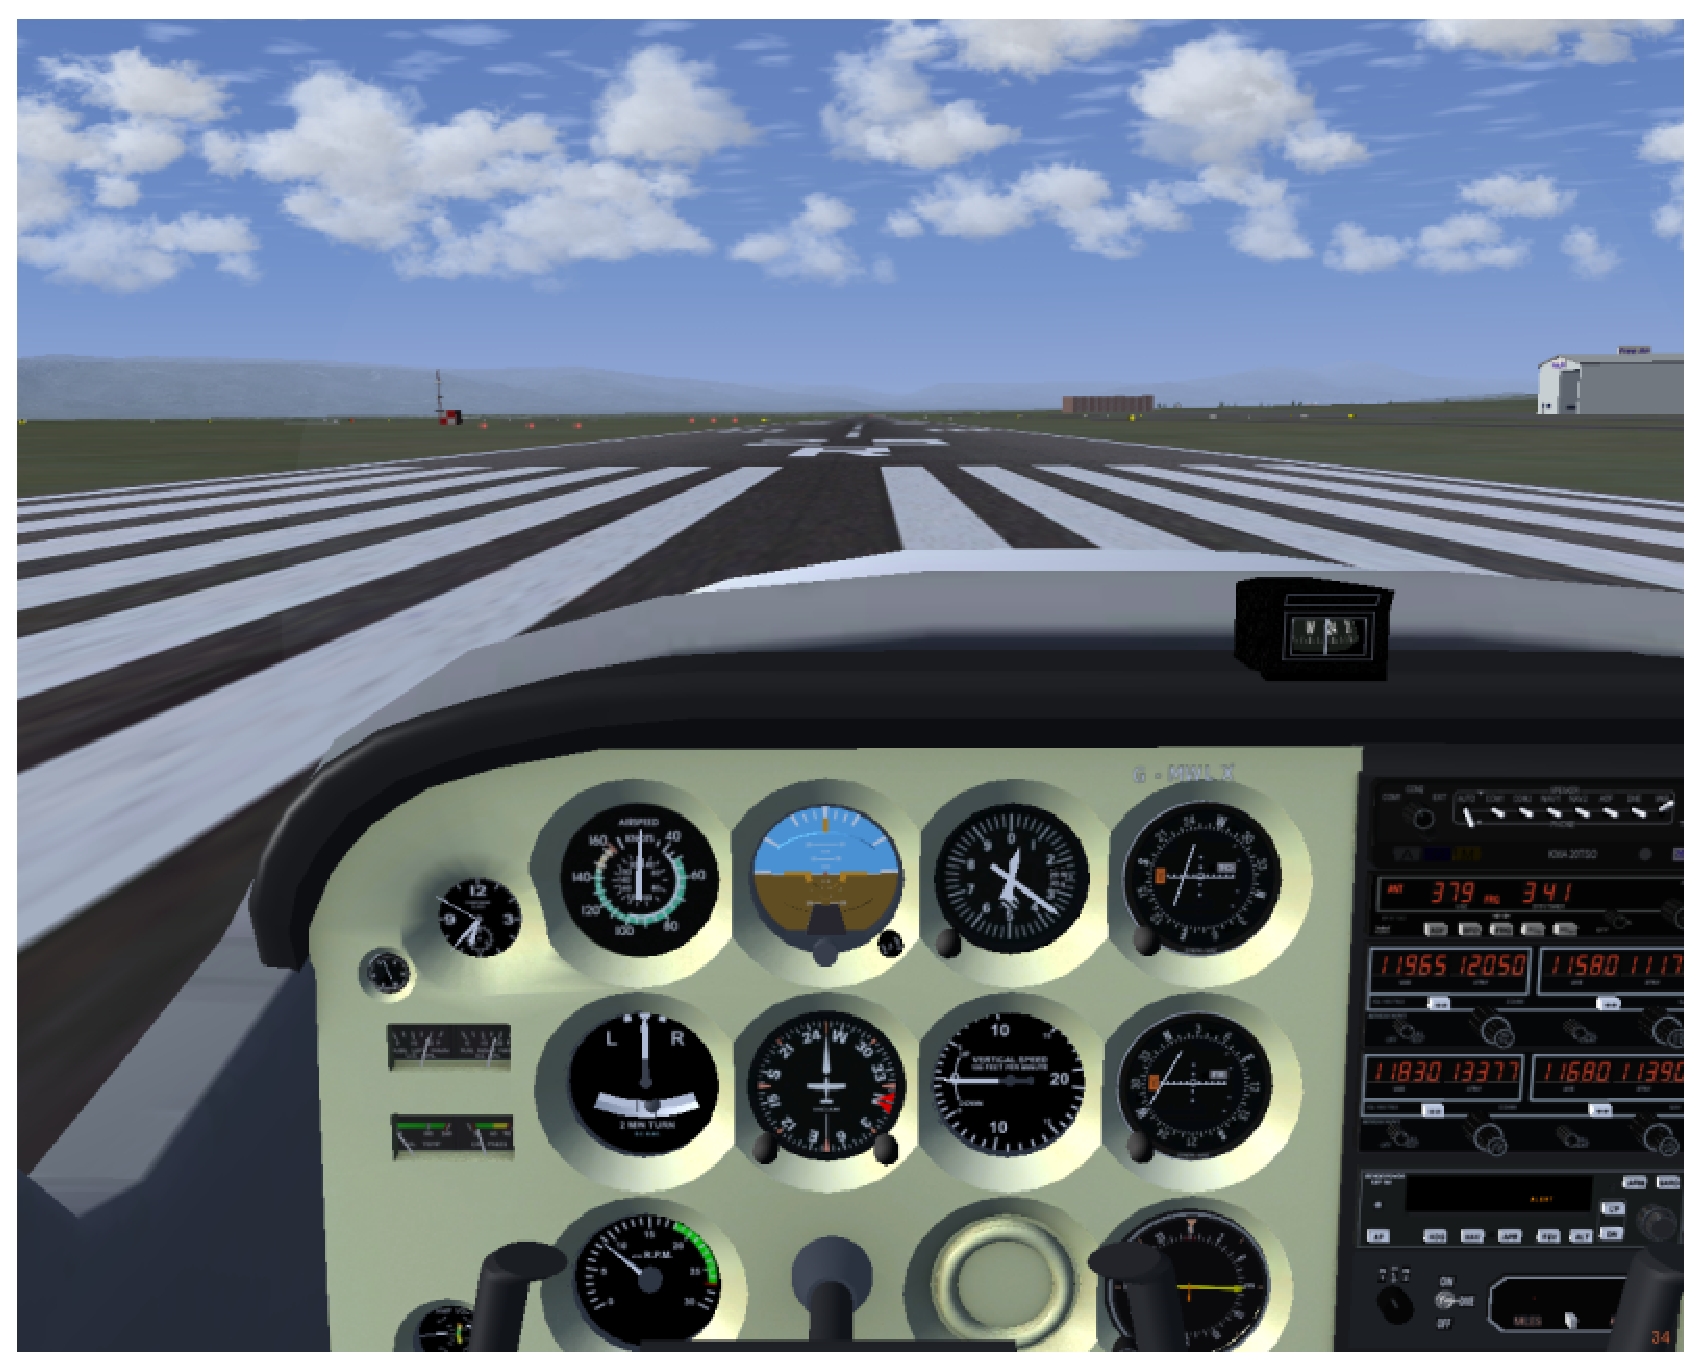
\includegraphics[clip,width=12.5cm]{panel3d}
}}

\smallskip
 \noindent
Fig.\,6: \textit{The 3D cockpit of the Cessna 172.}
\medskip

Aircraft within \FlightGear{} can have both a 2-dimensional instrument panel
and a 3-dimensional cockpit. The 3-dimensional cockpit provides a much
more realistic pilot-eye view, but can be difficult to read with small
monitors.

The default Cessna 172P (c172p) has both a 3-dimensional and 2-dimensional
cockpit. The 3-dimensional cockpit is activated by default when you start
\FlightGear{}, but you can overlay the 2-dimensional instrument panel by
selecting \texttt{View->Toggle 2D Panel} from the menu, or pressing the ``P'' key.

All panel levers and knobs can be operated with the mouse. To change a
control, just click with the left/middle mouse button on the
corresponding knob/lever. For controls that have a range of positions,
using the middle mouse button for larger adjustments. In general, clicking
on the right side of a control will increase the value, while clicking the left side
of the control will decrease the value.

Some instruments (particularly radios) also support use of a mouse scroll-wheel
to change values.

%%%%%%%%%%%%%%%%%%%%%%%%%%%%%%%%%%%%%%%%%%%%%%%%%%%%%%%%%%%%%%%%%%%%%%%%%%%%%%%%
%%%%%%%%%%%%%%%
\section{The Head Up Display\index{head up display}}
%%%%%%%%%%%%%%%%%%%%%%%%%%%%%%%%%%%%%%%%%%%%%%%%%%%%%%%%%%%%%%%%%%%%%%%%%%%%%%%%
%%%%%%%%%%%%%%%

\FlightGear{} also provides a \Index{HUD} (\textbf{H}ead \textbf{U}p
\textbf{D}isplay) \index{head up display}. HUDs are generally found in military
aircraft and some very advanced jets. However, \FlightGear{} also allows you
to use a HUD on many GA aircraft. To activat the HUD, press `h'.

The \Index{HUD} shown in Fig.\,7  displays all main flight parameters of the
plane. In the center you find the \Index{pitch indicator} (in degrees) with the
\Index{aileron indicator} above and the \Index{rudder indicator} below. A
corresponding scale for the elevator\index{elevation indicator} can be found
to the left of the pitch scale along with a pitch trim indicator. On the bottom
there is a simple \Index{turn indicator}.

There are two scales at the extreme left: The inner one displays the \Index{speed}
 (in kts) while the outer one indicates position of the \Index{throttle}.
The two scales on the extreme right display your \Index{height} - the left one
shows the height above ground while the right of it displays hieght above sea-level,
both being displayed in feet.

Besides this, the \Index{HUD} delivers some additions information. On the upper
left you will find date and time, along with your current position, in \Index{latitude}
and \Index{longitude}.

You can change color of the \textbf{HUD} using the ``H'' or ``'h''  key.
Pressing the toggle ``i/I'' minimizes/maximizes the HUD.

\medskip

 \centerline{\fbox{
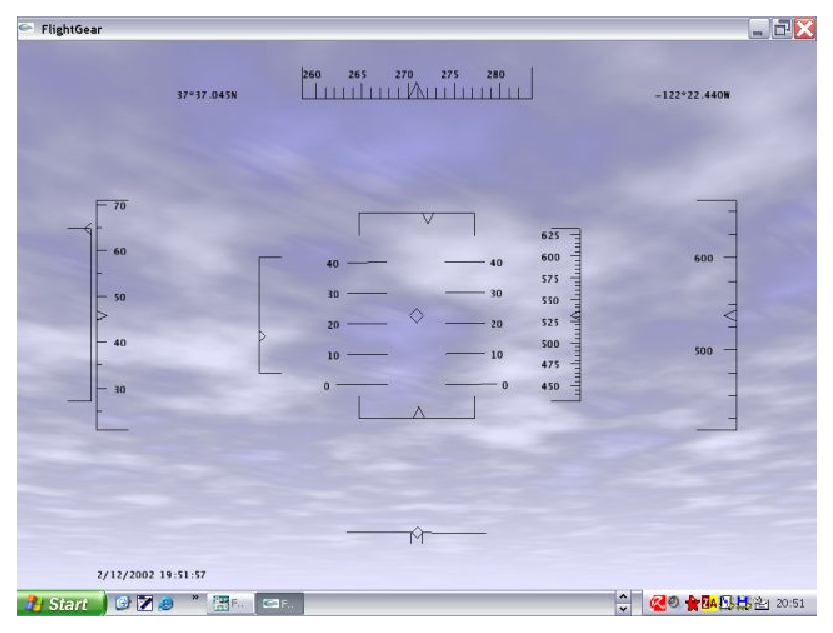
\includegraphics[clip,width=12.5cm]{hud2}
}}

\smallskip
 \noindent
Fig.\,7: \textit{The HUD, or Head Up Display.}
\medskip

%% Revision 0.00  1998/09/08  michael
%% Initial revision for version 0.53.
%% Revision 0.01  1998/09/20  michael
%% several extensions and corrections, added Fig.1.
%% revision 0.10  1998/10/01  michael
%% final proofreading for release
%% revision 0.11  1998/11/01  michael
%% Complete revision of keyborad controls, interesting places
%% revision 0.12  1999/03/07  michael
%% Corrected rudder key
%% revision 0.20  1999/06/04  michael
%% HUD completely rewritten, added panel section with picture, and menu section
%% updated keystrokes
%% revision 0.3 2000/04/20 michael
%% again updated and added keystrokes
%% revised menu entries
%% picture of new panel and re-written panel section
%% added mouse control section
%% Updated many keys, notably autopilot related, added two new tables
%% revision 0.4 2001/05/12 michael
%% updated/added many keystrikes, updated/added panel description
%% (radio stack etc.), new panel pic, panel before HUD now
%% short description of VOR/NDB
%% revision 0.41 2001/01/01 michael
%% added section on flight school material
%% added hints to user configurable *.xml files
%% revision 0.5 2002/01/01 michael
%% revised all changed keybindings now mostly read off of keyboard.xml
%% restructured tables more logically and put into separate files
%% for inclusion in Short Reference
%% New panel picture and revised descirption of panel according to new features
%% New HUD picture
%% revision 0.6 2002/09/05 michael
%% Several corrections/tweaks in plus renumbering of tables
%% Tweaks in menu entries
%% Added 3D cockpit picture
%% Changing numbers in radios
%% Added new menu items, swapped over 3D and 2-D pictures, as 3D cockpit is
%%  now the default
%% Revision 18/10/08: Numerous changes to improve readability, correct spelling errors etc.
%% Revision 8/3/09: Improved description of mouse modes.
%% Revision 26/12/09: Re-organization, move panel description to tutorial, update menu items.


\part{Appendices}
\begin{appendix}
%%
%% getstart.tex -- Flight Gear documentation: The FlightGear Manual
%% Chapter file
%%
%% Written by Michael Basler % Bernhard Buckel, starting September 1998.
%%
%% Copyright (C) 2002 Michael Basler
%%                  & Bernhard Buckel
%%
%% This program is free software; you can redistribute it and/or
%% modify it under the terms of the GNU General Public License as
%% published by the Free Software Foundation; either version 2 of the
%% License, or (at your option) any later version.
%%
%% This program is distributed in the hope that it will be useful, but
%% WITHOUT ANY WARRANTY; without even the implied warranty of
%% MERCHANTABILITY or FITNESS FOR A PARTICULAR PURPOSE.  See the GNU
%% General Public License for more details.
%%
%% You should have received a copy of the GNU General Public License
%% along with this program; if not, write to the Free Software
%% Foundation, Inc., 675 Mass Ave, Cambridge, MA 02139, USA.
%%
%% $Id: missed.tex,v 0.6 2002/09/09 michael
%% (Log is kept at end of this file)

%%%%%%%%%%%%%%%%%%%%%%%%%%%%%%%%%%%%%%%%%%%%%%%%%%%%%%%%%%%%%%%%%%%%%%%%%%%%%%%%%%%%%%%%%%%%%%%
\iflanguage{english}{
\chapter{Missed approach: If anything refuses to work}
}{}
\iflanguage{french}{
\chapter{Approche manqu\'{e}e : si rien ne fonctionne}
}{}
\label{missed}
%%%%%%%%%%%%%%%%%%%%%%%%%%%%%%%%%%%%%%%%%%%%%%%%%%%%%%%%%%%%%%%%%%%%%%%%%%%%%%%%%%%%%%%%%%%%%%%

\iflanguage{english}{
\markboth{\thechapter.\hspace*{1mm} MISSED APPROACH}{\thesection\hspace*{1mm} ???}
}{}
\iflanguage{french}{
\markboth{\thechapter.\hspace*{1mm} APPROCHE MANQUEE}{\thesection\hspace*{1mm} ???}
}{}

\iflanguage{english}{
In the following section, we tried to sort some \Index{problems} according to operating system,
but if you encounter a problem, it may be a wise idea to look beyond ``your'' operating system -- just in case. If you are experiencing problems, we would strongly advise you to first check the \Index{FAQ} maintained by Cameron Moore\index{Moore Cameron} at
}{}
\iflanguage{french}{
Dans la section suivante, nous avons essay\'{e} de trier quelques \Index{probl\`{e}mes} qui peuvent \^{e}tre rencontr\'{e}s, en fonction des syst\`{e}mes d'exploitation. Cependant, si jamais vous rencontrez un probl\`{e}me, sachez qu'il peut parfois \^{e}tre une bonne id\'{e}e de regarder plus loin que ``votre'' syst\`{e}me d'exploitation - au cas o\`{u}. Si vous rencontrez des difficult\'{e}s, nous vous recommandons vivement de consulter en premier lieu la \Index{FAQ} maintenue par Cameron Moore\index{Moore Cameron} \`{a} l'adresse suivante :
}{}

\medskip

\web{http://wiki.flightgear.org/Frequently\_asked\_questions}.
\medskip

\iflanguage{english}{
Moreover, the source code contains a directory \texttt{docs-mini} containing numerous
ideas on and solutions to special problems. This is also a good place to go for further reading.
}{}
\iflanguage{french}{
De plus, le code source comporte un r\'{e}pertoire \texttt{docs-mini} qui contient de nombreuses id\'{e}es
et solutions pour des probl\`{e}mes sp\'{e}cifiques. Il s'agit donc \'{e}galement d'un bon endroit pour trouver d'avantage d'informations.
}{}

%%%%%%%%%%%%%%%%%%%%%%%%%%%%%%%%%%%%%%%%%%%%%%%%%%%%%%%%%%%%%%%%%%%%%%%%%%%%%%%%%%%%%%%%%%%%%%%
\iflanguage{english}{
\section{FlightGear Problem Reports}\index{problem report}
}{}
\iflanguage{french}{
\section{Signaler des probl\`{e}mes relatifs \`{a} FlightGear}\index{signaler un probl\`{e}me}
}{}
%%%%%%%%%%%%%%%%%%%%%%%%%%%%%%%%%%%%%%%%%%%%%%%%%%%%%%%%%%%%%%%%%%%%%%%%%%%%%%%%%%%%%%%%%%%%%%%

\iflanguage{english}{
The best place to look for help is generally the \Index{mailing lists}, specifically the  \textbf{[Flightgear-User]} mailing list. If you happen to be running a Git version of \FlightGear{}, you may want to subscribe to the \textbf{[Flightgear-Devel]} list. Instructions for subscription can be found at
}{}
\iflanguage{french}{
Le meilleur endroit pour obtenir de l'aide est g\'{e}n\'{e}ralement de faire appel aux \Index{listes de diffusion}, et tout particuli\`{e}rement \`{a} la liste de diffusion \textbf{[Flightgear-User]}, ainsi que les \Index{forums}. Si jamais vous utilisez une version Git de \FlightGear{}, vous pourriez vouloir vous inscrire \`{a} la liste de diffusion \textbf{[Flightgear-Devel]}. Les informations pour s'y inscrire peuvent \^{e}tre trouv\'{e}es \`{a} l'adresse :
}{}

 \medskip
\web{http://www.flightgear.org/mail.html}.
 \medskip

\noindent
\iflanguage{english}{
It's often the case that someone has already dealt with the issue you're dealing with, so it may be worth your time to search the mailing list archives at
}{}
\iflanguage{french}{
Bien souvent, vous n'\^{e}tes pas le premier \`{a} rencontrer ce type de difficult\'{e}. Donc une recherche sur les archives des listes de diffusion devrait vous permettre de trouver une solution rapide. Ces archives peuvent \^{e}tre consult\'{e}es \`{a} l'adresse :
}{}

 \medskip

\web{http://sourceforge.net/mailarchive/forum.php?forum\_name=flightgear-users}

\web{http://sourceforge.net/mailarchive/forum.php?forum\_name=flightgear-devel}.
 \medskip

\noindent

\iflanguage{english}{
You should also consider searching the \Index{FlightGear forums} for help, instructions and archives at
}{}
\iflanguage{french}{
Vous devriez \'{e}galement consid\'{e}rer visiter les \Index{forums FlightGear} pour rechercher de l'aide, des instructions et des archives \`{a} l'adresse :
}{}

 \medskip
\web{http://www.flightgear.org/forums}.
 \medskip

\iflanguage{english}{
There are numerous developers and users reading those lists and forums, so questions are generally answered. However, messages of the type
\textit{FlightGear does not compile on my system. What shall I do?}
 \noindent
are hard to answer without any further detail given, aren't they? Here are some things to consider including in your message when you report a problem:
}{}
\iflanguage{french}{
De nombreux d\'{e}veloppeurs et utilisateurs lisent ces listes et forums, donc les questions trouvent g\'{e}n\'{e}ralement une r\'{e}ponse. Cependant, avouez qu'il est difficile de r\'{e}pondre \`{a} des messages du type :
\textit{Je n'arrive pas \`{a} compiler FlightGear sur mon syst\`{e}me, que dois-je faire ?}
 \noindent
si vous ne donnez pas plus de d\'{e}tails, non ? Voici donc quelques \'{e}l\'{e}ments qu'il serait bon d'inclure dans votre message lorsque vous signalez un probl\`{e}me :
}{}

 \medskip

\begin{itemize}
\iflanguage{english}{
\item \textbf{Operating system:} (Linux Fedora 17\ldots/Windows Seven 64 bits\ldots)
\item \textbf{Computer:} (Pentium Dual Core, 2,3GHz\ldots)
\item \textbf{Graphics board/chip:} (ATI Radeon HD 770 XT/NVidia GeForce GTX 590\ldots)
\item \textbf{Compiler/version:} (GCC version 4.6.3\ldots)
\item \textbf{Versions of relevant libraries:} (PLIB 1.8.5, OpenSceneGraph 3.0.1\ldots)
\item \textbf{Type of problem:} (Linker dies with message\ldots)
\item \textbf{Steps to recreate the problem:} Start at KSFO, turn off brakes \ldots
}{}
\iflanguage{french}{
\item \textbf{Syst\`{e}me d'exploitation :} (Linux Fedora 17\ldots/Windows Seven 64 bits\ldots)
\item \textbf{Ordinateur :} (Pentium Dual Core, 2,3 GHz\ldots)
\item \textbf{Carte graphique/processeur :} (ATI Radeon HD 770 XT/Nvidia GeForce GTX 590\ldots)
\item \textbf{Compilateur/version :} (GCC version 4.6.3\ldots)
\item \textbf{Versions des librairies concern\'{e}es :} (PLIB 1.8.5, OpenSceneGraph 3.0.1\ldots)
\item \textbf{Type de probl\`{e}me :} (Le compilateur s'arr\^{e} avec le message suivant\ldots)
\item \textbf{Etapes pour reproduire le probl\`{e}me :} D\'{e}marrer \`{a} KSFO, l\^{a}cher les freins\ldots
}{}
\end{itemize}

\iflanguage{english}{
For getting a trace of the output which \FlightGear{} produces, the following command may come in handy (may need to be modified on some OSs or may not work on others at all, though):
}{}
\iflanguage{french}{
Afin d'obtenir une trace de la sortie que \FlightGear{} produit, la commande suivante peut s'av\'{e}rer utile (elle devra \'{e}ventuellement \^{e}tre adapt\'{e}e sur certains syst\`{e}mes d'exploitation ou peut ne pas fonctionner du tout sur d'autres, d'ailleurs) :
}{}

\medskip

\texttt{\%FG$\underline{~}$ROOT/BIN/fgfs >log.txt 2>\&1}
\medskip

\iflanguage{english}{
\textbf{One final remark:} Please avoid posting binaries to these lists or forums! List subscribers are widely distributed, and some users have low bandwidth and/or metered connections. Large messages may be rejected by the mailing list administrator. Thanks.
}{}
\iflanguage{french}{
\textbf{Une derni\`{e}re petite remarque :} Merci d'essayer d'\'{e}viter de poster du code binaire sur ces forums ou sur ces listes ! Il y a de nombreux abonn\'{e}s et personnes consultant ces informations, et certains disposent de bandes passantes limit\'{e}es et/ou factur\'{e}es. Des messages trop volumineux pourraient \^{e}tre refus\'{e}s par l'administrateur des listes de diffusion. Merci.
}{}

%%%%%%%%%%%%%%%%%%%%%%%%%%%%%%%%%%%%%%%%%%%%%%%%%%%%%%%%%%%%%%%%%%%%%%%%%%%%%%%%%%%%%%%%%%%%%%%
\iflanguage{english}{
\section{General problems}\index{problems!general}
}{}
\iflanguage{french}{
\section{Probl\`{e}mes g\'{e}n\'{e}raux}\index{probl\`{e}mes!g\'{e}n\'{e}raux}
}{}
%%%%%%%%%%%%%%%%%%%%%%%%%%%%%%%%%%%%%%%%%%%%%%%%%%%%%%%%%%%%%%%%%%%%%%%%%%%%%%%%%%%%%%%%%%%%%%%
\begin{itemize}

\iflanguage{english}{
\item{\FlightGear{} runs SOOO slow.}\\
 If \FlightGear{} says it's running with something like 1 fps
 (frame per second) or below you typically don't have working hardware
 \Index{OpenGL} support. There may be several reasons for this. First,
 there may be no OpenGL hardware drivers available for older
 cards. In this case it is highly recommended to get a new board.

 Second, check if your drivers are properly installed. Several
 cards need additional OpenGL support drivers besides the
 ``native'' windows ones.

\item{Either \texttt{configure} or \texttt{make} dies with not found \PLIB{} headers or
 libraries.}\\
  Make sure you have the latest version of \PLIB{} ($>$ version 1.8.4) compiled and installed.
  Its headers like \texttt{pu.h} have to be under \texttt{/usr/include/plib} and its libraries, like \texttt{libplibpu.a} should be under \texttt{/lib}. Double check there are no stray \PLIB{} headers/libraries sitting elsewhere!

  Besides, check carefully the error messages of \texttt{configure}. In several cases, it
  says what is missing.
}{}
\iflanguage{french}{
\item{\FlightGear{} fonctionne siiiiiii lentement.}\\
 Si \FlightGear{} fonctionne, disons \`{a} quelque chose comme une image par seconde
 (\textit{fps, frame per second}), ou moins, c'est que vous n'avez pas de mat\'{e}riel prenant en charge
 \Index{OpenGL}. Il peut y avoir plusieurs raisons \`{a} cela. Tout d'abord, il peut effectivement n'y avoir
 aucun pilote mat\'{e}riel OpenGL disponible pour des cartes anciennes. Dans ce cas, il vous est vivement
 recommand\'{e} d'envisager l'achat d'une nouvelle carte.

 Ensuite, v\'{e}rifiez que vos pilotes sont correctement install\'{e}s. Plusieurs cartes n\'{e}cessites des pilotes
 compl\'{e}mentaires pour faire fonctionner OpenGL en compl\'{e}ment des pilotes ``natifs'' du gestionnaire de fen\^{e}tres.

\item{\texttt{configure} ou \texttt{make} \'{e}chouent car ils ne trouvent pas les en-t\^{e}tes ou biblioth\`{e}ques \PLIB{}.}\\
  Soyez certains de disposer de la derni\`{e}re version de \PLIB{} ($>$ version 1.8.4) compil\'{e}e et install\'{e}e.
  Ses en-t\^{e}tes comme \texttt{pu.h} doivent se situer dans le r\'{e}pertoire \texttt{/usr/include/plib} et ses biblioth\`{e}ques,
  comme\texttt{libplibpu.a}, dans le r\'{e}pertoire \texttt{/lib}. V\'{e}rifiez \`{a} nouveaux qu'il n'y a pas d'autre en-t\^{e}tes ou biblioth\`{e}ques \PLIB{} parasites pr\'{e}sentes ailleurs !

  Enfin, v\'{e}rifiez attentivement les messages d'erreur(s) de \texttt{configure}. Dans de nombreux cas, ils donnent des informations pr\'{e}cieuses sur les \'{e}l\'{e}ments manquants.
}{}

\end{itemize}

%%%%%%%%%%%%%%%%%%%%%%%%%%%%%%%%%%%%%%%%%%%%%%%%%%%%%%%%%%%%%%%%%%%%%%%%%%%%%%%%%%%%%%%%%%%%%%%
\iflanguage{english}{
\section{Potential problems under Linux}\index{problems!Linux}
}{}
\iflanguage{french}{
\section{Probl\`{e}mes potentiels sous Linux}\index{probl\`{e}mes!Linux}
}{}
%%%%%%%%%%%%%%%%%%%%%%%%%%%%%%%%%%%%%%%%%%%%%%%%%%%%%%%%%%%%%%%%%%%%%%%%%%%%%%%%%%%%%%%%%%%%%%%
\iflanguage{english}{
Since we don't have access to all possible flavors of Linux distributions, here are some
thoughts on possible causes of problems. (This Section includes contributions by Kai
Troester.)\index{Troester, Kai}
}{}
\iflanguage{french}{
Comme nous n'avons pas acc\`{e}s \`{a} toutes les versions possibles des distributions Linux, voici quelques-
unes des causes possibles de probl\`{e}mes sous cet environnement. (Cette section comprend des contributions
de Kai Troester.)\index{Troester, Kai}
}{}

\begin{itemize}

\iflanguage{english}{
\item{Wrong library versions}\\
  This is a rather common cause of grief especially when you prefer to
  install the libraries needed by \FlightGear{} by hand. Be sure that
  especially the Mesa library contains support for the
  \Index{3DFX} board and that \Index{GLIDE} libraries are installed and can be
  found. If a \texttt{ldd \`which fgfs\`} complains about missing
  libraries you are in trouble.

  You should also be sure to \emph{always} keep the \emph{latest} version
  of \PLIB{} on your system. Lots of people have
  failed miserably to compile \FlightGear{} just because of an outdated
  plib.
}{}
\iflanguage{french}{
\item{Mauvaises versions des biblioth\`{e}ques}\\
  C'est une origine assez commune de griefs tout sp\'{e}cialement lorsque vous
  pr\'{e}f\'{e}rez installer les biblioth\`{e}ques n\'{e}cessaires \`{a} \FlightGear{}
  \`{a} la main. V\'{e}rifiez bien que, en particulier, la biblioth\`{e}que Mesa comprend bien
  la prise en charge de la carte \Index{3DFX} et que les biblioth\`{e}ques \Index{GLIDE} sont install\'{e}es et qu'elles peuvent \^{e}tre
  trouv\'{e}es. Si un \texttt{ldd \`which fgfs\`} se plaint de biblioth\`{e}ques manquantes, alors vous aurez des difficult\'{e}s.

  Soyez \'{e}galement certain de \emph{toujours} disposer de la \emph{derni\`{e}re} version
  de \PLIB{} sur votre syst\`{e}me. De nombreuses personnes ont lamentablement \'{e}chou\'{e} \`{a} compiler \FlightGear{} simplement
  \`{a} cause d'une version trop ancienne de plib.
}{}

\iflanguage{english}{
\item{Missing \Index{permissions}}\\
 In case you are using \Index{XFree86} before release 4.0 the \FlightGear{} binary may need to be  setuid root in order to be capable of  accessing some accelerator boards (or a special kernel module as described earlier in this document) based on 3DFX chips.
  So you can either issue a

  \texttt{chown root.root /usr/local/bin/fgfs ;}\\
  \texttt{chmod 4755 /usr/local/bin/fgfs}

  to give the \FlightGear{} binary the proper rights or install
  the 3DFX module. The latter is the ``clean''
  solution and strongly recommended!
}{}
\iflanguage{french}{
\item{Droits \Index{manquants}}\\
 Si vous utilisez \Index{XFree86} d'une version ant\'{e}rieure \`{a} 4.0, le binaire \FlightGear{} peut n\'{e}cessiter de disposer du bit setuid
 root afin de pouvoir acc\'{e}der \`{a} certaines cartes d'acc\'{e}l\'{e}ration (ou un module sp\'{e}cial du noyau comme d\'{e}crit pr\'{e}c\'{e}demment dans ce document) bas\'{e}es sur des puces 3DFX.
  Vous pouvez alors essayer un :

  \texttt{chown root.root /usr/local/bin/fgfs ;}\\
  \texttt{chmod 4755 /usr/local/bin/fgfs}

  pour donner au binaire \FlightGear{} les droits appropri\'{e}s ou installer le module 3DFX. Cette derni\`{e}re solution \'{e}tant la plus  ``propre'' et donc fortement recommand\'{e}e !
}{}

\iflanguage{english}{
\item{Non-default install options}\\
  \FlightGear{} will display a lot of diagnostics while starting up.
  If it complains about bad looking or missing files, check that you
  installed them in the way they are supposed to be installed (i.e\. with the latest
  version and in the proper location). The canonical location \FlightGear{}
  wants its data files under \texttt{/usr/local/lib}.
  Be sure to grab the latest versions of everything that might be needed!
}{}
\iflanguage{french}{
\item{Options d'installation particuli\`{e}res}\\
  \FlightGear{} affichera un nombre important d'informations de diagnostic lors de son lancement.
  S'il se plaint de fichiers incorrects ou manquants, v\'{e}rifiez que vous les avez install\'{e}s de
  la mani\`{e}re dont ils sont suppos\'{e}s \^{e}tre install\'{e}s (c'est-\`{a}-dire dans leur version
  la plus r\'{e}cente et \`{a} l'emplacement pr\'{e}vu). L'emplacement canonique de \FlightGear{}
  attend ses donn\'{e}es dans le r\'{e}pertoire \texttt{/usr/local/lib}.
  Soyez certain de r\'{e}cup\'{e}rer les derni\`{e}res versions de tout ce qui peut \^{e}tre n\'{e}cessaire !
}{}

\iflanguage{english}{
\item{Compile problems in general}\\
  Make sure you have the latest (official) version of gcc. Old versions of
  gcc are a frequent source of trouble! On the other hand, some versions
  of the RedHat 7.0 reportedly have certain problems compiling \FlightGear{} as they include
  a preliminary version of gcc.
}{}
\iflanguage{french}{
\item{Probl\`{e}mes plus g\'{e}n\'{e}raux de compilation}\\
  Soyez certain de disposer de la derni\`{e}re version officielle de gcc. D'anciennes version de gcc
  la cause de nombreux probl\`{e}mes ! D'un autre c\^{o}t\'{e}, certaines version de RedHat 7.0 sont connues pour avoir
  des difficult\'{e}s de compilation de \FlightGear{}, car elles incluent une version pr\'{e}liminaire de gcc.
}{}

 \end{itemize}

%%%%%%%%%%%%%%%%%%%%%%%%%%%%%%%%%%%%%%%%%%%%%%%%%%%%%%%%%%%%%%%%%%%%%%%%%%%%%%%%%%%%%%%%%%%%%%%
\iflanguage{english}{
\section{Potential problems under Windows}\index{problems!Windows}
}{}
\iflanguage{french}{
\section{Probl\`{e}mes potentiels sous Windows}\index{probl\`{e}mes!Windows}
}{}
%%%%%%%%%%%%%%%%%%%%%%%%%%%%%%%%%%%%%%%%%%%%%%%%%%%%%%%%%%%%%%%%%%%%%%%%%%%%%%%%%%%%%%%%%%%%%%%
\begin{itemize}
\iflanguage{english}{
\item{The executable refuses to run.}\\
 You may have tried to start the executable directly either by
 double-clicking \texttt{fgfs.exe} in Windows Explorer or by invoking it
 within a MS-DOS shell. Double-clicking via Explorer never works
 (unless you set the environment variable \texttt{FG\_ROOT}
 in \texttt{autoexec.bat} or otherwise). Rather double-click \texttt{fgrun}.
  For more details, check Chapter~\ref{takeoff}.

 Another cause of grief might be that you did not download the
 most recent versions of the base package files required by \FlightGear{}, or
 you did not download any of them at all. Have a close look
 at this, as the scenery/texture format is still under development and may
 change frequently.  For more details, check Chapter~\ref{prefligh}.

 Next, if you run into trouble at runtime, do not use Windows utilities for unpacking the
 \texttt{.tar.gz}. If you did, try it in the Cygnus shell with \texttt{tar xvfz}
 instead.
}{}
\iflanguage{english}{
\item{L'ex\'{e}cutable refuse de se lancer.}\\
 Vous pouvez avoir essay\'{e} de lancer l'ex\'{e}cutable directement en double-cliquant sur \texttt{fgfs.exe}
 dans l'explorateur Windows ou en l'invoquant au travers d'une invite de commandes MS-DOS. Double-cliquer via
 l'explorateur de fonctionne jamais (sauf si vous avez d\'{e}fini la variable d'environnement \texttt{FG\_ROOT}
 dans l'\texttt{autoexec.bat} ou d'une autre mani\`{e}re). Pr\'{e}f\'{e}rez le double-clic sur \texttt{fgrun}.
 Pour plus de d\'{e}tails, consultez le chapitre~\ref{takeoff}.

 Une autre cause de grief peut s'expliquer par le fait que vous n'avez pas t\'{e}l\'{e}charg\'{e} les versions les
 plus r\'{e}centes du paquetage de base n\'{e}cessaires \`{a} \FlightGear{}, ou que vous ne les avez pas t\'{e}l\'{e}charg\'{e}
 du tout. Jetez souvent un \oe{}il \`{a} ceux-ci, car le format des sc\`{e}nes et des textures fait toujours l'objet d'un
 d\'{e}veloppement intensif. Pour plus de d\'{e}tails, reportez-vous au chapitre~\ref{prefligh}.

 Ensuite, si vous rencontrez un probl\`{e}me au d\'{e}marrage, n'utilisez pas les utilitaires Windows pour d\'{e}compresser
 les fichiers \texttt{.tar.gz}. Si vous l'avez fait, essayez de le faire dans l'invite de commandes Cygnus en pr\'{e}f\'{e}rant un \texttt{tar xvfz} \`{a} la place.
}{}

\iflanguage{english}{
\item{\FlightGear{} ignores the command line parameters.}\\
 There can be a problem with passing command line options containing a
 ''='' on the command line. Instead create a batch job to include your options and run that instead.
}{}
\iflanguage{french}{
\item{\FlightGear{} ignore les param\`{e}tres de ligne de commande.}\\
 Il peut y avoir une difficul\'{e} \`{a} passer des options de ligne de commande contenant un caract\`{e}re ''='' sur la ligne de commande. Pr\'{e}f\'{e}rez plut\^{o}t la cr\'{e}ation d'un fichier \textit{batch} pour y inclure vos options et lancez plut\^{o}t celui-ci.
}{}

\iflanguage{english}{
\item{I am unable to build \FlightGear{} under \Index{MSVC}/\Index{MS DevStudio}.}\\
 By default, \FlightGear{} is build with GNU GCC. The Win32 port of GNU GCC is known as
 \Index{Cygwin}. For hints on \textit{Makefiles} required for MSVC or MSC DevStudio have a look into
}{}
\iflanguage{french}{
\item{Je ne parviens pas \`{a} compiler \FlightGear{} avec \Index{MSVC}/\Index{MS DevStudio}.}\\
 Par d\'{e}faut, \FlightGear{} est compil\'{e} avec GNU GCC. Le portage Win32 de GNU GCC est connu sous le nom de
 \Index{Cygwin}. Pour obtenir des astuces sur les fichiers \textit{Makefile} n\'{e}cessaires pour MSVC ou MSC DevStudio veuillez consulter :
}{}

  \medskip

 \web{https://www.gitorious.org/fg/flightgear/trees/next}.
  \medskip

 \noindent
\iflanguage{english}{
In principle, it should be possible to compile \FlightGear{} with the project files provided with the source code.
}{}
\iflanguage{french}{
En princpe, il devrait \^{e}tre possible de compiler \FlightGear{} \`{a} l'aide des fichiers de projet fournis avec le code source.
}{}

\iflanguage{english}{
\item{Compilation of \FlightGear{} dies.}\\
 There may be several reasons for this, including true bugs. However, before trying to do
 anything else or report a problem, make sure you have the latest version of the
 \Cygwin{} compiler. In case of doubt, start
 \texttt{setup.exe} anew and download and install the most recent versions of bundles
 as they possibly may have changed.
}{}
\iflanguage{french}{
\item{La compilation de \FlightGear{} \'{e}choue.}\\
 Il peut y avoir plusieurs raisons \`{a} cela, y compris l'existence de v\'{e}ritables anomalies. Cependant, avant
 de tenter quoi que ce soit ou de signaler un probl\`{e}me, soyez certain de disposer de la derni\`{e}re version du compilateur
 \Cygwin{}. En cas de doute, lancez \`{a} nouveau \texttt{setup.exe} et t\'{e}l\'{e}chargez et installez la version la plus r\'{e}cente
 de l'ensemble, car il est possible que cette version ait chang\'{e}.
}{}

\end{itemize}


%% revision 0.10  1998/10/01  bernhard
%% added win stuff michael
%% final proofreading for release
%% revision 0.11  1998/11/01  michael
%% Remark on mini-OpenGL drivers, new general Section
%% Access violation error under win32 added
%% Command line problem in win32 added
%% revision 0.12  1999/03/07  bernhard
%% Remark on EGCS compiler
%% revision 0.12  1999/03/07  michael
%% Added Contribution by Kai Troester
%% Reworked Win32 Stuff
%% revision 0.20  1999/06/04  michael
%% added hint to FAQ, gfc problem
%% revision 0.22 XXX
%% added hint on install.exe with Cygnus
%% revision 0.3 2000/04/20 michael
%% hint on revised PLIB paths, removed outdated stuff
%% revision 0.3 2000/04/20 michael
%% Deleted some outdated stuff
%% Added Old PLIB problem
%% revision 0.31 2000/05/01 michael
%% Reworked/Added Achnowledgements
%% Added hint on gunzip/tar from Marc Anderson
%% revision 0.4 2001/05/12 michael
%% added some points (RedHat...), deleted some outdated ones
%% complete rewrite and check still to be done ... sometime
%% revision 0.5 2002/01/01 michael
%% removed several outdated issues
%% Added problem linking MetaKit
%% revision 0.601 2002/09/14 michael
%% activated two links

%%
%% getstart.tex -- Flight Gear documentation: The FlightGear Manual
%% Chapter file
%%
%% Written by Michael Basler % Bernhard Buckel, starting September 1998.
%%
%% Copyright (C) 2002 Michael Basler
%%                  & Bernhard Buckel
%%
%% This program is free software; you can redistribute it and/or
%% modify it under the terms of the GNU General Public License as
%% published by the Free Software Foundation; either version 2 of the
%% License, or (at your option) any later version.
%%
%% This program is distributed in the hope that it will be useful, but
%% WITHOUT ANY WARRANTY; without even the implied warranty of
%% MERCHANTABILITY or FITNESS FOR A PARTICULAR PURPOSE.  See the GNU
%% General Public License for more details.
%%
%% You should have received a copy of the GNU General Public License
%% along with this program; if not, write to the Free Software
%% Foundation, Inc., 675 Mass Ave, Cambridge, MA 02139, USA.
%%
%% $Id: opengl.tex,v 0.6 2002/09/09 michael
%% (Log is kept at end of this file)
%%%%%%%%%%%%%%%%%%%%%%%%%%%%%%%%%%%%%%%%%%%%%%%%%%%%%%%%%%%%%%%%%%%%%%%%%%%%%%%%%%%%%%%%%%%%%%%
\chapter{Some words on OpenGL graphics drivers}
\label{opengl}
%%%%%%%%%%%%%%%%%%%%%%%%%%%%%%%%%%%%%%%%%%%%%%%%%%%%%%%%%%%%%%%%%%%%%%%%%%%%%%%%%%%%%%%%%%%%%%%
\markboth{\thechapter.\hspace*{1mm} GETTING THE ENGINE}{\thesection\hspace*{1mm}
INSTALLING DRIVERS}

\FlightGear{}'s graphics engine is based on a \Index{graphics library} called
\Index{OpenGL}. Its primary advantage is its platform independence, i.\,e., programs
written with \Index{OpenGL} support can be compiled and executed on several platforms,
given the proper drivers having been installed in advance. Thus, independent of if you
want to run the binaries only or if you want to compile the program yourself you must
have some sort of \Index{OpenGL} support installed for your \Index{video card}.

A good review  on OpenGL drivers\index{OpenGL drivers} can be found at
\medskip

\web{http://www.flightgear.org/Hardware}.
 \medskip

 \noindent
 Specific information is collected for windows at
  \medskip

\web{http://www.x-plane.com/SYSREQ/v5ibm.html}
 \medskip

 \noindent
 and for Macintosh at
  \medskip

\web{http://www.x-plane.com/SYSREQ/v5mac.html}.
 \medskip

%%Bernhard, 21.02.1999,25.06.1999
 \noindent
An excellent place to look for documentation about Linux and 3D accelerators is the{\it Linux \Index{Quake} HOWTO} at
 \medskip

\web{http://www.linuxquake.com}.
 \medskip

\noindent
 This should be your first aid in case something goes wrong with your Linux 3D setup.

Unfortunately, there are so many graphics boards, chips and drivers out there that we are
unable to provide a complete description for all systems. Given the present market
dominance of NVIDIA combined with the fact that their chips have indeed been proven
powerful for running \FlightGear{}, we will concentrate on NVIDIA
drivers\index{NVIDIA!drivers} in what follows.

%%%%%%%%%%%%%%%%%%%%%%%%%%%%%%%%%%%%%%%%%%%%%%%%%%%%%%%%%%%%%%%%%%%%%%%%%%%%%%%%%%%%%%%%%%%%%%%
\section{NVIDIA chip based cards under \Index{Linux}\label{nvidialinux}}
%%%%%%%%%%%%%%%%%%%%%%%%%%%%%%%%%%%%%%%%%%%%%%%%%%%%%%%%%%%%%%%%%%%%%%%%%%%%%%%%%%%%%%%%%%%%%%%
Recent \Index{Linux} distributions include and install anything needed to run OpenGL
programs under \Index{Linux}. Usually there is no need to install anything else.

If for whatever reason this does not work, you may try to download the most recent
drivers from the NVIDIA site at
 \medskip

\web{http://www.nvidia.com/Products/Drivers.nsf/Linux.html}
 \medskip

 \noindent
At present, this page has drivers for all NVIDIA chips for the following Linux
distributions:\index{NVIDIA!Linux drivers} RedHat 7.1, Redhat 7.0, Redhat 6.2, Redhat
6.1, Mandrake 7.1, Mandrake 7.2, SuSE 7.1, SuSE 7.0 in several formats (.rpm,\ \.tar.gz).
These drivers support OpenGL natively and do not need any additional stuff.

The page named above contains a detailed \texttt{README and Installation Guide} giving a
step-by-step description, making it unnecessary to copy the material here.
Please enshure to replace any OpenGL related libraries with those that are
shipped with the NVIDIA driver - not only user space libraries but also
those in the X server extension modules directory.

%%%%%%%%%%%%%%%%%%%%%%%%%%%%%%%%%%%%%%%%%%%%%%%%%%%%%%%%%%%%%%%%%%%%%%%%%%%%%%%%%%%%%%%%%%%%%%%
\section{NVIDIA chip based cards under \Index{Windows}\label{nvidiawindows}}
%%%%%%%%%%%%%%%%%%%%%%%%%%%%%%%%%%%%%%%%%%%%%%%%%%%%%%%%%%%%%%%%%%%%%%%%%%%%%%%%%%%%%%%%%%%%%%%

Again, you may first try the drivers coming with your graphics card. Usually they should
include \Index{OpenGL} support. If for whatever reason the maker of your board did not
include this feature into the driver, you should install the \Index{Detonator reference
drivers}\index{NVIDIA!Windows drivers} made by \Index{NVIDIA} (which might be a good idea
anyway). These are available in three different versions (Windows 95/98/ME, Windows 2000,
Windows NT) from
 \medskip

  \web{http://www.nvidia.com/products.nsf/htmlmedia/detonator3.html}
  \medskip

\noindent
 Just read carefully the Release notes to be found on that page. Notably do not
forget to uninstall your present driver and install a standard VGA graphics adapter
before switching to the new NVIDIA drivers first.


%%%%%%%%%%%%%%%%%%%%%%%%%%%%%%%%%%%%%%%%%%%%%%%%%%%%%%%%%%%%%%%%%%%%%%%%%%%%%%%%%%%%%%%%%%%%%%%
\section{3DFX chip based cards under \Index{Windows}\label{3dfxwindows}}
%%%%%%%%%%%%%%%%%%%%%%%%%%%%%%%%%%%%%%%%%%%%%%%%%%%%%%%%%%%%%%%%%%%%%%%%%%%%%%%%%%%%%%%%%%%%%%%

With the Glide drivers no longer provided by 3DFX there seems to be little chance to get
it running (except to find older OpenGL drivers somewhere on the net or privately). All
pages which formerly provided official support or instructions for 3DFX are gone now. For
an alternative, you may want to check the next section, though.


%%%%%%%%%%%%%%%%%%%%%%%%%%%%%%%%%%%%%%%%%%%%%%%%%%%%%%%%%%%%%%%%%%%%%%%%%%%%%%%%%%%%%%%%%%%%%%%
\section{An alternative approach for Windows users}
%%%%%%%%%%%%%%%%%%%%%%%%%%%%%%%%%%%%%%%%%%%%%%%%%%%%%%%%%%%%%%%%%%%%%%%%%%%%%%%%%%%%%%%%%%%%%%%

There is now an attempt to build a program which detects the graphics chip on your board
and automatically installs the appropriate OpenGL drivers. This is called \Index{OpenGL
Setup} and is presently in beta stage. It's home page can be found at
\medskip

\web{http://www.glsetup.com/}.
\medskip

We did not try this ourselves, but would suggest it for those completely lost.

%%%%%%%%%%%%%%%%%%%%%%%%%%%%%%%%%%%%%%%%%%%%%%%%%%%%%%%%%%%%%%%%%%%%%%%%%%%%%%%%%%%%%%%%%%%%%%%
\section{3DFX chip based cards under \Index{Linux}\label{3dfxlinux}}
%%%%%%%%%%%%%%%%%%%%%%%%%%%%%%%%%%%%%%%%%%%%%%%%%%%%%%%%%%%%%%%%%%%%%%%%%%%%%%%%%%%%%%%%%%%%%%%

%% MAS, 19.06.2001
Notably, with \Index{3DFX} now having been taken over by \Index{NVIDIA},
manufacturer's support already has disappeared. However with XFree86-4.x
(with x at least being greater than 1) Voodoo3 cards are known to be pretty
usable in 16 bit color mode. Newer cards should work fine as well. If you
are still running a version of Xfree86 3.X and run into problems, consider
an upgrade. The recent distributions by Debian or SuSE have been reported to
work well.

%%%%%%%%%%%%%%%%%%%%%%%%%%%%%%%%%%%%%%%%%%%%%%%%%%%%%%%%%%%%%%%%%%%%%%%%%%%%%%%%%%%%%%%%%%%%%%%
\section{ATI chip based cards under \Index{Linux}\index{ATI}\label{atilinux}}
%%%%%%%%%%%%%%%%%%%%%%%%%%%%%%%%%%%%%%%%%%%%%%%%%%%%%%%%%%%%%%%%%%%%%%%%%%%%%%%%%%%%%%%%%%%%%%%

There is support for \Index{ATI} chips in XFree86-4.1 and greater. Lots of
AGP boards based on the Rage128 chip - from simple Rage128 board to ATI
Xpert2000 - are mostly usable for FlightGear. Since XFree86-4.1 you can use
early Radeon chips - up to Radeon7500 with XFree86-4.2, up to Radeon9100
with XFree86-4.3.
Be careful with stock XFree86-4.3.0, it was released with (known) bugs in
the Radeon driver. Ongoing development provides functional drivers for R100
(Radeon7000 up to 7500) and R200 (Radeon8500 and 9100) chips.

ATI provides an alternative with their binary drivers. You need to build a
kernel module using a script that is supplied with the package and add
several X server modules into your XFree86 tree. In most cases, the RPM
installation will do that for you.

%%%%%%%%%%%%%%%%%%%%%%%%%%%%%%%%%%%%%%%%%%%%%%%%%%%%%%%%%%%%%%%%%%%%%%%%%%%%%%%%%%%%%%%%%%%%%%%
\section{Building your own OpenGL support under \Index{Linux}\index{OpenGL}\label{ownopengl}}
%%%%%%%%%%%%%%%%%%%%%%%%%%%%%%%%%%%%%%%%%%%%%%%%%%%%%%%%%%%%%%%%%%%%%%%%%%%%%%%%%%%%%%%%%%%%%%%

Setting up proper OpenGL support\index{OpenGL!Linux} with a recent Linux
distribution should be pretty simple. As an example \Index{SuSE} ships
everything you need plus some small shell scripts to adjust the missing bits
automagically. If you just want to execute pre-built binaries of FlightGear,
then you're done by using the supplied \FlightGear{} package plus the
mandantory runtime libraries (and kernel modules). The package manager will
tell you which ones to choose.

In case you want to run a self-made kernel, you want to compile
\FlightGear{} yourself, you're tweaking your X server configuration file
yourself or you even run a homebrewed Linux ``distribution'' (this means,
you want to compile everything yourself), this chapter might be useful for
you.

Now let's have a look at the parts that build OpenGL support on Linux. First
there's a Linux kernel with support for your graphics adapter.

Examples on which graphics hardware is supported natively by Open Source
drivers are provided on
\medskip

\noindent
\web{http://dri.sourceforge.net/dri\_status.phtml}.
\medskip

There are a few graphics chip families that are not directly or no more than
partly supported by \Index{XFree86}, the X window implementation on Linux,
because vendors don't like to provide programming information on their
chips. In these cases - notably IBM/DIAMOND/now: \Index{ATI} FireGL graphics
boards and \Index{NVIDIA} GeForce based cards - you depend on the
manufacturers will to follow the ongoing development of the XFree86 graphics
display infrastructure. These boards might prove to deliver impressing
performance but in many cases - considering the CPU's speed you find in
today's PC's - you have many choices which all lead to respectable
performance of \FlightGear{}.

As long as you use a distribution provided kernel, you can expect to find
all necessary kernel modules at the appropriate location. If you compile the
kernel yourself, then you have to take care of two sub-menus in the kernel
configuration menu. You'll find them in the ``Character devices'' menu.
Please notice that AGP support is not compulsory for hardware accelerated
OpenGL support on Linux. This also works quite fine with some PCI cards
(\Index{3dfx} Voodoo3 PCI for example, in case you still own one). Although
every modern PC graphics card utilizes the AGP `bus' for fast data transfer.

Besides ''\Index{AGP Support}'' for your chipset - you might want to ask
your mainboard manual which one is on - you definitely want to activate
``Direct Rendering Manager'' for your graphics board. Please note that
recent releases of XFree86 - namely 4.1.0 and higher might not be supported
by the DRI included in older Linux kernels. Also newer 2.4.x kernels from
2.4.8 up to 2.4.17 do not support DRI in XFree86-4.0.x.

After building and installing your kernel modules and the kernel itself this
task might be completed by loading the `agpgart' module manually or, in case
you linked it into the kernel, by a reboot in purpose to get the new kernel
up and running. While booting your kernel on an AGP capable mainboard you
may expect boot messages like this one:
\medskip

\begin{ttfamily}
\noindent
> Linux agpgart interface v0.99 (c) Jeff Hartmann\\
> gpgart: Maximum main memory to use for agp memory: 439M\\
> agpgart: Detected Via Apollo Pro chipset\\
> agpgart: AGP aperture is 64M @ 0xe4000000
\end{ttfamily}
\medskip

If you don't encounter such messages on Linux kernel boot, then you might
have missed the right chip set. Part one of activation hardware accelerated OpenGL support on your Linux system is now completed.

The second part consists of configuring your \Index{X server} for OpenGL\. This is
not a big deal as it simply consists of to instructions to load the
appropriate modules on startup of the X server.
This is done by editing the configuration file \texttt{/etc/X11/XF86Config}. Today's
Linux distributions are supposed to provide a tool that does this job for
you on your demand. Please make sure there are these two instructions:
\medskip


 \texttt{Load ``glx''}
 
 \texttt{Load ``dri''}
\medskip

\noindent
in the ``Module'' section your \Index{X server} configuration file. If everything is
right the X server will take care of loading the appropriate Linux kernel
module for DRI support of your graphics card. The right Linux kernel module
name is determined by the `Driver' statement in the ``Device'' section of the
XF86Config. Please see three samples on how such a ``Device'' section should
look like:
\medskip

\begin{ttfamily}
\noindent
  Section ``Device''
    
  
    BoardName  	``3dfx Voodoo3 PCI'' 
        
    BusID  	``0:8:0''
        
    Driver  	``tdfx''
    
    Identifier  ``Device[0]''
    
    Screen  	0
    
    VendorName  ``3Dfx''
    
 
\noindent   
  EndSection
  \medskip

\noindent   
  Section ``Device''
  
  
    BoardName  	``ATI Xpert2000 AGP''
    
    BusID  	``1:0:0''
    
    Driver  	``ati''
    
    Option	``AGPMode'' ``1''
    
    Identifier  ``Device[0]''
    
    Screen  	0
    
    VendorName  ``ATI''
    
 \noindent   
  EndSection
 \medskip

\noindent   
  Section ``Device''
  
    BoardName    ``ATI Radeon 32 MB DDR AGP''
    
    BusID        ``1:0:0''
    
    Driver       ``radeon''
    
    Option	 ``AGPMode'' ``4''
    
    Identifier   ``Device[0]''
    
    Screen       0
    
    VendorName   ``ATI''
    
\noindent   
  EndSection
  \medskip
  \end{ttfamily}

By using the Option ``AGPMode'' you can tune AGP performance as long as the
mainboard and the graphics card permit. The BusID on \Index{AGP} systems should
always be set to ``1:0:0'' - because you only have one AGP slot on your board
- whereas the \Index{PCI} BusID differs with the slot your graphics card has been
applied to. `lspci' might be your friend in desperate situations. Also a
look at the end of /var/log/XFree86.0.log, which should be written on X
server startup, should point to the PCI slot where your card resides.

This has been the second part of installing hardware accelerated OpenGL
support on your Linux box.

The third part carries two subparts: First there are the OpenGL runtime
libraries,\index{OpenGL!runtime libraries} sufficient to run existing appliactions. For compiling FlightGear you also need the suiting developmental headers.
As compiling the whole X window system is not subject to this abstract we
expect that your distribution ships the necessary libraries and headers. In
case you told your package manager to install some sort of OpenGL support
you are supposed to find some OpenGL test utilities, at least there should
be `glxinfo' or `gl-info'.

These command-line utilities are useful to say if the previous steps where
successfull. If they refuse to start, then your package manager missed
something because he should have known that these utilities usually depend
on the existence of OpenGL runtime libraries. If they start, then you're one
step ahead. Now watch the output of this tool and and have a look at the
line that starts with

\Index{OpenGL renderer string}:

If you find something like
\medskip

  \texttt{OpenGL renderer string: FireGL2 / FireGL3 (Pentium3)}
  \medskip

\noindent
or
\medskip

  \texttt{OpenGL renderer string: Mesa DRI Voodoo3 20000224}
  \medskip

\noindent
or
\medskip

  \texttt{OpenGL renderer string: Mesa DRI Radeon 20010402}
    
  \texttt{AGP 4x x86}
  \medskip

  \texttt{OpenGL renderer string: Mesa GLX Indirect}
  \medskip

\noindent
mind the word `Indirect', then it's you who missed something, because OpenGL
gets dealt with in a software library running solely on your CPU\. In this
case you might want to have a closer look at the preceding paragraphs of
this chapter. Now please make sure all necessary libraries are at their
proper location.
You will need three OpenGL libraries for running \FlightGear{}. In most cases
you will find them in /usr/lib/:

\texttt{/usr/lib/libGL.so.1}

\texttt{/usr/lib/libGLU.so.1}

\texttt{/usr/lib/libglut.so.3}

These may be the libraries itself or symlinks to appropriate libraries
located in some other directories. Depending on the distribution you use
these libraries might be shipped in different packages. \Index{SuSE} for example
ships libGL in package `xf86\_glx', libGLU in `xf86glu' and libglut in
`mesaglut'. Additionally for \FlightGear{} you need libplib which is part of
the `plib' package.

For compiling \FlightGear{} yourself - as already mentioned - you need the
appropriate header files which often reside in /usr/include/GL/. Two are
necessary for libGL and they come in - no, not `xf86glx-devel' (o.k., they
do but they do not work correctly) but in `mesa-devel':
\medskip

\texttt{/usr/include/GL/gl.h}

\texttt{/usr/include/GL/glx.h}
\medskip

\noindent
One comes with libGLU in `xf86glu-devel':
\medskip

\texttt{/usr/include/GL/glu.h}
\medskip

and one with libglut in `mesaglut-devel'
\medskip

\texttt{/usr/include/GL/glut.h}
\medskip

The `plib' package comes with some more libraries and headers that are too
many to be mentioned here. If all this is present and you have a comfortable
compiler environment, then you are ready to compile \FlightGear{} and enjoy the
result.


Further information on \Index{OpenGL} issues of specific \Index{XFree86} releases is
available here:
\medskip

\underline{http://www.xfree86.org/{$<$}RELEASE NUMBER{$>$}/DRI.html}

\medskip

\noindent
Additional reading on \Index{DRI}:
\medskip

\web{http://www.precisioninsight.com/piinsights.html}
\medskip

\noindent
In case you are missing some `spare parts':
\medskip

\web{http://dri.sourceforge.net/documentation.phtml}


%%%%%%%%%%%%%%%%%%%%%%%%%%%%%%%%%%%%%%%%%%%%%%%%%%%%%%%%%%%%%%%%%%%%%%%%%%%%%%%%%%%%%%%%%%%%%%%
\section{OpenGL on Macintosh}\index{OpenGL!Macintosh}
%%%%%%%%%%%%%%%%%%%%%%%%%%%%%%%%%%%%%%%%%%%%%%%%%%%%%%%%%%%%%%%%%%%%%%%%%%%%%%%%%%%%%%%%%%%%%%%

OpenGL is pre-installed on Mac OS 9.x and later. You may find a newer version than the one installed for \Index{Mac OS 9.x} at
\medskip

\web{http://www.apple.com/opengl}
\medskip

You should receive the updates automatically for \Index{Mac OS X}.


 \noindent
 \textbf{One final word:} We would recommend that you test your \Index{OpenGL} support
 with one of the programs that accompany the drivers, to be absolutely confident
that it is functioning well. There are also many little programs, often available as
screen savers, that can be used for testing.  It is important that you are confident in
your graphics acceleration because \FlightGear{} will try to run the card as fast as
possible. If your drivers aren't working well, or are unstable, you will have difficulty
tracking down the source of any problems and have a frustrating time.

%% Revision 0.00  1998/09/08  michael
%% Initial revision for version 0.53.
%% incl. Linux stuff from b buckel
%% Revision 0.01  1998/09/20  michael
%% several extensions and corrections
%% revision 0.10  1998/10/01  michael
%% added 3dfx stuff from b. buckel
%% final proofreading for release
%% revision 0.11  1998/11/01  michael
%% Remark on mini-OpenGL drivers
%% revision 0.12  1999/03/07  bernhard
%% Complete rewrite of 3DFX/Linux part
%% revision 0.12  1999/03/07  michael
%% Added Riva TNT Win95
%% Added 3DFX Win95
%% revision 0.20  1999/06/04  michael
%% corrections of links
%% revision 0.21 1999/06/30 bernhard
%% updated and expanded 3DFX/Linux
%% revision 0.3 2000/04/20 michael
%% Minor corrections, mainly on software rendering
%% revision 0.31 2000/05/01 michael
%% Added remarks on OpenGL/Matrox by Alex Perry
%% revision 0.5 2002/01/01 michael/martin
%% completely shortened and rewritten
%% removed all stuff old cards, notably 3DFX related
%% added new description for NVIDIA cards
%% removed section on software rendering - no longer useful,
%% added OpenGL setup
%% Section ATI chip based cards under Linux by Martin
%% revision 0.6 2002/01/01 michael
%% removed numerous spelling errors :-(

%%
%% getstart.tex -- Flight Gear documentation: Installation and Getting Started
%% Chapter file
%%
%% Written by Michael Basler, started September 1998.
%%
%% Copyright (C) 2002 Michael Basler
%%
%%
%% This program is free software; you can redistribute it and/or
%% modify it under the terms of the GNU General Public License as
%% published by the Free Software Foundation; either version 2 of the
%% License, or (at your option) any later version.
%%
%% This program is distributed in the hope that it will be useful, but
%% WITHOUT ANY WARRANTY; without even the implied warranty of
%% MERCHANTABILITY or FITNESS FOR A PARTICULAR PURPOSE.  See the GNU
%% General Public License for more details.
%%
%% You should have received a copy of the GNU General Public License
%% along with this program; if not, write to the Free Software
%% Foundation, Inc., 675 Mass Ave, Cambridge, MA 02139, USA.
%%
%% $Id: landing.tex,v 0.6 2002/09/09 michael
%% (Log is kept at end of this file)

%%%%%%%%%%%%%%%%%%%%%%%%%%%%%%%%%%%%%%%%%%%%%%%%%%%%%%%%%%%%%%%%%%%%%%%%%%%%%%%%%%%%%%%%%%%%%%%
\chapter{Landing: Some further thoughts before leaving the plane\label{landing}}
%%%%%%%%%%%%%%%%%%%%%%%%%%%%%%%%%%%%%%%%%%%%%%%%%%%%%%%%%%%%%%%%%%%%%%%%%%%%%%%%%%%%%%%%%%%%%%%
\markboth{\thechapter.\hspace*{1mm}
LANDING}{\thesection\hspace*{1mm} THOSE, WHO DID THE WORK}


%%%%%%%%%%%%%%%%%%%%%%%%%%%%%%%%%%%%%%%%%%%%%%%%%%%%%%%%%%%%%%%%%%%%%%%%%%%%%%%%%%%%%%%%%%%%%%%
\section{A Sketch on the \Index{History} of \FlightGear{}}
%%%%%%%%%%%%%%%%%%%%%%%%%%%%%%%%%%%%%%%%%%%%%%%%%%%%%%%%%%%%%%%%%%%%%%%%%%%%%%%%%%%%%%%%%%%%%%%

History may be a boring subject. However, from time to time there are people asking for the history of \FlightGear{}. As a result, we'll give a short outline.

The \FlightGear{} project goes back to a discussion among a group of net citizens in 1996 resulting in a proposal written by David Murr\index{Murr, David} who, unfortunately, dropped out of the project (as well as the net) later. The original \Index{proposal} is still available
from the \FlightGear{} web site and can be found under
 \medskip

\web{http://www.flightgear.org/proposal-3.0.1}.
 \medskip

\noindent
 Although the names of the people and several of the details have changed over time,
the spirit of that proposal has clearly been retained up to the present time.

Actual coding started in the summer of 1996 and by the end of that year essential
graphics routines were completed. At that time, programming was mainly performed and
coordinated by Eric Korpela\index{Korpela, Eric} from Berkeley University. Early code ran
under \Index{Linux} as well as under \Index{DOS}, \Index{OS/2}, \Index{Windows 95/NT},
and \Index{Sun-OS}. This was found to be quite an ambitious project as it involved, among
other things, writing all the \Index{graphics routines} in a system-independent way
entirely from scratch.

Development slowed and finally stopped in the beginning of 1997 when Eric was completing
his thesis. At this point, the project seemed to be dead and traffic on the mailing list
went down to nearly nothing.

It was Curt Olson\index{Olson, Curt} from the University of Minnesota who re-launched the
project in the middle of 1997. His idea was as simple as it was powerful: Why invent the
wheel a second time? There have been several free flight simulators\index{Flight
simulator!free} available running on \Index{workstation}s under different flavors of
\Index{UNIX}. One of these, \Index{LaRCsim} (developed by Bruce Jackson\index{Jackson,
Bruce} from NASA), seemed to be well suited to the approach. Curt took this one apart and
re-wrote several of the routines such as to make them build as well as run on the
intended target platforms. The key idea in doing so was to exploit a system-independent
graphics platform: \Index{OpenGL}.

In addition, a clever decision on the selection of the basic \Index{scenery}
data was made in the very first version. \FlightGear{} scenery is created
based on satellite data published by the \Index{U.\,S. Geological Survey}.
These terrain data are available from
 \medskip

 \href{http://edc.usgs.gov/geodata/}{http://edc.usgs.gov/geodata/}
 \medskip

\noindent
 for the U.S., and
  \medskip

 \href{http://edcdaac.usgs.gov/gtopo30/gtopo30.html}{http://edcdaac.usgs.gov/gtopo30/gtopo30.html},
  \medskip

\noindent
 resp., for other countries. Those freely accessible scenery data, in
 conjunction with scenery building tools included with
 \FlightGear{}$\!$, are an important feature enabling anyone to
  create his or her own scenery.

This new \FlightGear{} code - still largely being based on the original \Index{LaRCsim}
code - was released in July 1997. From that moment the project gained momentum again.
Here are some milestones in the more recent development history.

%%%%%%%%%%%%%%%%%%%%%%%%%%%%%%%%%% List of Development %%%%%%%%%%%%%%%%%%%%%%%%%%%%%
%%%%%%%%%%%%%%%%%%%%%%%%%Scenery%%%%%%%%%%%%%%%%%%%%%%%%%%%%%%%%%%%%%%
\subsection{Scenery}\index{history!scenery}
\begin{itemize}

\item Texture support\index{textures} was added by Curt
Olson\index{Olson, Curt} in spring 1998. This marked a significant
improvement in terms of reality. Some high-quality \Index{textures} were
submitted by Eric Mitchell\index{Mitchell, Eric} for the \FlightGear{}
project. Another set of high-quality textures was added by Erik
Hofman\index{Hofman, Erik} ever since.

 \item After improving the \Index{scenery} and \Index{texture} support  frame rate\index{frame rate} dropped down to a point where \FlightGear{} became unflyable in spring 1998. This issue was resolved by exploiting hardware \Index{OpenGL}  support, which became available at that time, and implementing  \Index{view frustrum culling} (a rendering technique that ignores the
 part of the scenery not visible in a scene), done by Curt Olson\index{Olson, Curt}.
 With respect to \Index{frame rate} one should keep in mind that the code, at present, is in no way optimized, which leaves room for further improvements.
 \item In September 1998 Curt Olson\index{Olson, Curt}  succeeded in creating a complete terrain model for the U.S. The  scenery is available worldwide now, via a clickable map \index{map, clickable} at:
   \medskip

\web{http://www.flightgear.org/Downloads/world-scenery.html}.
 \medskip

\item Scenery\index{scenery} was further improved by adding \Index{geographic features} including lakes, rivers,and coastlines later, an effort still going on. Textured runways were added by Dave Cornish\index{Cornish, Dave} in spring 2001. Light textures\index{light textures} add to the visual impression at night. To cope with the constant growth of scenery data, a binary scenery format was introduced in spring 2001. Runway lighting\index{runway lighting} was introduced by Curt Olson\index{Olson, Curt} in spring 2001. Finally, a completely new set of \Index{scenery} files for the whole world was created by William Riley\index{Riley, William} based on preparatory documentation by David Megginson\index{Megginson, David} in summer 2002. This is based on a data set called VMap0\index{VMap0 data} as an alternative to the \Index{GSHHS data} used so far. This scenery is a big improvement as it has world wide coverage of main streets, rivers, etc., while it's downside are much less accurate coast lines. \FlightGear{}'s base scenery is based on these new scenery files since summer 2002. The complete set is available via a clickable map,\index{map, clickable} too, from
\medskip

\web{http://www.randdtechnologies.com/fgfs/newScenery/world-scenery.html}.
 \medskip
 \item There was support added for \Index{static objects} to the scenery in 2001, which permits placing buildings, static planes, trees and so on in the scenery. However, despite a few proofs of concept systematic inclusion of these landmarks is still missing.
\item The world is populated with \Index{random ground objects} with appropriate type and density for the local ground cover type since summer 2002. This marks a mayor improvement of reality and is mainly thanks to work by D. Megginson\index{Megginson, David}.
\end{itemize}

%%%%%%%%%%%%%%%%%%%%%%%%%Aircraft%%%%%%%%%%%%%%%%%%%%%%%%%%%%%%%%%%%%%%
\subsection{Aircraft}\index{history!aircraft}
\begin{itemize}
\item A \Index{HUD} (\Index{head up display}) was added based on code
 provided by Michele America\index{America, Michele} and Charlie Hotch\-kiss\index{Hotchkiss, Charlie} in the fall of 1997 and was improved later by Norman Vine. While not generally available for real \Index{Cessna 172}, the HUD conveniently reports the actual flight performance of the simulation and may be of further use in military jets later.
 \item A rudimentary \Index{autopilot} implementing heading hold was
contributed by Jeff Goeke-Smith\index{Goeke-Smith, Jeff} in April 1998. It was improved
by the addition of an altitude hold and a terrain following switch in October 1998 and
further developed by Norman Vine\index{Vine, Norman} later.
\item Friedemann Reinhard \index{Reinhard, Friedemann} developed early \Index{instrument panel} code, which was added in June 1998. Unfortunately, development of that panel slowed down later. Finally, David Megginson \index{Megginson, David} decided to rebuild the panel code from scratch in January 2000. This led to a rapid addition of new instruments and features to the panel, resulting in nearly all main instruments being included until spring 2001. A handy minipanel was added in summer 2001.
\item Finally, \Index{LaRCsim}s \Index{Navion} was replaced as the default aircraft
 when the \Index{Cessna 172} was stable enough in February 2000 - as move most users will welcome. There are now several \Index{flight model} and airplane options to choose from at runtime. Jon Berndt\index{Berndt, Jon, S.} has invested a lot of time in a more
realistic and versatile flight model with a more powerful aircraft configuration method.
\JSBSim, as it has come to be called, did replace LaRCsim as the default
\Index{flight dynamics model} (\Index{FDM}), and it is planned to include such features as fuel slosh effects, turbulence, complete flight control systems, and other features not often found
all together in a flight simulator. As an alternative, Andy Ross\index{Ross, Andy} added another flight dynamics model called \YASim{} (Yet Another Flight Dynamics Simulator) which aims at simplicity of use and is based on fluid dynamics, by the end of 2001. This one bought us flight models for a 747, an A4, and a DC-3. Alternatively, a group around Michael Selig\index{Selig, Michael} from the \Index{UIUC} group provided another flight model along with several planes since around 2000.
\item A fully operational \Index{radio stack} and working radios were added to the panel by Curt Olson\index{Olson, Curt} in spring 2000. A huge database of Navaids contributed by Robin
Peel\index{Peel, Robin} allows IFR navigation since then. There was basic \Index{ATC} support added in fall 2001 by David Luff\index{Luff, David}. This is not yet fully implemented, but displaying \Index{ATIS messages} is already possible. A \Index{magneto switch} with proper functions was added at the end of 2001 by John Check\index{Check, John} and David Megginson.\index{Megginson, David}. Moreover, several panels were continually improved during 2001 and 2002 by John and others. \FlightGear{} now allows flying ILS approaches and features a \Index{Bendix transponder}.
\item In 2002 functional \Index{multi-engine support} found it's way into
\FlightGear{}. \JSBSim{} is now the default FDM in \FlightGear{}.
\item Support of ''true'' \Index{3D panels} became stable via contributions from John Check\index{Check, John} and others in spring 2002. In addition, we got movable control surfaces\index{control surface, movable} like propellers etc., thanks to David Megginson.\index{Megginson, David}
\end{itemize}

%%%%%%%%%%%%%%%%%%%%%%%%%Environment%%%%%%%%%%%%%%%%%%%%%%%%%%%%%%%%%%%%%%
\subsection{Environment}\index{history!environment}
\begin{itemize}
\item The display of sun, moon and stars have been a weak point for PC flight simulators
 for a long time. It is one of the great achievements of \FlightGear{} to include accurate modeling and display of sun, moon, and planets very early. The corresponding \Index{astronomy code} was implemented in fall 1997 by Durk Talsma\index{Talsma, Durk}.
\item Christian Mayer, \index{Mayer, Christian}  together with Durk Talsma,\index{Talsma, Durk}
contributed weather code in the winter of 1999. This included \Index{clouds}, \Index{winds}, and even \Index{thunderstorms}.
\end{itemize}

%%%%%%%%%%%%%%%%%%%%%%%%%User Interface%%%%%%%%%%%%%%%%%%%%%%%%%%%%%%%%%%%%%%
\subsection{User Interface}\index{history!user interface}
\begin{itemize}
\item The foundation for a menu system\index{menu} was laid based on another library,
 the Portable Library \PLIB\index{PLIB}, in June 1998. After having been idle for a time, the first working menu entries came to life in spring 1999.
 
  \PLIB{} underwent rapid development later. It has been distributed as a separate package by
  Steve Baker\index{Baker, Steve} with a much broader range of applications in mind, since spring 1999. It  has provided the basic graphics rendering engine for \FlightGear{} since fall 1999. 
\item In 1998 there was basic \Index{audio support}, i.\,e. an audio library
and some basic background engine sound. This was later integrated into the
above-mentioned portable library, \PLIB\index{PLIB}. This same library was extended to
support joystick/yoke/rudder\index{joystick} in October 1999, again marking a huge step
in terms of realism. To adapt on different joystick, configuration options were
introduced in fall 2000. Joystick support was further improved by adding a self detection\index{joystick/self detection} feature based on xml joystick files, by David Megginson\index{Megginson, David} in summer 2002.
\item Networking/multiplayer\index{networking code}\index{multiplayer code}
 code has been integrated by Oliver Delise \index{Delise, Oliver} and Curt
Olson\index{Olson, Curt} starting fall 1999. This effort is aimed at enabling
\FlightGear{}  to run concurrently on several machines over a \Index{network}, either an Intranet or the \Index{Internet}, coupling it to a \Index{flight planner} running on a second
machine, and more. There emerged several approaches for remotely controlling \FlightGear{} over a Network during 2001. Notably there was added support for the ''Atlas''\index{Atlas} moving map program. Besides, an embedded \Index{HTTP server} developed by Curt Olson\index{Olson, Curt} late in 2001 can now act a \Index{property manager} for external programs.
\item Manually changing \Index{views} in a flight simulator is in a sense always ''unreal'' but
nonetheless required in certain situations. A possible solution was supplied by Norman
Vine\index{Vine, Norman} in the winter of 1999 by implementing code for changing views
using the mouse. Alternatively, you can use a hat switch for this purpose, today.
\item A \Index{property manager} was implemented by David Megginson\index{Megginson, David} in
fall 2000. It allows parsing a file called \texttt{.fgfsrc}\index{.fgfsrc} under
UNIX/Linux and \texttt{system.fgfsrc}\index{system.fgfsrc} under Windows for input
options. This plain ASCII file has proven useful in submitting the growing number of
input options, and notably the \Index{joystick settings}. This has shown to be a useful
concept, and joystick, keyboard, and panel settings are no longer hard coded but set
using *.xml files since spring 2001 thanks to work mainly by David Megginson and John
Check.\index{Check, John}
\end{itemize}
%%%%%%%%%%%%%%%%%%%%%%%%%%%%%%%%%% End List of Development %%%%%%%%%%%%%%%%%%%%%%%%%

During development there were several code reorganization efforts. Various code
subsystems were moved into packages. As a result, code is organized as follows at present:
\medskip

The base of the graphics engine is \textbf{\Index{OpenGL}}, a platform independent
graphics library. Based on \Index{OpenGL}, the Portable Library \PLIB{}\index{PLIB}
provides basic rendering, audio, joystick etc. routines. Based on \PLIB\index{PLIB} is
\SimGear{}\index{SimGear}, which includes all of the basic routines required for the
flight simulator as well as for building scenery. On top of \SimGear{}\index{SimGear}
there are (i) \FlightGear{}\index{FlightGear} (the simulator itself), and (ii)
\TerraGear{}\index{TerraGear}, which comprises the scenery building tools.

This is by no means an exhaustive history and most likely some people who have made
important contributions have been left out. Besides the above-named contributions there
was a lot of work done concerning the internal structure by: Jon S. Berndt\index{Berndt,
Jon, S.}, Oliver Delise, \index{Delise, Oliver} Christian Mayer, \index{Mayer, Christian}
Curt Olson,\index{Olson, Curt} Tony Peden, \index{Peden, Tony} Gary R. Van
Sickle\index{van Sickle, Gary, R.}, Norman Vine\index{Vine, Norman}, and others. A more
comprehensive list of contributors can be found in Chapter \ref{landing} as well as in
the \texttt{Thanks} file provided with the code. Also, the \FlightGear{}
Website\index{FlightGear Website} contains a detailed history worth reading of all of the
notable development milestones at
 \medskip

 \web{http://www.flightgear.org/News/}

%%%%%%%%%%%%%%%%%%%%%%%%%%%%%%%%%%%%%%%%%%%%%%%%%%%%%%%%%%%%%%%%%%%%%%%%%%%%%%%%%%%%%%%%%%%%%%%
\section{Those, who did the work}\index{contributors}
%%%%%%%%%%%%%%%%%%%%%%%%%%%%%%%%%%%%%%%%%%%%%%%%%%%%%%%%%%%%%%%%%%%%%%%%%%%%%%%%%%%%%%%%%%%%%%%

Did you enjoy the flight? In case you did, don't forget those who devoted hundreds of
hours to that project. All of this work is done on a voluntary basis within spare time,
thus bare with the \Index{programmers} in case something does not work the way you want
it to. Instead, sit down and write them a kind (!) mail proposing what to change.
Alternatively, you can subscribe to the \FlightGear{} \Index{mailing lists} and
contribute your thoughts there. Instructions to do so can be found at
 \medskip

 \web{http://www.flightgear.org/mail.html}.
  \medskip

\noindent
 Essentially there are two lists, one of which being mainly for the developers
and the other one for end users. Besides, there is a very low-traffic list for
announcements.
\medskip

 \noindent
The following names the people who did the job (this information was essentially taken
from the file \texttt{Thanks} accompanying the code).
 \medskip

\noindent \textbf{A1 Free Sounds}\index{A1 Free Sounds} (\mail{techie@mail.ev1.net})\\
   Granted permission for the \FlightGear{} project to use some of the sound effects from their  
   site. Homepage under   
   \medskip
   
   \href{http://www.a1freesoundeffects.com/}{http://www.a1freesoundeffects.com/}
   \medskip

\noindent \textbf{Raul Alonzo}\index{Alonzo, Raul} (\mail{amil@las.es})\\
   Mr. Alonzo is the
 author of Ssystem and provided his kind permission for using the moon texture.
 Parts of his code were used as a template when adding the texture.
  Ssystem Homepage can be found at:
   \medskip

  \href{http://www1.las.es/~amil/ssystem/}{http://www1.las.es/$\tilde{~~}$amil/ssystem/}.
 \medskip

 \noindent \textbf{Michele America}\index{America, Michele}
(\mail{nomimarketing@mail.telepac.pt})\\
  Contributed to the \Index{HUD} code.
 \medskip

\noindent \textbf{Michael Basler}\index{Basler, Michael} (\mail{pmb@epost.de})\\
 Author of Installation and Getting Started. Flight Simulation Page at
  \medskip

 \web{http://www.geocities.com/pmb.geo/flusi.htm}
\medskip

\noindent \textbf{Jon S. Berndt}\index{Berndt, Jon, S.} (\mail{jsb@hal-pc.org})\\
 Working on a complete C++ rewrite/reimplimentation of the core \Index{FDM}.
  Initially he is using X15 data to test his code, but once things are
  all in place we should be able to simulate arbitrary aircraft. Jon
  maintains a page dealing with Flight Dynamics at:
   \medskip

  \href{http://jsbsim.sourceforge.net/}{http://jsbsim.sourceforge.net/}
   \medskip

\noindent
  Special attention to X15 is paid in separate pages on this site. Besides, Jon
  contributed via a lot of suggestions/corrections to this Guide.
\medskip

\noindent \textbf{Paul Bleisch}\index{Bleisch, Paul} (\mail{pbleisch@acm.org})\\
  Redid the debug system so that it would be much more
  flexible, so it could be easily disabled for production system, and
  so that messages for certain subsystems could be selectively
  enabled. Also contributed a first stab at a config file/command line parsing
  system.
 \medskip


\noindent \textbf{Jim Brennan}\index{Brennan, Jim} (\mail{jjb@kingmont.com})\\
  Provided a big chunk of online space to store USA scenery for \FlightGear{}$\!$.
 \medskip

\noindent \textbf{Bernie Bright}\index{Bright, Bernie}
(\mail{bbright@bigpond.net.au})\\
  Many C++ style, usage, and implementation improvements, STL
  portability and much, much more.
  Added threading support and a threaded tile pager.
 \medskip

\noindent \textbf{Bernhard H. Buckel}\index{Buckel, Bernhard}
(\mail{buckel@mail.uni-wuerzburg.de})\\
  Contributed the README.Linux.  Contributed several sections to earlier versions of
 Installation and Getting Started.
 \medskip

\noindent \textbf{Gene Buckle}\index{Buckle, Gene} (\mail{geneb@deltasoft.com})\\
  A lot of work getting \FlightGear{} to compile with the \Index{MSVC}++
  compiler. Numerous hints on detailed improvements.
 \medskip


\noindent \textbf{Ralph Carmichael}\index{Carmichael, Ralph} (\mail{ralph@pdas.com})\\
  Support of the project. The Public Domain Aeronautical Software web site at
\medskip

\href{http://www.pdas.com/}{http://www.pdas.com/}
 \medskip

 \noindent
 has the PDAS CD-ROM for sale containing great programs for astronautical engineers.

\noindent \textbf{Didier Chauveau}\index{Chauveau, Didier}
(\mail{chauveau@math.univ-mlv.fr})\\
  Provided some initial code to parse the 30 arcsec DEM files found at:
   \medskip

  \href{http://edcwww.cr.usgs.gov/landdaac/gtopo30/gtopo30.html}{http://edcwww.cr.usgs.gov/landdaac/gtopo30/gtopo30.html}.
 \medskip

\noindent \textbf{John Check}\index{Check, John} (\mail{j4strngs@rockfish.net})\\
 John maintains the base package CVS repository. He contributed cloud textures, wrote an excellent Joystick Howto as well as a panel Howto. Moreover, he contributed new instrument panel configurations. \FlightGear{}
 page at
 \medskip

 \href{http://www.rockfish.net/fg/}{http://www.rockfish.net/fg/}.
 \medskip

\noindent \textbf{Dave Cornish}\index{Cornish, Dave} (\mail{dmc@halcyon.com})\\
 Dave created new cool runway textures plus some of our cloud textures.
 \medskip

\noindent \textbf{Oliver Delise} \index{Delise, Oliver} (\mail{delise@mail.isis.de})\\
 Started a FAQ, Documentation, Public relations. Working on adding some
  networking/multi-user code.\index{networking code} Founder of the FlightGear MultiPilot
  Project at
   \medskip

  \href{http://www.isis.de/members/~odelise/progs/flightgear/}{http://www.isis.de/members/$\tilde{~~}$odelise/progs/flightgear/}.
\medskip

\noindent \textbf{Jean-Francois Doue}\index{Doue, Jean-Francois}\\
  Vector 2D, 3D, 4D and Matrix 3D and 4D inlined C++ classes.  (Based on
  Graphics Gems IV, Ed. Paul S. Heckbert)
  \medskip

\href{http://www.animats.com/simpleppp/ftp/public_html/topics/developers.html}{http://www.animats.com/simpleppp/ftp/public\_html/topics/developers.html}.
 \medskip

\noindent \textbf{Dave Eberly} \index{Eberly, Dave} (\mail{eberly@magic-software.com})\\
  Contributed some sphere interpolation code used by Christian Mayer's
  weather data base system.  On Dave's web site there are tons of
  really useful looking code at
  \medskip

\href{http://www.magic-software.com/}{http://www.magic-software.com/}.
  \medskip

\noindent \textbf{Francine Evans}\index{Evans, Francine} (\mail{evans@cs.sunysb.edu})
  Wrote the GPL'd tri-striper we use.
  \medskip

\href{http://www.cs.sunysb.edu/~stripe/}{http://www.cs.sunysb.edu/$\tilde{~~}$stripe/}
\medskip

\noindent \textbf{Oscar Everitt}\index{Everitt, Oscar} (\mail{bigoc@premier.net})\\
  Created single engine piston engine sounds as part of an F4U package
  for \Index{FS98}.  They are pretty cool and Oscar was happy to contribute
  them to our little project.
 \medskip

\noindent \textbf{Bruce Finney}\index{Finney, Bruce} (\mail{bfinney@gte.net})\\
  Contributed patches for MSVC5 compatibility.
 \medskip

\noindent \textbf{Melchior Franz}\index{Franz, Melchior} (\mail{a8603365@unet.univie.ac.at})\\
  Contributed joystick hat support, a LED font, improvements of the telnet and the http interface. Notable effort in hunting memory leaks in \FlightGear{}, \SimGear{}, and \JSBSim{}.
  \medskip

\noindent \textbf{Jean-loup Gailly}\index{Gailly, Jean-loup} and \textbf{Mark
Adler}\index{Adler, Mark} (\mail{zlib@gzip.org})\\
  Authors of the \Index{zlib library}.  Used for on-the-fly compression and
  decompression routines,

  \href{http://www.gzip.org/zlib/}{http://www.gzip.org/zlib/}.
 \medskip

\noindent \textbf{Mohit Garg}\index{Garg, Mohit}
(\href{mailto:theprotean_1@hotmail.com}{theprotean\_1@hotmail.com})\\
 Contributed to the manual.
 \medskip

\noindent \textbf{Thomas Gellekum}\index{Gellekum, Thomas}
(\mail{tg@ihf.rwth-aachen.de})\\
  Changes and updates for compiling on \Index{FreeBSD}.
 \medskip

\noindent \textbf{Neetha Girish}\index{Girish, Neetha}
(\mail{neethagirish@usa.net})\\
  Contributed the changes for the xml configurable HUD.
 \medskip

\noindent \textbf{Jeff Goeke-Smith}\index{Goeke-Smith, Jeff}
(\mail{jgoeke@voyager.net})\\
  Contributed our first \Index{autopilot} (Heading Hold).
  Better autoconf check for external timezone/daylight variables.
 \medskip

\noindent \textbf{Michael I. Gold}\index{Gold, Michael, I.}
(\mail{gold@puck.asd.sgi.com})\\
 Patiently answered questions on \Index{OpenGL}.
 \medskip

\noindent \textbf{Habibe}\index{Habibe} (\mail{habibie@MailandNews.com})\\
 Made RedHat package building changes for SimGear.
 \medskip

\noindent \textbf{Mike Hill}\index{Hill, Mike} (\mail{mikehill@flightsim.com})\\
 For allowing us to concert and use his wonderful planes, available form
 \medskip

 \web{http://www.flightsimnetwork.com/mikehill/home.htm},

 \noindent
 for \FlightGear{}.
 \medskip

\noindent \textbf{Erik Hofman}\index{Hofman, Erik} (\mail{erik@ehofman.com})\\
  Major overhaul and parameterization of the sound module to allow
  aircraft-specific sound configuration at runtime.
  Contributed SGI IRIX support (including binaries) and some really great
  textures.
 \medskip

\noindent \textbf{Charlie Hotchkiss}\index{Hotchkiss, Charlie}
(\mail{clhotch@pacbell.net})\\ Worked on improving and enhancing the \Index{HUD} code.
Lots of code style tips and code tweaks.
 \medskip

\noindent \textbf{Bruce Jackson}\index{Jackson, Bruce} (NASA)
(\mail{e.b.jackson@larc.nasa.gov})
 \medskip

   Developed the \Index{LaRCsim} code under funding by NASA which we use to provide the
   flight model. Bruce has patiently answered many, many questions.
 \medskip

  \href{http://dcb.larc.nasa.gov/www/DCBStaff/ebj/ebj.html}{http://dcb.larc.nasa.gov/www/DCBStaff/ebj/ebj.html}
  \medskip


\noindent \textbf{Ove Kaaven} \index{Kaaven, Ove} (\mail{ovek@arcticnet.no})\\
 Contributed the Debian binary.
 \medskip

\noindent \textbf{Richard Kaszeta} \index{Kaszeta, Richard} (\mail{bofh@me.umn.edu})\\
  Contributed screen buffer to ppm screen shot routine.
  Also helped in the early development of the "altitude
  hold autopilot module"\index{autopilot} by teaching Curt Olson the basics of Control Theory
  and helping him code and debug early versions. Curt's ''Boss'' Bob Hain
 (\mail{bob@me.umn.edu}) also contributed to that.  Further details available at:
 \medskip

  \href{http://www.menet.umn.edu/~curt/fgfs/Docs/Autopilot/AltitudeHold/AltitudeHold.html}{http://www.menet.umn.edu/$\tilde{~~}$curt/fgfs/Docs/Autopilot/AltitudeHold/AltitudeHold.html}.
  \medskip

\noindent
  Rich's Homepage is at
  \medskip

  \href{http://www.kaszeta.org/rich/}{http://www.kaszeta.org/rich/}.
  \medskip

\noindent \textbf{Tom Knienieder}\index{Knienieder, Tom} (\mail{tom@knienieder.com})\\
  Ported the audio library\index{audio library} first to OpenBSD and IRIX and after that to Win32.
 \medskip

\noindent \textbf{Reto Koradi}\index{Koradi, Reto} (\mail{kor@mol.biol.ethz.ch})
 \medskip

  Helped with setting up \Index{fog effects}.
 \medskip

\href{http://www.mol.biol.ethz.ch/wuthrich/people/kor/}{http://www.mol.biol.ethz.ch/wuthrich/people/kor/}
 \medskip

\noindent \textbf{Bob Kuehne}\index{Kuehne, Bob} (\mail{rpk@who.net})\\
  Redid the Makefile system so it is simpler and more robust.
 \medskip

\noindent \textbf{Kyler B Laird}\index{Laird, Kyler B.} (\mail{laird@ecn.purdue.edu})\\
 Contributed corrections to the manual.
 \medskip

\noindent \textbf{David Luff}\index{Luff, David} (\mail{david.luff@nottingham.ac.uk})\\
 Contributed heavily to the IO360 piston engine model.
 \medskip

\noindent \textbf{Christian Mayer}\index{Mayer, Christian}
(\mail{flightgear@christianmayer.de})\\
 Working on \Index{multi-lingual conversion tools} for fgfs as a demonstration of technology.
 Contributed code to read Microsoft Flight Simulator scenery textures. Christian is working on a completely new \Index{weather} subsystem.
 Donated a \Index{hot air balloon} to the project.
 \medskip

\noindent \textbf{David Megginson}\index{Megginson, David} (\mail{david@megginson.com})\\
  Contributed patches to allow mouse input to control view direction yoke.
  Contributed financially towards hard drive space for use by the
  flight gear project. Updates to README.running.
  Working on getting fgfs and ssg to work without textures.
  Also added the new 2-D panel and the save/load support.
  Further, he developed new \Index{panel} code, playing better with OpenGL, with new features.
  Developed the property manager and contributed to joystick support.
  Random ground cover objects
 \medskip

 \medskip

\noindent \textbf{Cameron Moore}\index{Moore, Cameron}
(\mail{cameron@unbeatenpath.net})\\
 FAQ maintainer. Reigning list administrator. Provided man pages.
 \medskip

\noindent \textbf{Eric Mitchell}\index{Mitchell, Eric} (\mail{mitchell@mars.ark.com})\\
  Contributed some topnotch scenery \Index{textures} being all original creations by him.
 \medskip

\noindent \textbf{Anders Morken}\index{Morken, Anders} (\mail{amrken@online.no})\\
  Former maintainer of European web pages.
  \medskip

\noindent \textbf{Alan Murta}\index{Murta, Alan} (\mail{amurta@cs.man.ac.uk})
 \medskip

  Created the Generic Polygon Clipping library.
 \medskip

  \web{http://www.cs.man.ac.uk/aig/staff/alan/software/}
   \medskip

\noindent \textbf{Phil Nelson}\index{Nelson, Phil} (\mail{phil@cs.wwu.edu})\\
  Author of GNU dbm, a set of database routines that use extendible hashing and work
  similar to the standard UNIX dbm routines.
  \medskip

\noindent \textbf{Alexei Novikov}\index{Novikov, Alexei}
(\mail{anovikov@heron.itep.ru})\\
  Created European Scenery. Contributed a script to turn fgfs scenery into beautifully rendered
  2-D maps. Wrote a first draft of a Scenery Creation Howto.
  \medskip

\noindent \textbf{Curt Olson}\index{Olson, Curt} (\mail{curt@flightgear.org})\\
 Primary organization of the project.\\
 First implementation and modifications based on \Index{LaRCsim}.\\
 Besides putting together all the pieces provided by others mainly concentrating on the \Index{scenery subsystem} as well as the graphics stuff. Homepage at

 \href{http://www.menet.umn.edu/~curt/}{http://www.menet.umn.edu/$\tilde{~~}$curt/}
 \medskip
 
\noindent \textbf{Brian Paul}\index{Paul, Brian}\\
 We made use of his TR library and of course of Mesa:
 
 \web{http://www.mesa3d.org/brianp/TR.html}, \web{http://www.mesa3d.org}
 \medskip

\noindent \textbf{Tony Peden}\index{Peden, Tony}  (\mail{apeden@earthlink.net})\\
  Contributions on flight model development, including a LaRCsim based
  Cessna 172. Contributed to  {\JSBSim} the initial conditions code, a more complete
  standard atmosphere model, and other bugfixes/additions.
  His Flight Dynamics page can be found at:
   \medskip

  \href{http://www.nwlink.com/~apeden}{http://www.nwlink.com/$\tilde{~~}$apeden/}.
  \medskip


\noindent \textbf{Robin Peel}\index{Peel, Robin} (\mail{robin@cpwd.com})\\
  Maintains worldwide airport and runway database for \FlightGear{} as well as X-Plane.
 \medskip

\noindent \textbf{Alex Perry}\index{Perry, Alex} (\mail{alex.perry@ieee.org})\\
 Contributed code to more accurately model VSI, DG, Altitude.
 Suggestions for improvements of the layout of the simulator on the mailing list
 and help on documentation.
 \medskip

\noindent \textbf{Friedemann Reinhard}\index{Reinhard, Friedemann}
(\mail{mpt218@faupt212.physik.uni-erlangen.de})\\
  Development of an early textured instrument \Index{panel}.
 \medskip

\noindent \textbf{Petter Reinholdtsen}\index{Reinholdtsen, Petter}
(\mail{pere@games.no})\\
  Incorporated the GNU automake/autoconf system (with libtool).
  This should streamline and standardize the build process for all
  UNIX-like platforms.  It should have little effect on IDE type
  environments since they don't use the UNIX make system.
 \medskip

\noindent \textbf{William Riley}\index{Riley, William} (\mail{riley@technologist.com})\\
  Contributed code to add ''\Index{brakes}''. Also wrote a patch to support a first  joystick with more than 2 axis. Did the job to create scenery based on VMap0 data.
 \medskip
 
\noindent \textbf{Andy Ross}\index{Ross, Andy} (\mail{andy@plausible.org})\\
 Contributed a new configurable FDM called \YASim{} (Yet Another Flight Dynamics Simulator, based on geometry information rather than aerodynamic coefficients.
 \medskip

\noindent \textbf{Paul Schlyter}\index{Schlyter, Paul} (\mail{pausch@saaf.se})\\
  Provided Durk Talsma with all the information he needed to write the
  astro code. Mr. Schlyter is also willing to answer astro-related questions
  whenever one needs to.
  \medskip
  
  \href{http://www.welcome.to/pausch/}{http://www.welcome.to/pausch/}
 \medskip

\noindent \textbf{Chris Schoeneman}\index{Schoenemann, Chris}
(\mail{crs@millpond.engr.sgi.com})\\
  Contributed ideas on audio support.
 \medskip

\noindent \textbf{Phil Schubert}\index{Schubert, Phil} (\mail{philip@zedley.com})\\
  Contributed various textures and engine modeling.
   \medskip

  \href{http://www.zedley.com/Philip/}{http://www.zedley.com/Philip/}.
  \medskip

 \noindent \textbf{Jonathan R. Shewchuk}\index{Shewchuk, Jonathan}
(\mail{Jonathan\_R\_Shewchuk@ux4.sp.cs.cmu.edu})\\
  Author of the Triangle\index{triangle program} program.  Triangle
  is used to calculate the  Delauney triangulation of our irregular terrain.
 \medskip

\noindent \textbf{Gordan Sikic}\index{Sikic, Gordan} (\mail{gsikic@public.srce.hr})\\
  Contributed a \Index{Cherokee flight model} for \Index{LaRCsim}.  Currently is not
  working and needs to be debugged.  Use configure
  \texttt{-$ $-with-flight-model=cherokee}
  to build the cherokee instead of the \Index{Cessna}.
 \medskip

\noindent \textbf{Michael Smith}\index{Smith, Michael} (\mail{msmith99@flash.net})\\
  Contributed cockpit graphics, 3-D models, logos, and other images.
  Project Bonanza
   \medskip

\noindent \textbf{Martin Spott}\index{Spott, Martin} (\mail{Martin.Spott@uni-duisburg.de})\\
  Co-Author of the ''Getting Started''.
  \medskip

\noindent \textbf{Durk Talsma}\index{Talsma, Durk} (\mail{d.talsma@chello.nl})\\
  Accurate Sun, Moon, and Planets.  Sun changes color based on
  position in sky. Moon has correct phase and blends well into the
  sky.  Planets are correctly positioned and have proper magnitude. Help with time
  functions, GUI, and other things. Contributed 2-D cloud layer.\index{clouds} Website
  at
   \medskip

 \href{http://people.a2000.nl/dtals/}{http://people.a2000.nl/dtals/}.
 \medskip

\noindent \textbf{UIUC}\index{UIUC} - Department of Aeronautical and Astronautical
Engineering\\
  Contributed modifications to LaRCsim to allow loading of aircraft
  parameters from a file.  These modifications were made as part of an
  icing research project.
  \medskip

  Those did the coding and made it all work:\\
      Jeff Scott \mail{jscott@students.uiuc.edu}\index{Scott, Jeff}\\
      Bipin Sehgal \mail{bsehgal@uiuc.edu}\index{Sehgal, Bipin}\\
      Michael Selig \mail{m-selig@uiuc.edu}\index{Selig, Michael}
  \medskip

  Moreover, those helped to support the effort:\\
      Jay Thomas \mail{jthomas2@uiuc.edu}\index{Thomas, Jay}\\
      Eunice Lee \mail{ey-lee@students.uiuc.edu}\index{Lee, Eunice}\\
      Elizabeth Rendon \mail{mdfhoyos@md.impsat.net.co}\index{Rendon, Elizabeth}\\
      Sudhi Uppuluri \mail{suppulur@students.uiuc.edu}
  \medskip


\noindent
 \textbf{\Index{U.\,S. Geological Survey}}
  \medskip

  Provided geographic data used by this project.
 \medskip

\href{http://edc.usgs.gov/geodata/}{http://edc.usgs.gov/geodata/}
 \medskip

\noindent \textbf{Mark Vallevand}\index{Vallevand, Mark}
(\mail{Mark.Vallevand@UNISYS.com})\\
  Contributed some METAR parsing code and some win32 screen printing routines.
\medskip

\noindent \textbf{Gary R. Van Sickle}\index{van Sickle, Gary, R.}
(\mail{tiberius@braemarinc.com})\\
  Contributed some initial \Index{GameGLUT} support and other fixes. Has done
  preliminary work on a binary file format. Check
  \medskip

 \href{http://www.woodsoup.org/projs/ORKiD/fgfs.htm}{http://www.woodsoup.org/projs/ORKiD/fgfs.htm}.
 \medskip

\noindent
  His 'Cygwin Tips' page might be helpful for you at
  \medskip
  
  
  
   \href{http://www.woodsoup.org/projs/ORKiD/cygwin.htm}{http://www.woodsoup.org/projs/ORKiD/cygwin.htm}.
  \medskip

\noindent \textbf{Norman Vine}\index{Vine, Norman} (\mail{nhv@yahoo.com})\\
  Provided more numerous URL's to the ''FlightGear Community''.
  Many performance optimizations throughout the code.  Many contributions
  and much advice for the scenery generation section.  Lots of Windows
  related contributions. Contributed wgs84 distance and course routines.
  Contributed a great circle route autopilot mode based on wgs84 routines.
  Many other GUI, HUD and autopilot contributions.  Patch to allow mouse input to control view direction. Ultra hires tiled screen dumps. Contributed the initial 'goto airport' and 'reset' functions and the initial http image server code
\medskip

\noindent \textbf{Roland Voegtli}\index{Voegtli, Roland}
(\mail{webmaster@sanw.unibe.ch})\\
 Contributed great photorealistic textures.   Founder of European Scenery Project for
 X-Plane:
 \medskip

  \href{http://www.g-point.com/xpcity/esp/}{http://www.g-point.com/xpcity/esp/}
\medskip


\noindent \textbf{Carmelo Volpe}\index{Volpe, Carmelo}
(\mail{carmelo.volpe@mednut.ki.se})\\
  Porting \FlightGear{} to the \Index{Metro Works} development environment
  (PC/Mac).
 \medskip

\noindent \textbf{Darrell Walisser}\index{Walisser, Darrell}
(\mail{walisser@mac.com})\\
 Contributed a large number of changes to porting \FlightGear{} to the Metro Works development environment (PC/Mac). Finally produced the first Macintosh port. Contributed to the Mac part of Getting Started, too.
\medskip

\noindent \textbf{Ed Williams}\index{Williams, Ed}
(\href{Ed_Williams@compuserve.com}{Ed\_Williams@compuserve.com}).\\
  Contributed magnetic variation code (impliments Nima WMM 2000).
  We've also borrowed from Ed's wonderful aviation formulary at various
  times as well. Website at
  \medskip
  \href{http://williams.best.vwh.net/}{http://williams.best.vwh.net/}.
 \medskip


\noindent \textbf{Jim Wilson}\index{Wilson, Jim}
(\href{jimw@kelcomaine.com}{jimw@kelcomaine.com}).\\
 Wrote a major overhaul of the viewer code to make it more flexible and modular. Contributed many small fixes and bug reports. Contributed to the PUI property browser and to the autopilot.
 \medskip

 \noindent \textbf{Jean-Claude Wippler}\index{Wippler, Jean-Claude}
 (\mail{jcw@equi4.com})\\
  Author of \Index{MetaKit} - a portable, embeddible database with a
  portable data file format previously used in \FlightGear{}. Please
  see the following URL for more info:
 \medskip

  \href{http://www.equi4.com/metakit/}{http://www.equi4.com/metakit/}
  \medskip

\noindent \textbf{Woodsoup Project}\index{Woodsoup}\\

  While \FlightGear{} no longer uses Woodsoup servies we appreciate the
  support provided to our project during the time they hosted us. Once they
  provided computing resources and services so that the \FlightGear{} project
  could have a real home.

\href{http://www.woodsoup.org/}{http://www.woodsoup.org/}
  \medskip

\noindent \textbf{Robert Allan Zeh}\index{Zeh, Allan} (\mail{raz@cmg.FCNBD.COM})\\
  Helped tremendously in figuring out the \Index{Cygnus} Win32 compiler and
  how to link with .dll's.  Without him the first run-able Win32
  version of \FlightGear{} would have been impossible.

%%%%%%%%%%%%%%%%%%%%%%%%%%%%%%%%%%%%%%%%%%%%%%%%%%%%%%%%%%%%%%%%%%%%%%%%%%%%%%%%%%%%%%%%%%%%%%%
\section{What remains to be done}
%%%%%%%%%%%%%%%%%%%%%%%%%%%%%%%%%%%%%%%%%%%%%%%%%%%%%%%%%%%%%%%%%%%%%%%%%%%%%%%%%%%%%%%%%%%%%%%

If you read (and, maybe, followed) this guide up to this point you may probably agree: \FlightGear{}$\!$, even in its present state, is not at all for the birds. It is
already a flight simulator which sports even several selectable flight models, several planes with panels and even a HUD, terrain scenery, texturing, all the basic controls and weather.

Despite, \FlightGear{} needs -- and gets -- further development. Except internal tweaks,
there are several fields where \FlightGear{} needs basics improvement and development. A
first direction is adding \Index{airport}s, buildings, and more of those things bringing
scenery to real life and belonging to realistic airports and cities. Another task is further
implementation of the \Index{menu system}, which should not be too hard with the basics
being working now. A lot of options at present set via command line or even during
compile time should finally make it into menu entries. Finally, \FlightGear{} lacks any
\Index{ATC} until now. 

There are already people working in all of these directions. If you're a programmer and
think you can contribute, you are invited to do so.

%%%%%%%%%%%%%%%%%%%%%%%%%%%%%%%%%%%%%%%%%%%%%%%%%%%%%%%%%%%%%%%%%%%%%%%%%%%%%%%%%%%%%%%%%%%%%%%
\subsection*{Achnowledgements}
%%%%%%%%%%%%%%%%%%%%%%%%%%%%%%%%%%%%%%%%%%%%%%%%%%%%%%%%%%%%%%%%%%%%%%%%%%%%%%%%%%%%%%%%%%%%%%%
Obviously this document could not have been written without all those contributors
mentioned above making \FlightGear{} a reality.

First, I was very glad to see Martin Spott \index{Spott, Martin} entering
the documentation effort. Martin provided not only several updates and
contributions (notably in the OpenGL section) on the Linux side of the
project but also several general ideas on the documentation in general.

Besides, I would like to say special thanks to Curt Olson,\index{Olson, Curt} whose
numerous scattered Readmes, Thanks, Webpages, and personal eMails were of special help to
me and were freely exploited in the making of this booklet.

Next, Bernhard Buckel \index{Buckel, Bernhard} wrote several sections of early versions
of that Guide and contributed at lot of ideas to it.

Jon S. Berndt \index{Berndt, Jon, S.} supported me by critical proofreading of several
versions of the document, pointing out inconsistences and suggesting improvements.

Moreover, I gained a lot of help and support from Norman Vine\index{Vine, Norman}. Maybe,
without Norman's answers I would have never been able to tame different versions of the
\Cygwin{} -- \FlightGear{} couple.

We were glad, our Mac expert Darrell Walisser \index{Walisser, Darrell} contributed the section on compiling under Mac OS X. In addition he submitted several Mac related hints and fixes.

Further contributions and donations on special points came from John Check,\index{Check,
John} (general layout), Oliver Delise \index{Delise, Oliver} (several suggestions
including notes on that chapter), Mohit Garg \index{Garg, Mohit} (OpenGL), Kyler B. Laird
\index{Laird, Kyler B.} (corrections), Alex Perry\index{Perry, Alex} (OpenGL), Kai
Troester\index{Troester, Kai} (compile problems), Dave Perry \index{Perry, Dave} (joystick support), and Michael Selig\index{Selig, Michael} (UIUC models).

Besides those whose names got lost withing the last-minute-trouble we'd like to express our
gratitude to the following people for contributing valuable 'bug fixes' to this version of Getting Started (in random order): Cameron Moore,\index{Moore, Cameron} Melchior Franz,\index{Franz, Melchior} David Megginson,\index{Megginson, David} Jon Berndt,\index{Berndt, Jon} Alex Perry,\index{Perry, Alex}, Dave Perry,\index{Perry, Dave}, Andy Ross,\index{Ross, Andy} Erik Hofman\index{Hofman, Erik}, and Julian Foad\index{Foad, Julian}. 

%% Revision 0.00  1998/09/08  michael
%% Initial revision for version 0.53.
%% Revision 0.01  1998/09/20  michael
%% several extensions and corrections
%% revision 0.10  1998/10/01  michael
%% final proofreading for release
%% revision 0.11  1998/11/01  michael
%% corrections on audio library, getting started
%% revision 0.12  1999/03/07  michael
%% Updated Credits
%% revision 0.20  1999/06/04  michael
%% added O. Delise, Ch. Mayer, R. Peel, R. Voegtli, several updates
%% revision 0.3 2000/03/01 michael
%% Supplemented to Jon Berndt, Oliver Delise, Christian Mayer, Durk Talsma
%% Norman Vine
%% Added David Meggison
%% Revised Acknowledgements
%% Several additions suggested and collected by Oliver Delise
%% revision 0.4 2001/05/12 michael
%% added several people entering the game during the last year
%% changed countless mail addresses
%% revision 0.5 2002/01/01 michael
%% update on history during the last year
%% added new people entering the game
%% revision 0.6 2002/09/09 michael
%% reorganized history section for better readability
%% added progress for versions 0.7.10 & 0.8
%% removed outdated Navion picture
\end{appendix}

\include{GSindex}

\end{document}

%% Revision 0.00  1998/09/08  michael
%% Initial revision for version 0.53.
%% incl. Linux stuff from b buckel
%% Revision 0.01  1998/09/20  michael
%% several extensions and corrections, added Fig.1.
%% Revision 0.02  1998/09/29  michael
%% added Chapter takeoff from b buckel
%% revision 0.10  1998/10/01  michael
%% added Chapter missed approach from b buckel
%% inclusion file splitting
%% final proofreading for release
%% revision 0.11  1998/11/01 michael
%% corrected ~, _ in URLs
%% revision 0.12  1999/03/07  michael
%% changed Font to Times in print version
%% dropped .ps file
%% working URLs in .html version
%% corrected misspellings
%% revision 0.20  1999/06/04  michael
%% updated for fgfs 0.6
%% added sections on menu and panel
%% smaller and updated pix for faster download
%% revision 0.21 1999/06/30 michael
%% Linux update by Bernhard
%% revision 0.22 2000/01/18 michael
%% Minor corrections
%% revision 0.3 2000/04/20 michael
%% Rewrite for version 0.7.2
%% Discarded TerraGear which should go into a Scenery Maker's Guide
%% Complete Proofreading
%% Chapter Freeflight proofread by Jon Berndt
%% revision 0.31 2000/04/22 michael
%% Added remarks on OpenGL/Matrox by Alex Perry
%% revision 0.4 2001/05/12 michael
%% several chapters completely re-writte, others updated, outdated stuff deleted
%% changed (hopefully) all addresses to point to the Sourceforge server
%% complete proof-reading and correction
%% revision 0.41 2001/07/01 michael & martin
%% added Martin Spott as contributor
%% Numerous corrections to all sections by Martin after proof-reading
%% reset all links to the FlightGear site back to flightgear.org :-(
%% revision 0.5 2002/02/15 michael/martin
%% Updates for version 0.7.9, plit into three parts including appendices, 
%% re-arrangement of several stuff for better  clarity, updated links
%% OpenGL stuff as last chapter reflecting most systems being OpenGl ready today
%% clickable links and bookmarks in the .pdf version using pdflatex
%% revision 0.51 2002/02/16 michael/martin
%% Proofreading corrections by us and others
%% revision 0.6 2002/09/09 michael/martin
%% Update for version 0.8 if FlightGear
%% Spell checking
%% Several 3rd party contributions (see landing.tex)
